\documentclass[a4paper,12pt]{report}
\usepackage[latin1]{inputenc}
\usepackage[T1]{fontenc}
\usepackage[francais]{babel}
\usepackage{rotating}
\usepackage{amsmath}    %les classiques
\usepackage{amssymb}    %pour
\usepackage{esint}      %les maths
\usepackage[usenames, dvipsnames]{xcolor} %Charge les couleurs pour E-pH
\usepackage{chemfig}    %chimie oblige!
\usepackage{layout}     %reglage de la mise en page
\usepackage{lastpage}   %permet d'avoir le nombre de pages total en pied de page
\usepackage{pgf,tikz}   %pour les graphes en LaTeX
\usetikzlibrary{arrows} %pour les graphes en LaTeX
\usetikzlibrary{decorations.pathmorphing} %Permet de cr�er les liaisons ondul�es
\usepackage{fancyhdr}   %les en-t�tes et pieds de page perso
\usepackage{framed}     %pour le cadre de la page de garde
\usepackage{mathrsfs}   %ajoute la commande mathscr qui fait de belles lettres calligraphi�es (le Hamiltonien par exemple)
\usepackage{lmodern}    %fonte vectorielle qui resiste au zoom
\usepackage{hyperref}
\normalfont %pour charger T1lmr.fd 
\DeclareFontShape{T1}{lmr}{bx}{sc} { <-> ssub * cmr/bx/sc }{} %permet d'avoir des small caps dans les titres :)

\hypersetup{bookmarksnumbered=true, colorlinks=true, linkcolor=blue,
pdfinfo={
Title={Chimie},
Subject={Cours de PC*},
Author={Antoine Hoste, Corentin Chatelier, Alexander Micklewright},
}
}
%%       Zone Mise en page
\setlength{\oddsidemargin}{0cm}
\setlength{\topmargin}{0cm}
\setlength{\textheight}{24cm}
\setlength{\marginparwidth}{0.2cm}
\setlength{\textwidth}{16cm}
\setlength{\voffset}{-1cm}
\setlength{\headheight}{14.5pt} %pas vraiment n�c�ssaire mais cr�e des warnings sans...

\pagestyle{fancy}

\renewcommand{\headrulewidth}{1pt}
\fancyhead[C]{} 
\fancyhead[L]{{\footnotesize \leftmark}}
\fancyhead[R]{\thesection}

\renewcommand{\footrulewidth}{1pt}
\fancyfoot[L]{{\footnotesize A.H. - A.M. - C.C.}} 
\fancyfoot[C]{\bsc{Chimie} $\mathcal{PC^{\star}}$}
\fancyfoot[R]{\thepage /\pageref*{LastPage}}
%D�finition du pied de page pour les pages de chapitre
\fancypagestyle{plain}{
\fancyhf{}
\renewcommand{\headrulewidth}{0pt}
\fancyfoot[L]{{\footnotesize A.H. - A.M. - C.C.}} 
\fancyfoot[C]{\bsc{Chimie} $\mathcal{PC^{\star}}$}
\fancyfoot[R]{\thepage /\pageref*{LastPage}}}

%%  Commandes personalis�es
\newcommand\partd[2]{\frac{\partial #1}{\partial #2}}
\renewcommand{\d}{\mathrm{d}} %l'�l�ment diff�rentiel
\newcommand{\A}{\mathcal{A}} %le A de activit� chimique
\newcommand\ps[2]{\langle#1|#2\rangle} %le produit scalaire
\renewcommand\H{\mathscr{H}} %le hamiltonien
\newcommand\setpolymerdelim[2]{\def\delimleft{#1}\def\delimright{#2}} \def\makebraces[#1,#2]#3#4#5{\edef\delimhalfdim{\the\dimexpr(#1+#2)/2} \edef\delimvshift{\the\dimexpr(#1-#2)/2}
\chemmove{\node[at=(#4),yshift=(\delimvshift)]
{$\left\delimleft\vrule height\delimhalfdim depth\delimhalfdim width0pt\right.$};
\node[at=(#5),yshift=(\delimvshift)]
{$\left.\vrule height\delimhalfdim depth\delimhalfdim width0pt\right\delimright_{\rlap{$\scriptstyle#3$}}$};}} \setpolymerdelim() %Permet de cr�er les d�limiteurs pour les polym�res
\newcommand\moyenne[1]{\langle#1\rangle} %Nombre moyen de 
\newcommand{\chargp}{{\scriptstyle\oplus}}
\newcommand{\chargm}{{\scriptstyle\ominus}}
\newcommand{\ds}{\displaystyle}

\begin{document}
%Page de garde
\begin{titlepage}
\begin{center}
\vspace*{0cm}
\begin{framed}
\vspace*{2cm}
{\Huge\bsc{Chimie}}
\vspace*{2cm}
\end{framed}
\vspace{2cm}


%{\Huge $\mathcal{P}'_2$}

\setatomsep{1em}
\fontsize{10}{10}\selectfont \begin{tikzpicture}[remember picture,overlay]
\node [rotate=0,scale=1.3,text opacity=1]
at (current page.center) {
\begin{tikzpicture}[line cap=round,line join=round,>=triangle 45,x=1.0cm,y=1.0cm]
\clip(-0.04,2.02) rectangle (8,9);
\draw [shift={(1.95,11.41)}] plot[domain=4.795:5.255,variable=\t]({1*3.98*cos(\t r)+0*3.98*sin(\t r)},{0*3.98*cos(\t r)+1*3.98*sin(\t r)});
\draw [shift={(6.06,11.41)}] plot[domain=4.17:4.605,variable=\t]({1*3.98*cos(\t r)+0*3.98*sin(\t r)},{0*3.98*cos(\t r)+1*3.98*sin(\t r)});
\draw [shift={(3.64,4.75)}] plot[domain=3.2:4.08,variable=\t]({1*1.37*cos(\t r)+0*1.37*sin(\t r)},{0*1.37*cos(\t r)+1*1.37*sin(\t r)});
\draw [shift={(4.2,4.73)}] plot[domain=5.44:6.24,variable=\t]({1*1.43*cos(\t r)+0*1.43*sin(\t r)},{0*1.43*cos(\t r)+1*1.43*sin(\t r)});
\draw (2.273,7.44)-- (2.273,4.67); %segment gauche
\draw (5.629,7.45)-- (5.629,4.67); %segment droit
\draw [shift={(2.3,10.88)}] plot[domain=4.821:5.161,variable=\t]({1*3.94*cos(\t r)+0*3.94*sin(\t r)},{0*3.94*cos(\t r)+1*3.94*sin(\t r)});
\draw [shift={(3.51,4.86)}] plot[domain=3.12:4.09,variable=\t]({1*0.78*cos(\t r)+0*0.78*sin(\t r)},{0*0.78*cos(\t r)+1*0.78*sin(\t r)});
\draw [shift={(4.34,4.84)}] plot[domain=-0.82:0.04,variable=\t]({1*0.84*cos(\t r)+0*0.84*sin(\t r)},{0*0.84*cos(\t r)+1*0.84*sin(\t r)});
\draw (2.73,6.96)-- (2.73,4.88); %segment gauche
\draw (3.05,4.23)-- (4,3.53);
\draw (4,3.53)-- (4.92,4.232);
\draw [shift={(5.53,10.2)}] plot[domain=4.225:4.605,variable=\t]({1*3.25*cos(\t r)+0*3.25*sin(\t r)},{0*3.25*cos(\t r)+1*3.25*sin(\t r)});
\draw (5.18,6.96)-- (5.18,4.88); %segment droit
\draw (2.833,3.643)-- (4,2.84);
\draw (5.155,3.665)-- (4,2.84);
\fill [draw=none, fill=black] (2.833,3.643) -- (4,2.84) -- (5.155,3.665) -- (4.92,4.232) -- (4,3.53) -- (3.05,4.23) -- cycle ;
\fill [draw=none, fill=black] (2.273,4.67) -- (2.273,7.45) -- (2.73,6.96) -- (2.73,4.88) --  cycle ;
\fill [draw=none, fill=black] (5.18,4.88) -- (5.18,6.96) -- (5.629,7.45) -- (5.629,4.67) --  cycle ;
\fill [draw=none, fill=black]  (2.273,7.45) -- plot[shift={(1.95,11.41)},domain=4.795:5.257,variable=\t]({1*3.98*cos(\t r)+0*3.98*sin(\t r)},{0*3.98*cos(\t r)+1*3.98*sin(\t r)}) -- (4,7.33) -- cycle; 
\fill [draw=none, fill=black] plot[shift={(2.3,10.88)},domain=4.819:5.164,variable=\t]({1*3.94*cos(\t r)+0*3.94*sin(\t r)},{0*3.94*cos(\t r)+1*3.94*sin(\t r)}) -- (2.273,7.45)--  cycle ;
\fill [draw=none, fill=black] plot[shift={(6.06,11.41)},domain=4.17:4.6095,variable=\t]({1*3.98*cos(\t r)+0*3.98*sin(\t r)},{0*3.98*cos(\t r)+1*3.98*sin(\t r)}) -- (4,7.33)--  cycle ;
\fill [draw=none, fill=black]  plot[shift={(5.53,10.2)},domain=4.22:4.61,variable=\t]({1*3.25*cos(\t r)+0*3.25*sin(\t r)},{0*3.25*cos(\t r)+1*3.25*sin(\t r)}) -- (5.629,7.45)--  cycle ;
\fill [draw=none, fill=black] plot[shift={(3.51,4.86)},domain=3.12:4.09,variable=\t]({1*0.78*cos(\t r)+0*0.78*sin(\t r)},{0*0.78*cos(\t r)+1*0.78*sin(\t r)}) -- (2.833,3.635) -- cycle;
\fill [draw=none, fill=black] plot[shift={(3.64,4.75)},domain=3.2:4.1,variable=\t]({1*1.37*cos(\t r)+0*1.37*sin(\t r)},{0*1.37*cos(\t r)+1*1.37*sin(\t r)}) -- (2.73,4.9) -- cycle;
\fill [draw=none, fill=black] plot[shift={(4.34,4.84)},domain=-0.82:0.04,variable=\t]({1*0.84*cos(\t r)+0*0.84*sin(\t r)},{0*0.84*cos(\t r)+1*0.84*sin(\t r)}) -- (5.155,3.665) -- cycle;
\fill [draw=none, fill=black] plot[shift={(4.2,4.73)},domain=5.44:6.25,variable=\t]({1*1.43*cos(\t r)+0*1.43*sin(\t r)},{0*1.43*cos(\t r)+1*1.43*sin(\t r)}) -- (5.18,4.89) -- cycle;
\draw (2.7,7.25) node[anchor=north west] {$\begin{rotate}{+15} \textcolor{white}{Lyc�e} \end{rotate}$};
\draw (2.9,6.5) node[anchor=north west] {\fontsize{50}{52}\selectfont $\mathcal{P}_2'$};
\draw (4.3,7.45) node[anchor=north west] {$\begin{rotate}{-15} \textcolor{white}{Parc} \end{rotate}$};
\draw (3.7,7.81) node[anchor=north west] {\textcolor{white}{du}};
\draw (2.7,3.97) node[anchor=north west] {$\begin{rotate}{-35} \fontsize{13}{52}\selectfont \textcolor{white}{2012} \end{rotate}$};
\draw (4.35,3.45) node[anchor=north west] {$\begin{rotate}{38} \fontsize{13}{52}\selectfont\textcolor{white}{2013}  \end{rotate}$};
\draw (3.78,3.57) node[anchor=north west] {\color{white}{$\int$}};
\draw (4,2.84)-- (4,2.61); %masse
\draw (3.73,2.61)-- (4,2.61); %masse
\draw (4,2.61)-- (4.27,2.61); %masse
\draw (3.73,2.61)-- (3.64,2.37); %masse
\draw (4,2.61)-- (3.91,2.37); %masse
\draw (4.27,2.61)-- (4.18,2.37); %masse
\draw (3.65,9) node[anchor=north west] {$\ds\sum^\infty$};
%\draw (5.5,7.96) node[anchor=north west] {$\chemfig{-[::+30]-[::-60]-[::+60]OH}$}; avec atomsep � 1.5em
%\draw (0.72,8.68) node[anchor=north west] {$\chemfig{*6(-=(-)-=-=)}$}; avec atomsep � 1.5em
\draw (5.5,7.875) node[anchor=north west] {$\chemfig{-[::+30,,,,line width=1pt]-[::-60,,,,line width=1pt]-[::+60,,,,line width=1pt]OH}$}; %avec atomsep � 1em
\draw (1.163,8.334) node[anchor=north west] {$\chemfig{[,,,,line width=1pt]*6(-=(-)-=-=)}$}; %avec atomsep � 1em
\end{tikzpicture}}; 
\end{tikzpicture}
\fontsize{12}{12}\selectfont


\vspace{8cm}

Antoine \bsc{Hoste}

Corentin \bsc{Chatelier}

Alexander \bsc{Micklewright}



\vspace{3cm}
$\mathcal{PC^{\star}}$ 

\bsc{Lyc�e du Parc}

\textbf{2012} $-$ \textbf{2013}
\end{center}

\clearpage
\thispagestyle{empty}
\vspace*{\stretch{2}}
\noindent Le code \LaTeX\ de ce document est accessible gratuitement � l'adresse suivante: \\ \texttt{http://github.com/alexmick/chimie.spe}
\vspace*{\stretch{3}}
\begin{center}
\noindent \copyright\ \today
\end{center}
Ce document et son code source sont mis � disposition selon les termes de la Licence Creative Commons Attribution,  pas d'Utilisation Commerciale et Partage dans les M�mes Conditions 3.0 non transpos�:\\
\texttt{http://creativecommons.org/licenses/by-nc-sa/3.0/deed.fr} \\
\begin{center}

\includegraphics[scale=0.3]{logo_license(by-nc-sa-eu).png}
\end{center}
\vspace*{\fill}


\end{titlepage}

\tableofcontents
\part{Chimie Organique}
\chapter{Carbonyles}
\section{Ac�talisation (Catalyse Acide)}
\noindent 
\\
\setatomsep{2em}
\setarrowdefault{0,1.5,black}

\begin{center}
\begin{small}
\schemestart
\chemfig{R-C(=[::+60]O)-[::-60]H}
\+
\chemfig{R_1-OH}
\arrow(Ald�hyde+Alcool--H�miac�tal.170)
\chemname{\chemfig{R-C(-[::90]OR_1)(-[::-90]H)-OH}}{{\scriptsize H�miac�tal}}
\arrow(.10--Ac�tal.170){->[\chemfig{R_1-OH}][(en exc�s)]}
\chemname{\chemfig{R-C(-[::90]OR_1)(-[::-90]H)-OR_1}}{{\scriptsize Ac�tal}}
\schemestop

\vspace{1cm}
\schemestart
\chemfig{R-C(=[::+60]O)-[::-60]R_2}
\+
\chemfig{R_1-OH}
\arrow(C�tone+Alcool--H�mic�tal.170)
\chemname{\chemfig{R-C(-[::90]OR_1)(-[::-90]R_2)-OH}}{{\scriptsize H�mic�tal}}
\arrow(.10--C�tal.170){->[\chemfig{R_1-OH}][(en exc�s)]}
\chemname{\chemfig{R-C(-[::90]OR_1)(-[::-90]R_2)-OR_1}}{{\scriptsize C�tal}}
\schemestop

\vspace{1cm}
\end{small}
\end{center}
\underline{M�canisme :}
\schemestart[0,0.65]
\chemfig{a/b} 
\arrow{<=>} 
\chemfig{A.N. R_1OH} 
\arrow{<=>} 
\chemfig{a/b} 
\arrow{<=>}  
\chemfig{a/b} 
\arrow{<=>} 
\chemfig{E} 
\arrow{<=>} 
\chemfig{A.N.} 
\arrow{<=>} 
\chemfig{a/b} 
\schemestop
\section{Protection} 
\noindent 
\\
A l'aide d'un diol. z.B : glycol $\left( {\chemfig{HO-[::30]-[::-60]-[::60]OH}} ~ \right)$ \\
1) Protection 2) R�action 3) D�protection
\section{R�duction}
\noindent 
\\
\begin{small}
\schemestart
\chemfig{Na^\oplus H_3B^\ominus -H}
\+
\chemfig{R_1-C(-[::+60]R_2)(=[::-60]O)}
\+
\chemfig{R-OH} \arrow
\chemfig{R_1-C(-[::+60]R_2)(-[::-60]OH)}
\+
\chemfig{Na^\oplus H_3B^\ominus -RO}
\schemestop
\end{small}

\vspace{1cm}
\noindent $\Rightarrow$ Pas d'action sur \chemfig{C=C}
\\ \\
Rq : \chemfig{NaH}, \chemfig{LiH} !
\section{Additions Nucl�ophiles}
\noindent \\
\underline{$\star$ Organomagn�siens :}
BASES avant tout !!!
\\
\begin{center}
{\Huge \chemfig{\chemabove{R}{\scriptstyle \delta \ominus}-\chemabove{{\vphantom{R}Mg}}{\scriptstyle \delta \oplus}-{\vphantom{R}X}}}
\end{center}
\noindent \\
\underline{$\star$ Cyanure d'Hydrog�ne :}
\vspace{.5cm}
\begin{center}
\schemestart
\chemfig{R_1-C(-[::+60]R_2)(=[::-60]O)}
\+
\chemfig{\chemabove{\lewis{4,C}}{\ominus}~\lewis{0,N}}
\arrow{->[A.N.][]}
\chemfig{R_2-C(-[::90]R_1)(-[::-90]CN)(-\chemabove{\lewis{026,O}}{\quad \quad \ominus})}
\arrow{->[\chemfig{H-CN}][]}
\chemfig{R_2-C(-[::90]R_1)(-[::-90]CN)(-OH)}
\schemestop
\end{center}
\vspace{.5cm}
\noindent \\
\underline{$\star$ Alcynures :}
\vspace{.5cm}
\begin{center}
\schemestart
\chemfig{R-~[::0]-[::0]H}
\+
\chemfig{Na_{(s)}}
\arrow
\chemfig{R-~[::0]\chemabove{\lewis{0,C}}{ \ominus}}
\+
\chemfig{Na\oplus}
\+
$\frac{1}{2}$\chemfig{H_{2_{(g)}}}
\schemestop

\schemestart
\chemfig{R_1-C(-[::+60]R_2)(=[::-60]O)}
\arrow{->[\chemfig{R-~[::0]\chemabove{\lewis{0,C}}{ \ominus}}][]}[,2]
\chemfig{R_2-C(-[::90]R_1)(-~R)(-[:-90]\chemabove{\lewis{046,O}}{\quad \quad \ominus})}
\arrow{->[\chemfig{H_2O}][-\chemfig{H\lewis{026,O}} $\ominus$]}
\chemfig{R_2-C(-[::90]R_1)(-~R)(-[:-90]OH)}
\schemestop
\end{center}
\vspace{.5cm}
\noindent \\
\underline{$\star$ Ylures de Phosphore :}
\vspace{1cm}
\begin{center}
\setcrambond{.2pt}{}{}
\schemestart
\chemname{\chemfig{\lewis{4,P}-P h_{3}}}{{\scriptsize triph�nylphosphine}}
\+
\chemfig{-[::30]-[::-60]-[::60]Br}
\arrow
\chemfig{-[::30]-[::-60]-[::60]  \ \ \ \ \chemabove{P}{\oplus}{(Ph)}_3}
\arrow{0}[,0]
\+
\chemfig{\chemabove{\lewis{0246,Br}}{\quad \ominus}}
\schemestop
\vspace{.5cm}
\setcrambond{.2pt}{}{}
\schemestart
\chemfig{\chemabove{\lewis{0246,Br}}{\quad \ominus}}
\+
\chemfig{-[::30]-[::-60]-[::60] \ \ \ \  \chemabove{P}{\oplus}{(Ph)}_3}
\arrow{0}[,0]
\+
\chemfig{\lewis{4,\chemabove{Bu}{\quad \ominus}} \chemabove{Li}{\quad \oplus}}
\arrow{->[- \chemfig{BuH_{(g)}}][- \chemfig{LiBr_{(s)}}]}
\chemfig{-[::30]-[::-60]\lewis{5,\chemabove{C}{\ominus}}(-[::-60]H)--  \chemabove{P}{\oplus}{(Ph)}_3}
\schemestop
\vspace{.5cm}
\setcrambond{.2pt}{}{}
\schemestart
\chemfig{-[::30]-[::-60]\lewis{5,\chemabove{C}{\ominus}}(-[::-60]H)--  \chemabove{P}{\oplus}{(Ph)}_3}
\arrow{->[\chemfig{(-[::120]-[::60])(-[::-120])=O}][\bsc{Wittig}]}
\chemfig{O=\ P{(Ph)}_3}
\arrow{0}[,0]
\+
\chemfig{(-[::120]-[::60])(-[::-120])=^-[::60]-}
\schemestop
\end{center}
\vspace{1cm}
\section{Tautom�rie c�to-�nol}
�quilibre rapide. 
\begin{center}
\schemestart
\chemfig{(-[::120]HO)(-[::-120])=_-[::-60]}
\arrow{<->>}
\chemfig{(=[::120]O)(-[::-120])-(-[::-60])(-[::60]H)}
\schemestop
\end{center}

Avec des $\beta$-dic�tones, liaisons Hydrog�ne :
\begin{center}
\schemestart
\chemfig{(=[::120]O)(-[::-120])-(-[::-60])(=[::60]O)}
\arrow{<=>}
\chemfig{(-[::120]O-[::-100]H)(=[::-120])-(-[::-60])(=[::60]\lewis{3,O})}
\schemestop
\end{center}
\section{�nolate}
Obtention � l'aide d'une base forte : amidure $\left( \chemfig{NH_3} / \chemfig{N\chemabove{H_2}{\ominus}} \right)$ ou hydrure $\left( \chemfig{LiH}, \chemfig{NaH} \right)$ ou LDA (diisopropylamidure de lithium).
\vspace{1cm}
\begin{center}
\schemestart
\chemfig{*6(--(-)(-[:20]H)-(=O)-(-[:120]H)(-[:60]H)--)}
\arrow(A.-20--B.-180){->[LDA,\chemfig{Et_2O}][$0^{o}C$]}[25,1.75]
\chemname{\chemfig{*6(--(-)-(-\lewis{317,\chemabove{O}{\ominus}})=--)}}{{99\% (cin�tique)}} 
\+ 
\chemname{\chemfig{*6(--(-)=(-\lewis{317,\chemabove{O}{\ominus}})---)}}{{1\% (thermo)}}
\arrow(@A--C.180){->[LiH, THF][$55^{o}C$]}[-25,1.75]
\chemname{\chemfig{*6(--(-)-(-\lewis{317,\chemabove{O}{\ominus}})=--)}}{{24\% (cin�tique)}}
\+
\chemname{\chemfig{*6(--(-)=(-\lewis{317,\chemabove{O}{\ominus}})---)}}{{76\% (thermo)}}
\schemestop
\end{center}
\section{Aldolisation - C�tolisation}
\paragraph{Aldolisation}
\begin{center}
\schemestart
\chemfig{-[::-30](-[::-60]H)-[::60]=_[::-60]O}
\arrow{<=>[\chemfig{H\lewis{026,O}} $\ominus$][-\chemfig{H_2O}]}
\chemleft[ 
\subscheme{\chemfig{-[::-30]\lewis{6,\chembelow{C}{\quad \quad \ominus}}H-[::60]=_[::-60]O} \arrow{<->}[,1] ... }
\chemright]
\arrow{<=>[\chemfig{-[::-30]-[::60]=_[::-60]O}][]}
\schemestop
\vspace{1cm}
\schemestart
\chemfig{-[::-30]-[::60](-[::60](-[::60])(-[::-60]=_[::-60]O))-[::-60]\lewis{157,\chemabove{O}{\ominus}}}
\arrow{<=>[\chemfig{H-OH}][-\chemfig{H\lewis{026,O}} $\ominus$]}
\chemfig{-[::-30]-[::60](-[::60](-[::60])(-[::-60]=_[::-60]O))-[::-60]OH}
\schemestop
\end{center}
\paragraph{C�tolisation}
\begin{center}
\setcrambond{2.5pt}{}{}
\schemestart
\chemfig{(-[::150]H)-[::30](=[::60]O)-[::-60]}
\arrow{<=>[\chemfig{H\lewis{026,O}} $\ominus$][-\chemfig{H_2O}]}
\chemleft[ 
\subscheme{\chemfig{H_2\lewis{6,\chembelow{C}{\quad \quad \ominus}}-[::30](=[::60]O)-[::-60]} \arrow{<->}[,1] ... }
\chemright]
\arrow{<=>[\chemfig{-[::30](=[::60]O)-[::-60]}][]}
\schemestop
\vspace{1cm}
\schemestart
\chemfig{>:[::30](<[::-150])(-[::60]\lewis{024,\chemabove{O}{\ominus}})-[::-60]-[::60](=[::60]O)-[::-60]}
\arrow{<=>[\chemfig{H-OH}][\vspace{.5cm}-\chemfig{H\lewis{026,O}} $\ominus$]}
\chemfig{>:[::30](<[::-150])(-[::60]OH)-[::-60]-[::60](=[::60]O)-[::-60]}
\schemestop
\end{center}
\paragraph{Polyaddition}
En milieu basique, la r�action peut se poursuivre.
\paragraph{R�troaldolisation - R�troc�tolisation}
\begin{center}
\schemestart
\setcrambond{2.5pt}{}{}
\chemfig{>:[::30](<[::-150])(-[::60]OH)-[::-60]-[::60](=[::60]O)-[::-60]}
\arrow{<=>[\chemfig{H\lewis{026,O}} $\ominus$][]}
\begin{large}
2
\end{large}
\chemfig{-[::30](=[::60]O)-[::-60]}
\schemestop
\end{center}
\paragraph{Condensations crois�es :} 
Selon la nature des r�actifs : \\ \\
\noindent 2 Ald�hydes (diff�rents) �nolisables $\longrightarrow$ pas de s�lection : 4x 25\%.
\\ \\
\noindent 1 Ald�hyde + 1 c�tone �nolisables $\longrightarrow$ c�tol issu de A+C majoritaire. Aldol issu de A+A, minoritaire. C�tol issu de C+C, ultraminoritaire.
\section{Crotonisation}
\noindent D�shydratation d'un aldol ou d'un c�tol.
\\ \\
S�lectivit� : obtention de $\chemfig{C=C}$ et $\chemfig{C=O}$ conjugu�es, $\chemfig{C=C}$ substitu�e au maximum, (E) majoritaire devant (Z).
\begin{center}
\textbf{En milieu basique}
\schemestart
\chemfig{-[::30](-[::60]OH)-[::-60](-[::-60]H)-[::60]=_[::-60]O}
\arrow{<=>[\chemfig{H\lewis{026,O}} $\ominus$][-\chemfig{H_2O}]}
\chemfig{-[::30](-[::60]OH)-[::-60]\lewis{6,\chembelow{C}{\quad \quad \ominus}}H-[::60]=_[::-60]O}
\arrow{<=>[E1Cb][-\chemfig{H\lewis{026,O}} $\ominus$]}
\chemfig{-[::30]=_[::-60]-[::60]=_[::-60]O}
\schemestop
\vspace{.7cm}
\textbf{En milieu acide}
\vspace{1cm}
\schemestart
\chemfig{-[::30](-[::60]OH)-[::-60]-[::60]=_[::-60]O}
\arrow{<=>[\chemfig{\lewis{4|,\chemabove{H}{\oplus}}}][]}
\chemfig{-[::30](-[::60]\chembelow{O}{\quad \oplus}H_2)-[::-60](-[::-60]H)-[::60]=_[::-60]O}
\arrow{<=>[E1][- \chemfig{\lewis{4|,\chembelow{H}{\oplus}}}-\chemfig{H_2O}]}
\chemfig{-[::30]=_[::-60]-[::60]=_[::-60]O}
\schemestop
\end{center}
\section{C-Alkylation}
\begin{center}
\schemestart
\setcrambond{2.5pt}{}{}
\chemfig{\chemabove{Li}{\oplus}}
\+
\chemfig{-[::30]\lewis{6,\chemabove{C}{\quad  \ominus}}(-[::60])-[::-60]=^[::+60]O}
\+
\chemfig{-[::30]-[::-60]Br}
\arrow{->[SN2][]}
\setcrambond{2.5pt}{}{}
\chemfig{>:[::30](<[::-150])(-[::60])-[::-60]=^[::60]O}
\+
\chemfig{LiBr_{(s)}}
\schemestop
\end{center}
\section{R�actions des $\alpha$-�nones}
Pr�paration : par r�action de \textbf{Crotonisation} ou par oxydation des alcools allyliques (avec $\chemfig{MnO_2}$).
\begin{center}
\schemestart
\chemleft[
\subscheme{
\chemfig{(-[::-120])(-[::120](=^[::60](-[::60])(-[::-60])))=O}
\arrow{<->}
\chemfig{\lewis{1|,\chembelow{C}{\quad \oplus}}(-[::-120])(-[::120](=^[::60](-[::60])(-[::-60])))-\lewis{026,\chemabove{O}{\quad \ominus}}}
\arrow{<->}
\chemfig{(-[::-120])(=^[::120](-[::60]\lewis{1|,\chembelow{C}{\quad \oplus}}(-[::60])(-[::-60])))-\lewis{026,\chemabove{O}{\quad \ominus}}}
}
\chemright]
\schemestop

\vspace{1cm}
\textbf{$\Longrightarrow$ Attaques/Additions 1-2 ou 1-4}
\end{center}
\noindent \\
\underline{$\star$ Organomagn�siens :}
Pas de s�lectivit� marqu�e entre 1-2 et 1-4.
\begin{center}
\setatomsep{1.5em}
\schemestart
\chemfig{*6(=-(=O)-(-)---)}
\arrow{->[1) \chemfig{EtMgBr}][2) \chemfig{\lewis{4|,H}}$\oplus$,\chemfig{H_2O}]}
\chemfig{*6(=-(-OH)(-[::2]Et)-(-)---)}
\+
\chemleft\{
\subscheme{
\chemfig{*6((-Et)-=(-OH)-(-)---)}
\arrow{<->>}[,1]
\chemfig{*6((-Et)--(=O)-(-)---)}
}
\chemright\}
\schemestop
\end{center}
\setatomsep{2em}
\noindent \\
\underline{$\star$ Organolithiens :}
Additions \textbf{1-2}
\begin{center}
\schemestart
\chemfig{BuCl}
\+
\chemfig{2\hspace{.2cm} Li}
\arrow{->[\chemfig{Et_2O}][$0^{o}C$]}
\chemfig{BuLi}
\+
\chemfig{LiCl_{(s)}}
\schemestop
\vspace{1cm}
\schemestart
\chemfig{*6(=-(=O)-(-)---)}
\arrow{->[1) \chemfig{BuLi} , \chemfig{Et_2O}][2) \chemfig{\lewis{4|,H}}$\oplus$,\chemfig{H_2O}]}[,2]
\chemfig{*6(=-(-OH)(-[::2]Bu)-(-)---)}
\schemestop
\end{center}
\noindent \\
\underline{$\star$ Organocuprates lithi�s :}
Additions \textbf{1-4}
\begin{center}
\schemestart
\chemfig{4 \hspace{.2cm} EtLi}
\+
\chemfig{Cu_2 I_2}
\arrow{->[THF][$\theta$ faible]}
\chemfig{2 \hspace{.2cm} Et_2 Cu Li}
\+
\chemfig{2\hspace{.2cm}  LiI_{(s)}}
\schemestop
\vspace{1cm}
\schemestart
\chemfig{*6(=-(=O)-(-)---)}
\arrow{->[\chemfig{Et_2 Cu Li}][-\chemfig{EtCu}]}
\chemfig{*6((-Et)-=(-\lewis{157,\chemabove{O}{ \ominus}} (-[,,,,dash pattern=on 2pt off 2pt]\chemabove{Li}{\oplus}))-(-)---)}
\arrow{->[\chemfig{\lewis{4|,H}}$\oplus$][\chemfig{H_2O}, -\chemfig{\chembelow{Li}{\oplus}}]}
\chemfig{*6((-Et)--(=O)-(-)---)}
\schemestop
\end{center}
\section{Dialkylation $\alpha$-$\beta$}
Addition 1-4 suivie d'une C-Alkylation.
\begin{center}
\schemestart
\chemfig{-[::-30]=_[::60]-[::-60](=[::-60]O)-[::60]}
\arrow{->[\chemfig{Et_2CuLi}, THF][-\chemfig{EtCu}]}[,2]
\chemfig{-[::-30](-[::-60]Et)-[::60]=_[::-60](-[::-60]\lewis{046,\chembelow{O}{\quad \ominus}} (-[,,,,dash pattern=on 2pt off 2pt]\chemabove{Li}{\oplus}))-[::60]}
\arrow{->[\chemfig{Bu-Br}][-\chemfig{LiBr_{(s)}}]}
\chemfig{-[::-30](-[::-60]Et)-[::60](-[::60]Bu)-[::-60](=[::-60]O)-[::60]}
\schemestop
\end{center}
\section{Ann�lation de \bsc{Robinson}}
\begin{center}
Cyclisation � 6 cha�nons. $\beta$-dic�tone (c�toester) $+$ $\alpha$-�none.
\end{center}
\begin{center}
\schemestart
\chemfig{*6(--(=O)-(-)(-[::-120]H)-(=O)--)}
\arrow{->[\chemfig{Et\lewis{062,O}} \! $\ominus$][\chemfig{EtOH}]}
\chemfig{*6(--(=O)-\lewis{7,\chemabove{C}{ \ominus}}(-)-(=O)--)}
\arrow{->[\chemfig{=^[::-30]-[::60](-[::60])=[::-60]O}][]}[,2]
\chemfig{*6(--(=O)-(-)(-[::-120]-[::60]=^[::60](-[::60])(-[::-60]\lewis{137,\chemabove{O}{ \ominus}}))-(=O)--)}
\schemestop
\vspace{1cm}
\schemestart
\arrow{->[\chemfig{EtOH}][-\chemfig{Et\lewis{062,O}} \! $\ominus$]}[,1.2]
\chemfig{*6(--(=O)-(-)(-[::-120]-[::60]-[::60](-[::60]H_3 C)(=[::-60]O))-(=O)--)}
\arrow{->[\chemfig{Et\lewis{062,O}} \! $\ominus$][-\chemfig{EtOH}]}[,1.2]
\chemfig{*6(--(=O)-(-)(-[::-120]-[::60]-[::60](-[::60]H_2 \lewis{2,\chemabove{C}{\quad \ominus}})(=[::-60]O))-(=O)--)}
\arrow{<=>[C�tolisation][Intramol�culaire]}[,2]
\schemestop
\vspace{1cm}
\schemestart
\chemfig{*6(--(-[::-120]\lewis{046,\chemabove{O}{ \quad \ominus}})(*6(--(=O)----))-(-)(-[::0])-(=O)--)}
\arrow{->[\chemfig{EtOH}][-\chemfig{Et\lewis{062,O}} \! $\ominus$]}[,1.2]
\chemfig{*6(--(-[::-120]OH)(*6(-(-H)(-[::0]H)-(=O)----))-(-)(-[::0])-(=O)--)}
\arrow{->[\chemfig{Et\lewis{062,O}} \! $\ominus$][-\chemfig{EtOH}]}[,1.2]
\chemfig{*6(--(-[::-120]OH)(*6(-\lewis{6,\chembelow{\chemabove{C}{H}}{\quad \ominus}}-(=O)----))-(-)(-[::0])-(=O)--)}
\schemestop
\vspace{1cm}
\schemestart
\arrow{->[E1Cb][-\chemfig{H\lewis{026,O}} \!$\ominus$ ]}
\chemname{\chemfig{*6(--(*6(=-(=O)----))-(-)(-[::0])-(=O)--)}}{Base des St�ro�des}
\schemestop
\end{center}
\setarrowdefault{0,1,black}
\setatomsep{2em}
\chapter{Acides Carboxyliques}
\section{Propri�t�s}
Structure de type $AX_3$ au voisinage du C fonctionnel. G�om�trie plane.
Pr�sence de liaisons hydrog�nes (LH) intermol�culaires $\longrightarrow$ formation de dim�res. \\ \\
\textbf{IR :}
\begin{center}
$\sigma_{\scriptsize \chemfig{C=O}}=$ 1750 � 1750 $\text{cm}^{-1}$\\
$\sigma_{\scriptsize \chemfig{O-H}}=$ 2500 � 3500 $\text{cm}^{-1}$\\ 
\end{center}
\textbf{RMN :} 
\begin{center}
H fonctionnel : tr�s d�blind�, $10<\delta<13$ ppm \\
H port� par C en $\alpha$, $2<\delta<3$ ppm \\
\end{center}
\section{Est�rification}
\begin{center}
\schemestart
\chemfig{-[::-30]-[::60](=[::60]O)-[::-60]OH}
\+
\chemfig{-\textcolor{red}{O}H}
\arrow
\chemfig{-[::-30]-[::60](=[::60]O)-[::-60]\textcolor{red}{O}-[::60]}
\+
\chemfig{H_2 O}
\schemestop
\end{center}
La vitesse augmente avec la temp�rature, mais \underline{\textbf{pas}} le rendement ! La r�action peut �tre catalys�e ($\chemfig{H_2 SO_4}$ ou $\chemfig{H_3 PO_4}$ ou APTS).
\\ \\
\paragraph{M�canisme (r�action catalys�e)}
\begin{enumerate}
\item Protonation
\item AN de l'alcool
\item R�arrangement acide/base interne
\item �limination de l'eau
\item D�protonation
\end{enumerate}
\section{D�riv�s d'acide}
\subsection{Chlorures d'acyle}
\begin{center}
\schemestart
	\chemfig{-[::-30]-[::60](@{ac1a1}=[@{ac1dl1}::60]@{ac1a2}\lewis{13,O})-[::-60]OH}
\arrow{<=>[\chemfig{Cl-[::30]@{ac1a3}S(=[@{ac1dl2}::60]@{ac1a4}\lewis{13,O})-[::-60]Cl}][]}
	\chemfig{-[::30]-[::-60]@{ac1a5}\lewis{7|,\chemabove{C}{\quad \oplus}}(-[::-80]HO)-[::60]O-[::-60]S(-[@{ac1l2}::80]@{ac1a6}\lewis{137,\chemabove{O}{\ominus}})(-[@{ac1l1}::-100]Cl)-[::0]Cl}
\arrow{<=>}[,1.2]
	\chemfig{HO-C(-[::90]Et)(-[::-90]Cl)-[@{ac1l3}]@{ac1a7}O-S(-[@{ac1l4}::-60]@{ac1a8}Cl)=[::60]O}
		\chemmove{
\draw[shorten <= 1pt,->, shorten >=10pt](ac1dl1).. controls +(180:8mm) and +(38:0.1mm).. (ac1a2);
\draw[shorten <= 2pt,->](ac1a2).. controls +(45:5mm) and +(135:5mm).. (ac1a3);
\draw[shorten <= 1pt,->](ac1dl2).. controls +(0:5mm) and +(320:3mm).. (ac1a4);
\draw[->,shorten >=4pt](ac1l1).. controls +(120:5mm) and +(315:8mm).. (ac1a5);
\draw[shorten <= 2pt,->](ac1a6).. controls +(315:5mm) and +(315:8mm).. (ac1l2);
\draw[shorten >= 1pt,->](ac1l3).. controls +(90:5mm) and +(90:5mm).. (ac1a7);
\draw[shorten >= 1pt,->](ac1l4).. controls +(30:5mm) and +(30:6mm).. (ac1a8);
				 }
\schemestop
\vspace{1cm}
\schemestart
\arrow[,1]
\chemfig{@{ac1a9}H-[@{ac1l5}]O-[@{ac1l6}]\lewis{0|,\chemabove{C}{\quad \oplus}}(-[::90]Et)(-[::-90]Cl)}
\+
\chemfig{SO_2}
\+
\chemfig{@{ac1a10}\chemabove{Cl}{\quad \ominus}}
\arrow[,1.2]
\chemfig{-[::-30]-[::60](=[::60]\lewis{13,O})-[::-60]Cl}
\+
\chemfig{SO_2}
\+
\chemfig{HCl}
		\chemmove{
\draw[,->,shorten >= 1pt](ac1l5).. controls +(90:5mm) and +(90:5mm).. (ac1l6);
\draw[shorten <= 2pt,->,shorten >= 1pt](ac1a10).. controls +(270:2cm) and +(270:2cm).. (ac1a9);
					}
\schemestop
\end{center}
\subsection{Anhydrides}
\noindent Par \textbf{d�shydratation} des acides carboxyliques :
\begin{center}
\schemestart
\chemfig{12 \hspace{0.5cm} R-[::30](=[::60]O)-[::-60]OH}
\arrow{->[\chemfig{P_4 O_{10}}][-4 \chemfig{H_3 PO_4}]}[,2]
\chemfig{6 \hspace{0.5cm} R-[::30](=[::+60]O)-[::-60]O-[::60](=[::+60]O)-[::-60]R}
\schemestop
\end{center}
Par \textbf{substitution nucl�ophile} sur un chlorure d'acyle (obtention d'un anhydride \textbf{mixte}) :
\begin{center}
\schemestart
\chemfig{R_1 -[::30](=[::60]O)-[::-60]OH}
\arrow{->[\chemfig{R_2 -[::30](=[::60]O)-[::-60]Cl}][AN puis E]}[,2]
\chemfig{R_1 -[::30](=[::+60]O)-[::-60]O-[::60](=[::+60]O)-[::-60]R_2}
\schemestop
\end{center}
\vspace{2cm}
Exemple des diacides :
\begin{center}
\schemestart
\chemname{\chemfig{*6(-=(-COOH)-(-COOH)=-=)}}{Acide orthophtalique}
\arrow{->[$\Delta$][- \chemfig{H_2 O}]}[,2]
\chemname{\chemfig{*6(-=(*5(-(=O)-O-(=O)--))-=-=)}}{Anhydride phtalique}
\schemestop
\end{center}
\vspace{2cm}
\subsection{Ester}
Par substitution, m�canisme proc�dant par une addition nucl�ophile suivie d'une �limination, � partir d'un :
\paragraph{Chlorure d'acyle}
\begin{center}
\schemestart
\chemfig{Et-[::30](@{ac2a1}=[@{ac2dl1}::60]@{ac2a2}\lewis{13,O})-[::-60]Cl}
\arrow{<=>[\chemfig{H-@{ac2a3}\lewis{26,O}-Me}][A.N.]}
\chemfig{Et-C(-[@{ac2l1}::90]@{ac2a4}\lewis{024,\chemabove{O}{\quad \ominus}})(-[@{ac2l2}::-90]@{ac2a5}Cl)-\lewis{2,\chembelow{O}{\oplus}}(-[::30]Me)-[::-30]H}
\arrow{<=>[][$-$ \chemfig{\chembelow{Cl}{\ominus}}]}
\chemfig{Et-[::30](=[::60]\lewis{13,O})-[::-60]\lewis{2,\chembelow{O}{\oplus}}(-[::60]Me)-[::0]H}
\chemmove{
\draw[shorten <= 2pt,shorten >= 2pt,->](ac2a3).. controls +(90:12mm) and +(20:5mm).. (ac2a1);
\draw[shorten <= 1pt,->, shorten >=10pt](ac2dl1).. controls +(180:8mm) and +(38:0.1mm).. (ac2a2);
\draw[shorten <= 2pt,shorten >= 2pt,->](ac2a4).. controls +(180:5mm) and +(180:5mm).. (ac2l1);
\draw[shorten <= 0pt,shorten >= 2pt,->](ac2l2).. controls +(180:5mm) and +(180:5mm).. (ac2a5);
}
\schemestop
\vspace{1cm}
\schemestart
\chemfig{Et-[::30](=[::60]\lewis{13,O})-[::-60]@{ac2a6}\lewis{2,\chembelow{O}{\oplus}}(-[@{ac2l3}::60]@{ac2a7}H)-[::0]Me}
\arrow{->[\chemfig{[:-30]@{ac2a8}\lewis{4,N}*6(-=-=-=)}][a/b]}
\chemfig{Et-[::30](=[::60]\lewis{13,O})-[::-60]\lewis{26,O}-Me}
\+
\chemfig{\chemabove{Cl}{\ominus}-[,,,,dash pattern=on 2pt off 2pt]\chemabove{H}{\quad \oplus}N*6(-=-=-=)}
\chemmove{
\draw[shorten <= 0pt,shorten >= 2pt,->](ac2l3).. controls +(330:5mm) and +(0:5mm).. (ac2a6);
\draw[shorten <= 2pt,shorten >= 2pt,->](ac2a8).. controls +(180:5mm) and +(90:5mm).. (ac2a7);
}
\schemestop
\end{center}
\vspace{.5cm}
\paragraph{Anhydride}
\begin{center}
\schemestart
\chemfig{Me -[::30](=[::+60]\lewis{13,O})-[::-60]\lewis{57,O}-[::60](@{ac3a1}=[@{ac3dl1}::+60]@{ac3a2}\lewis{13,O})-[::-60]Me}
\arrow{<=>[\chemfig{H-@{ac3a3}\lewis{26,O}-Et}][A.N.]}[,1.5]
\chemfig{Me -[::30](=[::+60]\lewis{13,O})-[::-60]@{ac3a4}\lewis{57,O}-[@{ac3l1}::60](-[::-120]\chembelow{O}{\oplus}(-[:-150]H)(-[:-30]Et))(-[@{ac3l2}::+60]@{ac3a5}\chemabove{\lewis{024,O}}{\quad \ominus})-[::-60]Me}
\chemmove{
\draw[shorten <= 2pt,shorten >= 2pt,->](ac3a3).. controls +(90:12mm) and +(20:5mm).. (ac3a1);
\draw[shorten <= 1pt,->, shorten >=10pt](ac3dl1).. controls +(180:8mm) and +(38:0.1mm).. (ac3a2);
\draw[shorten <= 0pt,shorten >= 2pt,->](ac3l1).. controls +(120:5mm) and +(90:5mm).. (ac3a4);
\draw[shorten <= 2pt,shorten >= 0pt,->](ac3a5).. controls +(0:5mm) and +(0:5mm).. (ac3l2);
}
\schemestop

\vspace{1cm}
\schemestart
\arrow{<=>[][]}[,1]
\chemfig{Me -[::30](=[::+60]\lewis{13,O})-[::-60]@{ac3a6}\chembelow{\lewis{157,O}}{ \ominus}}
\+
\chemfig{@{ac3a7}\chemabove{O}{\quad\oplus}(-[@{ac3l3}:120]@{ac3a8}H)(-[:-120]Et)-(=^[:60]\lewis{02,O})(-[:-60]Me)}
\arrow{->[a/b][]}[,1.5]
\chemfig{Me-[::30](=[::60]\lewis{13,O})-[::-60]\lewis{26,O}H}
\+
\chemfig{Me-[::30](=[::60]\lewis{13,O})-[::-60]\lewis{26,O}-Et}
\chemmove{
\draw[shorten <= 3pt,shorten >= 1pt,->](ac3a6).. controls +(30:8mm) and +(180:8mm).. (ac3a8);
\draw[shorten <= 0pt,shorten >= 1pt,->](ac3l3).. controls +(210:5mm) and +(180:5mm).. (ac3a7);
}
\schemestop
\end{center}
\subsection{R�duction des esters}
\noindent R�ducteur : t�trahydruroaluminate de lithium \chemfig{LiAlH_4} dans l'�ther, milieu anhydre.
\vspace{0.5cm}
\begin{center}
\schemestart
\chemfig{*6(-=-(-(=[:90]O)-[:-30]OEt)=-=)}
\arrow{->[1) \chemfig{LiAlH_4}, \chemfig{Et_2 O}][2) \chemfig{\lewis{4|,H}}$\oplus$, \chemfig{H_2 O}]}[,2]
\chemfig{*6(-=-(--[:90]OH)=-=)}
\+
\chemfig{Et-OH}
\schemestop
\end{center}
Le groupe ester est relativement inerte, on peut donc l'utiliser comme protection d'un groupe acide ou alcool.
\section{Synth�se des amides}
\noindent Obtention par \textbf{acylation d'amines primaires ou secondaires}.
\paragraph{Chlorure d'acyle}
\begin{center}
\schemestart
\chemfig{Et-[::30](=[::60]\lewis{13,O})-[::-60]Cl}
\arrow{->[\chemfig{-[:-30]-[::60]\chemabove{N}{H}-[:-30]} (2 eq)][- \chemfig{Cl} $\ominus$]}[,2.2]
\chemfig{Et-[::30](=[::60]\lewis{13,O})-[::-60]N(-[:30]-[:-30])(-[:-90])}
\+
\chemfig{-[:30]-[::-60]\chembelow{\chemabove{N}{\oplus}}{\ H_2}-[:30]}
\schemestop
\end{center}
On peut aussi op�rer dans un solvant basique tel que la pyridine, afin d'�viter d'utiliser 2 moles d'amines :
\vspace{.5cm}
\begin{center}
\schemestart
\chemfig{Et-[::30](=[::60]\lewis{13,O})-[::-60]Cl}
\arrow{->[\chemfig{-[:-30]-[::60]\chemabove{N}{H}-[:-30]} (1 eq)][\chemfig{[:-30]\lewis{4,N}*6(-=-=-=)}]}[,2.2]
\chemfig{Et-[::30](=[::60]\lewis{13,O})-[::-60]N(-[:30]-[:-30])(-[:-90])}
\+
\chemfig{\chemabove{Cl}{\ominus}-[,,,,dash pattern=on 2pt off 2pt]\chemabove{H}{\quad \oplus}N*6(-=-=-=)}
\schemestop
\end{center}
Puis isolation de l'amide, �limination de \chemfig{HCl} par chauffage, et r�g�n�ration de la pyridine.
\paragraph{Anhydride}
\begin{center}
\schemestart
\chemfig{-[::30](=[::+60]\lewis{13,O})-[::-60]\lewis{57,O}-[::60](=[::+60]\lewis{13,O})-[::-60]}
\arrow{->[\chemfig{-[:30]-[::-60]NH_2}][\chemfig{[:-30]\lewis{4,N}*6(-=-=-=)}]}[,2]
\chemname{\chemfig{-[::30](=[::60]\lewis{13,O})-[::-60]\chembelow{N}{H}-[:30]-[:-30]}}{\\ {\footnotesize N-�thyl�thanamide}}
\+
\chemfig{-[::30](=[::60]\lewis{13,O})-[::-60]\lewis{26,O}H}
\+
\chemfig{[:-30] \chemabove{H}{\quad \oplus}N*6(-=-=-=)}
\schemestop
\end{center}
\underline{Int�r�t :} le groupe amide �tant moins r�actif que le groupe amine, il peut servir de groupe protecteur du groupe amine. ($cf$ m�som�rie pour la r�activit�)
\section{Hydrolyse des fonctions d�riv�es d'acide}
\subsection{Chlorures d'acyle et Anhydrides}
L'hydrolyse a peu d'int�r�t : formation de deux moles d'acide.
\subsection{Esters}
Il s'agit de la \textbf{Saponification}, en pr�sence de \chemfig{HO}$\ominus$. C'est une r�action totale.
\begin{center}
\schemestart
\chemfig{-[::-30]-[::60](=[::60]O)-[::-60]O-[::60]}
\+
\chemfig{H\chemabove{O}{\ominus}}
\arrow
\chemfig{-[::-30]-[::60](=[::60]O)-[::-60]\chembelow{O}{\ominus}}
\+
\chemfig{-OH}
\schemestop
\end{center}
En milieu acide, l'hydrolyse se produit selon le m�canisme inverse de la r�action d'est�rification.
\subsection{Amides}
\vspace{0.5cm}
\begin{center}
\schemestart
\chemfig{Et-[::30](=[::60]\lewis{13,O})-[::-60]NH_2}
\arrow(A.-20--B.-180){->[\chemfig{HO}$\ominus$][- \chemfig{NH_3}]}[25,1.75]
\chemfig{Et-C\chemabove{O_2}{\ominus}}
\arrow(@A--C.180){->[\chemfig{\lewis{4|,H}}$\oplus$, \chemfig{H_2 O}][- \chemfig{NH_4}$\oplus$]}[-25,1.75]
\chemfig{Et-CO_2H}
\schemestop
\end{center}
\subsection{Nitriles}
\vspace{0.5cm}
\begin{center}
\schemestart
\chemfig{Et-C~N}
\arrow{->[\chemfig{H_2O}][]}[,1.5]
\chemfig{Et-[::30](=[::60]\lewis{13,O})-[::-60]NH_2}
\schemestop
\end{center}
Il est difficile de s'arr�ter au stade de l'amide, l'hydrolyse se poursuit.
\section{Synth�se Malonique}
\textbf{Alkylation, saponification, d�carboxylation.} C'est une m�thode de pr�paration d'acides carboxyliques � partir de d�riv�s halog�n�s, avec allongement de la cha�ne carbon�e de deux unit�s. Utilisation de diesters d�rivant de \textbf{l'acide malonique} :
\begin{center}
\schemestart
\chemfig{HO-[::30](=[::+60]\lewis{13,O})-[::-60]-[::60](=[::+60]\lewis{13,O})-[::-60]OH}
\schemestop
\end{center}
On prot�ge les fonctions acides par r�action d'est�rification : obtention de diesters.
\begin{center}
\schemestart
\chemfig{HO-[::30](=[::+60]\lewis{13,O})-[::-60]-[::60](=[::+60]\lewis{13,O})-[::-60]OH}
\arrow{->[\chemfig{Et-OH} (2eq)][-2 \chemfig{H_2O}]}[,2]
\chemfig{EtO-[::30](=[::+60]\lewis{13,O})-[::-60]-[::60](=[::+60]\lewis{13,O})-[::-60]OEt}
\schemestop
\end{center}
Puis pour obtenir l'anion malonate : utilisation de la base conjugu�e de l'acool utilis�, pour enlever le H mobile.
\begin{center}
\schemestart
\chemfig{EtO-[::30](=[::+60]\lewis{13,O})-[::-60](-[:-90]H)-[::60](=[::+60]\lewis{13,O})-[::-60]OEt}
\arrow{<=>[$\ominus$ \chemfig{\lewis{246,O}Et}][- \chemfig{EtOH}]}[,1.5]
\chemfig{EtO-[::30](=[::+60]\lewis{13,O})-[::-60]\chemabove{\chembelow{\lewis{5,C}}{\quad H}}{\ominus}-[::60](=[::+60]\lewis{13,O})-[::-60]OEt}
\schemestop

\vspace{0.5cm}
\schemestart
\chemfig{EtO-[::30](=[::+60]\lewis{13,O})-[::-60]\chemabove{\chembelow{\lewis{5,C}}{\quad H}}{\ominus}-[::60](=[::+60]\lewis{13,O})-[::-60]OEt}
\arrow{->[\chemfig{-[:30]-[::-60]-[::+60]Br}][- Br$\ominus$]}[,2]
\chemfig{EtO-[::30](=[::+60]\lewis{13,O})-[::-60](-[:-90]-[:-30]-[:30])-[::60](=[::+60]\lewis{13,O})-[::-60]OEt}
\schemestop
\end{center}
Cette \textbf{alkylation} peut aussi s'effectuer avec les $\beta$-dic�tones, et les c�toesters.

\vspace{0.5cm}
\noindent Puis r�action de \textbf{saponification}, r�action totale :
\begin{center}
\schemestart
\chemfig{EtO-[::30](=[::+60]\lewis{13,O})-[::-60](-[:-90]-[:-30]-[:30])-[::60](=[::+60]\lewis{13,O})-[::-60]OEt}
\+
\chemfig{H\chemabove{O}{\ominus}}
\arrow
\chemfig{\chemabove{O}{\ominus}-[::30](=[::+60]\lewis{13,O})-[::-60](-[:-90]-[:-30]-[:30])-[::60](=[::+60]\lewis{13,O})-[::-60]\chemabove{O}{\ominus}}
\+
2 \chemfig{-OH}
\schemestop
\end{center}
On �limine l'�thanol, et on repasse en milieu acide pour reformer le diacide.

\vspace{0.5cm}
\noindent Enfin, \textbf{d�carboxylation} : �limination de \chemfig{CO_2}. Il s'agit ici d'un m�canisme de transfert circulaire � 6 centres, du fait d'un groupe �lectroattracteur en $\beta$ du groupe acide.
\begin{center}
\schemestart
\chemfig{HO-[::30](=[::+60]\lewis{13,O})-[::-60](-[:-90]-[:-30]-[:30])-[::60](=[::-60]\lewis{17,O})-[::60]O-[:150]H}
\arrow{<=>[][- \chemfig{CO_2}]}[,1.5]
\chemfig{HO-[::30](-[::+60]OH)=_[::-60](-[:-90]-[:-30]-[:30])}
\arrow{<->>[tautom�rie][c�to-�nol]}[,1.5]
\chemfig{HO-[::30](=[::+60]O)-[::-60](-[:-90]-[:-30]-[:30])}
\schemestop
\end{center}

\vspace{1cm}
\paragraph{Bilan de la synth�se malonique}

\begin{center}
\schemestart
\chemfig{-[:-30]-[::60]-[::-60]Br}
\arrow{->[][]}[,1.5]
\chemfig{-[:-30]-[::60]-[::-60]-[::60](=[:90]O)-[::-60]OH}
\schemestop
\end{center}

\setatomsep{25pt}
\setatomsep{2em}
\setarrowdefault{0,1.5,black}
\setcrambond{5pt}{}{}
\chapter{Alc�nes}
\section{Hydrog�nation}
\subsection{Hydrog�nation catalytique des alcanes}
\noindent \textbf{Bilan:} Alc�ne + H$_2$ $\longrightarrow$ Alcane \\
\textbf{Catalyse:} Nickel \\
\textbf{St�r�ochimie:} Addition syn des deux H

{\setatomsep{35pt}
\begin{center}
\schemestart
\chemfig{Ph-[::-30]C(-[:210]CH_3)=C(-[:-30]Ph)-[::+30]CH_3}
\arrow{->[H$_2$][Ni]}
\chemfig{H_3 C>:[::-45]C(-[:240]H)(<|[:160]Ph)-C(<:[:45]Ph)(-[:-60]H)<|[::+20]CH_3}
\arrow{0}[,0] \+ 
�nantiom�re
\schemestop
\end{center}
}
\textbf{Catalyse h�t�rog�ne} en plusieurs �tapes dans le Nickel
\begin{enumerate}
	\item \textbf{Diffusion externe} des r�actifs � la surface d'un grain de catalyseur
	\item \textbf{Diffusion interne} � l'int�rieur des pores du grain
	\item \textbf{Adsorption} des r�actifs
	\item \textbf{R�action} entre les esp�ces
	\item \textbf{D�sorption} des produits
	\item \textbf{Diffusion interne} des produits
	\item \textbf{Diffusion externe} des produits
\end{enumerate}

\subsection{Hydrog�nation partielle des alcynes}
\noindent Pour s'arr�ter � l'alcane: n�c�ssit� d'utiliser un catalyseur \textbf{d�sactiv�} \\
\textit{ex:} Pd de \textsc{Lundlar} \\
\begin{center}
\begin{small}
\schemestart
\chemfig{H_3 C-C~C-CH_3} \+ \chemfig{H_2} \arrow{->[Pd][]} \chemfig{H_3 C-[::-30]C(-[:210]H)=C(-[::-30]H)-[::+30]CH_3}
\schemestop
\end{small}
\end{center}
\section{Hydroboration}
\subsection{Boration}
\noindent Conduit � un \og trialkylborane \fg \ o� le B se fixe sur le {\color{red} C} le \textbf{moins encombr�} \\ \\
\textbf{Bilan:}
\schemestart
\chemfig{-[:30]-[:-30]CH=CH_2} \+ \chemfig{BH_3}
\arrow \chemleft( \chemfig{-[:30]-[:-30]CH_2-{\color{red}C}H_2} \chemright)$_{_{_{_{_{_{_{\!\!\! 3}}}}}}}\!\!\!${\setatomsep{25pt} \chemfig{-[:10]B(-[:170])-[:180]}}
\schemestop
\subsection{Oxydation des alkylboranes}
\noindent Traitement oxydant des alkylboranes par H$_2$O$_2$ en solution basique $\rightarrow$ \textbf{alcool}
\subsection{Bilan de l'hydroboration}
\begin{center}
\schemestart
\chemfig{*5(--=(-[,0.5])--)}
\arrow{->[ 1) BH$_3$, Et$_2$O][ 2) H$_2$O$_2$,HO$^-$]}[,2]
\chemfig{*5(--(<|[:45]H)(<:[:-20,0.7]OH)-(<:[:-20,0.7]H)(<|[:45]CH_3)--)}
\schemestop
\end{center}
\subsection{Halogenation}
\noindent Attaque d'un di-halog�ne ou du chlorure d'iode sur le un trialkylborane
{\setatomsep{15pt}
\begin{center}
\begin{footnotesize}
\schemestart
\chemleft( \chemfig{-[:30]-[:-30]CH_2} \chemright)$_{_{_{_{_{_{_{\!\! 3}}}}}}}$B
\arrow{->[3$\:$Br$_2$][]}
3 \chemfig{-[:30]-[:-30]CH_2-Br} \+ \chemfig{B-Br_3}
\arrow{0}[,0.6]
\chemfig{*6(---=--)}
\arrow{->[ 1) BH$_3$, Et$_2$O][ 2) I-Cl]}[,1.8]
\chemfig{*6(---(-I)---)}
\schemestop
\end{footnotesize}
\end{center}
}
\section{Epoxydation}
\subsection{Formation de l'�poxyde}
\noindent R�action entre un alc�ne et un \textbf{peracide}. Les acides les plus utilis�s sont:
\begin{description}
	\item[Acide perac�tique:] \chemfig{H_3 C-C(=[:90]O)-O-[:30]OH}
	\item[Acide perbenzo�que:] \chemfig{[:-30]*6(=-=(-(=[:90,0.7]O)-[:-30]O-[:30]O-[:90,0.7]H)-=-)}
	\item[MCPBA:] \chemfig{[:-30]*6(=-=(-(=[:90,0.7]O)-[:-30]O-[:30]O-[:90,0.7]H)-=(-Cl)-)} \ \ \ l'acide m�tachloroperbenzo�que
\end{description}
C'est une r�action \textbf{st�r�osp�cifique}: 
\begin{center}
\schemestart
\chemfig{H-[:-30]C(-[:210]R)=C(-[:30]R')-[:-30]H}
\arrow{->[MCPBA][]}[,1.5]
\chemfig{C?(<:[:200]H)(<|[:250]R)-C(<:[:-20]R)(<|[:-70]H)-[:120]O?}
\schemestop
\end{center}
\subsection{Hydrolyse}
\begin{center}
\schemestart
\chemfig{-[:30]=_-[:-30]}
\arrow{->[1) MCPBA][2) H$_2$O, HO$^-$]}[,1.8]
\chemfig{HO-[:-50](<:[:210]H)(<|[:250]Me)-(<:[:70]H)(<|[:30]Me)-[:-50]OH}
\arrow{0}[,0] \+ �nantiom�re
\schemestop
\vspace{1cm}
\schemestart
\chemfig{-[:30]=_-[:30]}
\arrow{->[1) MCPBA][2) H$_2$O, HO$^-$]}[,1.8]
\chemfig{HO-[:-50](<:[:210]Me)(<|[:250]H)-(<:[:70]H)(<|[:30]Me)-[:-50]OH}
\arrow{0}[,0.5] (Compos� m�so)
\schemestop
\end{center}
%M�canisme:
%\schemestart
%\chemfig{*3(-(<|Me)-O-(<|Me))} \+ \
%\schemstop
\section{Synhydroxylation}
\noindent On utilise KMnO$_4$ dilu� en milieu basique � $\theta_{amb}$ ou OsO$_4$ � $\theta_{amb}$ en 48h \\
\setatomsep{20pt}
\begin{center}
\schemestart
\chemfig{*6(--=---)} \+ \chemfig{Os(=[:135,1.2]O)(=[:225,1.2]O)(=[:45,1.2]O)=[:-45,1.2]O}
\arrow{->}[,1]
\chemfig{*6(--?-(-[:12]O-[:-45]Os(-[:225]O?)(=[:45,1.2]O)=[:-45,1.2]O)---)}
\footnotesize
\arrow{->[ H$_2$O][Na$_2$SO$_3$ ou H$_2$S]}[,2]
\normalsize
\chemfig{*6(--(<|OH)-(<|OH)---)}
\schemestop
\end{center}
\vspace{0.5cm}
\underline{$\star$ Coupure des diols par l'acide periodique :} 
\vspace{.5cm}
\setatomsep{2em}
\begin{center}
\schemestart
\chemfig{*6(--(<|OH)-(<|OH)---)}
\arrow{->[HIO$_4$][]}
\chemfig{(-[:30]-[:-30]=^O)-[:-90]-[:-30]-[:30]=_O}
\schemestop
\end{center}
\setatomsep{2em}
\setarrowdefault{0,1.5,black}
\setcrambond{5pt}{}{}
\chapter{Hydrocarbures aromatiques}
\section{Halog�nation}
\noindent $\star$ \textbf{Bilan:} Ph - H + X$_2 \longrightarrow$ Ph - X + H$\,$X  \\
$\star$ \textbf{Catalyseurs} selon la nature de X$_2$:
\begin{description}
	\item[Br:] FeBr$_3$ g�n�r� \textit{in situ} par action de Br$_2$ sur Fe ( 2$\:$Fe + 3$\:$Br$_2 \longrightarrow\ 2\:$FeBr$_3$)
	\item[Cl:] AlCL$_3$ ou FeCl$_3$
	\item[I:] Trop mauvais rendement
	\item[F:] Trop explosif
\end{description}
$\star$ \textbf{M�canisme}:
\schemestart
\chemfig{\lewis{246,Br}-\lewis{206,Br}} \+ \chemfig{\lewis{4|,Fe}-Br_3}
\arrow{<=>}
\chemfig{[0,1.5]\lewis{357,Br}-[1]\lewis{13,\chemabove{Br}{\scriptstyle\oplus}}-[7]\chemabove{Fe}{\scriptstyle\ominus}Br_3}
%\arrow{<=>}
%\chemleft(\chemfig{Br^\oplus},\chemabove{Fe}{\scriptstyle\ominus}Br_3\chemright)
\schemestop
\vspace{1cm}
\begin{center}
	\schemestart
	\chemfig{*6(-=-(-H)=-=)} \+ \chemfig{[0,1.5]\lewis{357,\chemabove{Br}{\scriptstyle\oplus}}-[1]\lewis{13,Br^\oplus}-[7]\chemabove{Fe}{\scriptstyle\ominus}Br_3}
	\arrow
	\chemfig{*6(-=-(<|[:50]@{h}H)(<:[:-15]Br)-(-[:135,0.2,,,draw=none]\scriptstyle\oplus)(-[:45,0.1,,,draw=none]\lewis{1|,})-=)} \+ \chemfig{Br-[@b]\chemabove{Fe}{\scriptstyle\ominus}Br_3}
	\chemmove{\draw[->,shorten <=2pt,shorten >=1pt](b).. controls+(90:1cm)and+(0:1cm).. (h);}
	\arrow[-90,1.5]
	\chemfig{*6(-=-(-Br)=-=)} \+ HBr \+ FeBr$_3$
	\schemestop
\end{center}
\newpage
\section{Alkylation}
\noindent $\star$ \textbf{Bilan:} Ph - H + R - X $\longrightarrow$ Ph - R + H$\,$X  \\
$\star$ \textbf{M�canisme}:
\begin{center}
\schemestart
	\chemfig{H_3C-[,0.7]{(}CH_2{)}_{2}-[,1.5]@{cl}\lewis{206,Cl}} \+ \chemfig{@{al}\lewis{4|,Al}-Cl_3}
	\chemmove{\draw[->,shorten <=2pt,shorten >=5pt](cl).. controls +(90:1cm) and +(180:0.8cm) ..(al);}
	\arrow{<=>}
	\chemfig{H_3C-[,0.7]{(}CH_2{)}_{2}-[,1.2]\lewis{26,Cl^\oplus}-\chemabove{Al}{\scriptstyle\ominus}Cl_3}
\schemestop \vspace{5mm}
\schemestart
	\hspace{5.9cm} %pour aligner les fl�ches
	\arrow{<=>}
	\chemleft(\chemfig{H_3C-CH_2-\chemabove{\lewis{1|,CH_2}}{\scriptstyle\oplus}},\chemabove{Al}{\scriptstyle\ominus}Cl$_4$\chemright)
\schemestop \vspace{5mm}
\schemestart
	\hspace{5.9cm} %pour aligner les fl�ches
	\arrow{<=>[\scriptsize Transposition][]}
	\chemleft(\chemfig{H_3C-\chemabove{\lewis{1|,CH}}{\scriptstyle\oplus}-CH_3},\chemabove{Al}{\scriptstyle\ominus}Cl$_4$\chemright)
\schemestop \vspace{5mm}
\schemestart
	\hspace{5.5cm} %pour aligner les fl�ches
	\arrow{<=>}
	\chemfig{CH(-[:135]H_3C)(-[:225]H_3C)-\lewis{26,Cl^\oplus}-\chemabove{Al}{\scriptstyle\ominus}Cl_3}
\schemestop
\end{center}
\begin{center}
	\schemestart[,0.8]
	Et donc:
	\chemfig{[:-30,0.7]*6(=-=(-H)-=-)} \+ \chemfig{-[:30]-[:-30]-[:30]Cl}
	\arrow(debut.mid east--.south west)[45,0.7]
	\chemfig{[:-30,0.7]*6(-=-(--[:-30]-[:30])=-=)}
	\arrow(@debut.mid east--.north west)[-45,0.7]
	\chemfig{[:-30,0.7]*6(-=-(-(-[:-45])-[:45])=-=)}
	\schemestop
\end{center}
\section{Acylation}
\noindent $\star$ \textbf{Bilan:} Ph - H + \chemfig{C(-[:135]H_3C)(-[:225]Cl)=O} $\longrightarrow$ \chemfig{Ph-C(=[:90,0.7]O)-CH_3} + HCl$_{(g)}$ \\
$\star$ \textbf{Catalyse} par AlCl$_3$:
\begin{center}
	\schemestart
		\chemfig{C(-[:135]H_3C)(-[:225]\lewis{357,Cl})=\lewis{17,O}} \+ \lewis{4|,AlCl_3}
		\arrow{<=>}
		\chemfig{C(-[:135]H_3C)(-[:225]\lewis{35,Cl^\oplus}-[:-20]\chemabove{Al}{\scriptstyle\ominus}Cl_3)=\lewis{17,O}}
		\schemestop \vspace{5mm}
		\schemestart
		\arrow{<=>}[,0.9]
		\chemleft(
		\subscheme{
			\chemleft\{
			\subscheme{
				\chemfig{H_3C-\lewis{3|,C^\oplus}=\lewis{17,O}}
				\arrow{<->[Cation Acylium][]}[,1.7]
				\chemfig{H_3C-C~\lewis{0,O^\oplus}}
				}
			\chemright\}
			, \chemfig{Cl-\chemabove{Al}{\scriptstyle\ominus}Cl_3}
			}
		\chemright)
	\schemestop
\end{center}
$\star$ \textbf{M�canisme}:
\begin{center}
	\schemestart
		\chemfig{C(-[:135]H_3C)(-[:225]\lewis{35,Cl^\oplus}-[:-20]\chemabove{Al}{\scriptstyle\ominus}Cl_3)=\lewis{17,O}}
		\+
		\chemfig{[:-30,0.7]*6(=-=(-H)-=-)}
		\arrow[,0.9]
		\chemfig{[:-30,0.7]*6(=-(-[:-100,0.2,,,draw=none]\scriptstyle\oplus)(-[,0.2,,,draw=none]\lewis{0|,})-(-[:45]H)(-[:-45](=[:-90]O)-[:45])-=-)}
		\arrow{0}[,0] \+ \chemfig{Cl-\chemabove{Al}{\scriptstyle\ominus}Cl_3}
		\arrow[-90,0.7]
		\chemfig{[:-30,0.7]*6(-=-(-(-[:45])=[:-45]O)=-=)}
		\+ HCl$_{(g)}$ \+ AlCL$_3$
	\schemestop
\end{center}
Mais AlCl$_3$ r�agit sur la c�tone aromatique, on fait donc une hydrolyse acide.
\begin{center}
	\schemestart
	\chemfig{[:-30,0.7]*6(=-=(-(-[:-45])=[:45]\lewis{3,O^\oplus}-[,1.1]\chemabove{Al}{\scriptstyle\ominus}Cl_3)-=-)}
	\arrow{->[H$_2$O][H$^\oplus$]}
	\chemfig{[:-30,0.7]*6(=-=(-(-[:-45])=[:45]\lewis{20,O})-=-)}
	\+ Al$^{3\oplus}$ \+ 3Cl$^\ominus$
	\schemestop
\end{center}
$\star$ \textbf{Application aux anhydrides}
\begin{center}
	\schemestart
		\chemfig{(-[:210])(=[:90]O)-[:-30]@{dnl}\lewis{57,O}-[:30](=[@{dl}:90]O)-[:-30]} \+ \chemfig{@{al}\lewis{4|,Al}-Cl_3}
		\chemmove[->,shorten >=4pt]{
			\draw[green, shorten <=4pt ](dnl).. controls+(-45:1cm)and+(-120:1cm).. (al);
			\draw[red, shorten <=2pt](dl).. controls+(0:1cm)and+(120:1cm).. (al);
		}
		\arrow(start.mid east--.south west){<=>}[45,0.8,red]
		\chemfig{(-[:210])(=[:90]O)-[:-30]\lewis{57,O}-[:30](-[:90]O^\oplus-\chembelow{Al}{\scriptstyle\ominus}Cl_3)-[:-30]}
		\arrow(--un){<=>}[,0.8]
		\chemfig{(-[:-120])(=[:90]O)-[:-25,0.2,,,draw=none]\scriptstyle\oplus}
		\+ \chemfig{(=[:210]\lewis{46,O})(-[:-30])-[:90]\lewis{24,O}-\chembelow{Al}{\scriptstyle\ominus}Cl_3}
		\arrow(@start.mid east--.north west){<=>}[-45,0.8,green]
		\chemfig{(-[:210])(=[:90]O)-[:-30]O(-[:90,0.5,,,draw=none]\scriptstyle\oplus)(-[:-90]\chembelow{Al}{\scriptstyle\ominus}Cl_3)-[:30](=[:90]O)-[:-30]}
		\arrow(--deux){<=>}[,0.8]
		\chemfig{(-[:-120])(=[:90]O)-[:-25,0.2,,,draw=none]\scriptstyle\oplus}
		\+ \chemfig{(=[:90]\lewis{13,O})(-[:-30])-[:210]\lewis{35,O}-[:-30]\chembelow{Al}{\scriptstyle\ominus}Cl_3}
		\arrow(@un--@deux){<->[][*{0.180}\scriptsize identiques]}
	\schemestop
\end{center}
Et ensuite
\begin{center}
	\schemestart
		\chemfig{[:-30,0.7]*6(=-(-[:-100,0.2,,,draw=none]\scriptstyle\oplus)(-[,0.2,,,draw=none]\lewis{0|,})-(-[:45]@{h}H)(-[:-45](=[:-90]O)-[:45])-=-)}
		\+ \chemfig{Cl_2\chemabove{Al}{\scriptstyle\ominus}(-[:-90]Cl)-[,0.8]O-(-[:-30])=[:30]O}
		\arrow(.base east--.base west)[,0.8]
		\chemfig{[:-30,0.7]*6(-=-(-(-[:45])=[:-45]O)=-=)}
		\+ HCl$_{(g)}$ \+ \chemfig{(-[:210])(=[:90]O)-[:-30]O-[:30]AlCl_2}
	\schemestop
\end{center}
\section{Nitration}
\noindent $\star$ \textbf{Bilan:} Ph - H + HNO$_3 \longrightarrow$ Ph - NO$_2$ (nitrobenz�ne) + H$2$O  \\
Dans un \textbf{m�lange sulfonitrique} (
$\star$ \textbf{M�canisme}:
\setatomsep{}
\setarrowdefault{}
\setcrambond{}{}{}
\chapter{R�action de \textsc{Diels-Alder}}
\chapter{Spectroscopie infrarouge et RMN}
	\section{Niveaux d'�nergie d'une mol�cule}
		On se place dans le r�f�rentiel barycentrique de la mol�cule. L'�nergie d'une mol�cule a pour origine les �lectrons et le mouvement des atomes :
			\begin{itemize} \item La vibration : mouvement autour de positions d'�quilibres :
				\begin{itemize} \item valence : variation de distance internucl�aires 
							\item d�formation : variation d'angles valentiels 
							\item rotation : autour d'axes passant par le centre d'inertie
				\end{itemize}
						\item On a donc une �nergie totale 
						$$E=E_e+E_v+E_{rot}$$
						\item Sous l'effet d'un photon, une mol�cule peut passer d'un �tat d'�nergie $E_1$ � un �tat d'�nergie $E_2$. On a la relation 
						$$h\nu = E_2-E_1=\frac{h\text{c}}{\lambda} = h \sigma \text{c}$$ o� $\sigma$ est le nombre d'onde de la mol�cule et �gal � l'inverse de la longueur d'onde.
						\item Lors de la relaxation, la mol�cule r�-emet toujours mois de photons qu'elle n'en absorbe, c'est pourquoi on peut d�finir 
						$$A=\log\left(\frac{I_0}{I}\right)$$
						\item Il y a plusieurs niveaux de transitions �nerg�tique : \\
						\begin{tabular}{llcrr}
						 $\Delta E_{rot}$ & $\ll$ & $\Delta E_v $&$\ll$ & $\Delta E_e$ \\
						 $0,5 \mbox{ kJ.mol}^{-1}$ & & $10 \mbox{ � } 50 \mbox{ kJ.mol}^{-1}$ & & $500 \mbox{ kJ.mol}^{-1}$ \\
						 IR lointains, micro-ondes & & IR & & UV (visibles) \end{tabular}
				\end{itemize}
	\section{Spectroscopie infrarouge}
		\subsection{Principe}
			Il s'agit de transitions vibrationelles. Pour qu'elles soient permises, la transition doit entrainer, pour le groupe, l'existence d'un moment dipolaire variable. \\ \\
	\small	\chemfig{[,0.6]C([::-120]-R)(-[::120]R)=O} \normalsize \hspace*{0.5cm} permet une grande variation de moment dipolaire \\ \\ au contraire de 	\small	\chemfig{[,0.6]C(-[::120]R)(-[::-120]R)=C(-[::-60]R)-[::60]R} \normalsize dans lequel le moment dipolaire est presque nul. \\ \\ 
		On proc�de avec un appareil � infrarouge � transform�e de Fourier : L'�chantillon est soumis � une impulsion polychromatique. On traite le signal de d�sexcitation par transform�e de \bsc{Fourier} $\Rightarrow$ on acc�s aux fr�quences absorb�es $\Rightarrow$ on a le spectre de la mol�cule.
		\subsection{Allure du spectre}
			Usuellement, on porte en ordonn�e soit le pourcentage de transmission, parfois l'absorbance ou encore le pourcentage d'absorption. \\
			En abscisse, on a le nombre d'onde, usuellement compris entre 400 et 4000 $\mbox{cm}^{-1}$. \\
			Il y a deux zones sur le spectre : \begin{itemize} \item $\sigma > 1300 \mbox{ cm}^{-1}$ o� on peut lire les caract�ristiques de certains groupes d'atomes.
												\item $\sigma < 1300 \mbox{ cm}^{-1}$ appel�e zone "d'empreinte digitale" o� l'attribution de chaque bande est tr�s d�licate mais est une signature de la mol�cule.
									\end{itemize}
		\subsection{Tables}
		
			\begin{center}
\begin{tabular}{|c|c|c|}\hline Groupements & $\sigma \ (\mbox{ cm}^{-1})$ & Aspect \\ \hline
			\chemfig{C=C} & 1650 $\mbox{ cm}^{-1}$ & faible \\ \hline
			\chemfig{C~C} & 2100 $\mbox{ cm}^{-1}$ & tr�s faible \\ \hline
			\chemfig{C=O} & 1650-1800 $\mbox{ cm}^{-1}$ & intense \\ \hline
			\chemfig{N-H} et \chemfig{O-H} & 3000-3500 $\mbox{ cm}^{-1}$ & souvent large \\ \hline
			\chemfig{C_{tetra}-H} & < 3000 $\mbox{ cm}^{-1}$ & \phantom{1} \\ \hline
			\chemfig{C_{tri}-H} et \chemfig{C_{dig}-H} & >3000 $\mbox{ cm}^{-1}$ & \phantom{1} \\ \hline \end{tabular}
\end{center}
	\section{ R�sonnance magn�tique nucl�aire}
		\subsection{Principe}
			La \textbf{RMN} repose sur l'existence d'un spin nucl�aire : les protons et neutrons constitutifs des noyaux ont un spin (ie un moment cin�tique) $\Rightarrow$ certains noyaux ont un spin non-nul $\overrightarrow{I}$.
			\\ On a la norme de $\overrightarrow{I}$ qui est donn�e par 
			$$\hbar \sqrt{I(I+1)}$$ avec I le nombre quantique de spin, entier ou demi entier \\
			A ce spin, on associe un moment magn�tique : $\overrightarrow{\mu}=\gamma \overrightarrow{I}$. Pour $^1H$, I=$�\frac{1}{2}$ $\gamma = 267,510.10^6$ $\mbox{s}^{-1}\mbox{T}^{-1}$
			\\ \\ Lorsqu'on place ce proton dans un champ magn�tique uniforme et permanent $\overrightarrow{B}=B_0\overrightarrow{u_z}$, les protons vont gagner une �nergie de $m_I\hbar\gamma B_0$ et la diff�rence d'�nergie entre les diff�rents types de protons ($m_I$ = 1/2 et $m_I$ = -1/2) vaut 
			$$\Delta E = \hbar\gamma B_0$$
			On est amen� a poser $\Delta E = h\nu_0$ et on appelle $\nu_0$ la fr�quence de \bsc{Larmor} de l'appareil utilis�.
			$$\nu_0=\frac{\gamma B_0}{2\pi}$$
			\\ \\ Dans une m�me mol�cule, les $^1H$ ne r�sonnent pas tous � la m�me fr�quence : ils ressentent en effet un champ l�g�rement inf�rieur au champ impos� � cause du diamagn�tisme de la mol�cule, des interactions de \bsc{Van Der Waals} et du milieu. En cons�quence, on n'a plus une fr�quence de r�sonance �gale � $\nu_0$ mais � 
			$$\nu = \nu_0(1-\sigma)$$ avec $\sigma$ la constante d'�cran, de l'ordre de $10^{-6}$ ce qui entraine que $\nu \simeq \nu_0$.
			\\ \\ Un �chantillon est soumis � l'action d'une impulsion (10 � 50 $\mu$s) qui cr�e un champ magn�tique normal � $B_0$. On traite la relaxation ($\simeq$1s) par transform�e de \bsc{Fourier}. Un appareil est identifi� par sa fr�quence de \bsc{Larmor} (typiquement de l'ordre de la centaine de MHz). 
		\subsection{Etude du signal}
			Les variations de fr�quences de r�sonances �tant infimes, on pr�f�re travailler sur le d�placement chimique $\delta$ qui est donn� par la relation 
			$$\delta = 10^6\frac{\nu-\nu_{ref}}{\nu_0}$$  avec $$ \left\{ \begin{array}{l}
														\nu = \mbox{fr�quence du proton} \\
														\nu_{ref} = \mbox{fr�quence du proton du TMS } \chemfig{Si{(}CH_3{)}_4} \\
														\nu_0 = \mbox{fr�quence de larmor} \\ \end{array} \right.$$
			On a choisit le d�placement chimique car contrairement � $\nu$, il ne d�pend pas de $B_0$. Usuellement, $\delta$ est compris entre -12 et 12 ppm mais on rencontre le plus souvent des d�placements chimiques positifs. Si le proton $^1H$ est fortement �crant�, on dit qu'il est blind� et $\delta$ est faible. Si le proton est faiblement �cart�, on dit qu'il est d�blind� et $\delta$ est grand. Par exemple, un proton vinylique \small \\\chemfig{[,0.6]C(-[::120]R)(-[::-120]R)=C(-[::60]R)-[::-60,,,,red]{{\textcolor{red}H}}} \normalsize aura un d�placement chimique compris entre 4 et 6 ppm alors qu'un proton aromatique \small \chemfig{[:-30,0.6]*6(-=(-[,,,,red]{{\textcolor{red}H}})-=-=)} \normalsize  aura un d�placement chimique compris entre 6 et 9 ppm (du au courant de cycle cr�e par les �lectrons $\pi$ d�localis�s sur le cycle).
			\\ \underline{Protons isochrones} :
			\\ Deux protons sont dits isochrones s'ils ont m�me d�placement chimique. Pour reconnaitre des protons isochrones, on regarde s'ils sont chimiquement �quivalent (ie) m�me environnement �lectronique. \\
			Il y a un test simple de reconnaissance des protons chimiquement �quivalent : on remplace formellement Ha par du deut�rium D (mol�cule A) et Hb par du deut�rium D (mol�cule B). Si A et B sont identiques, st�r�oisom�res de conformation ou �nantiom�res, Ha et Hb sont chimiquement �quivalents donc isochrones. 
			
				\textbf{Exemple} : avec la mol�cule de 1-bromo-2-chloro�thane \small \chemfig{[,0.7](-[::125]Br)(<:[::-140]Hb)(<|[::-100]Ha)-(<|[::35]H)(<:[::70]H)-[::-60]Cl} \normalsize. La mol�cule A serait \small \chemfig{[,0.7](-[::125]Br)(<:[::-140]Hb)(<|[::-100]D)-(<|[::35]H)(<:[::70]H)-[::-60]Cl} \normalsize et la mol�cule B serait \small \chemfig{[,0.7](-[::125]Br)(<:[::-140]D)(<|[::-100]Ha)-(<|[::35]H)(<:[::70]H)-[::-60]Cl} \normalsize, qui sont deux �nantiom�res, donc Ha et Hb sont chimiquement �quivalents donc isochrones. 
						\\ \\ Avec la mol�cule de 1-bromo-2-chloropropane, \small \chemfig{[,0.7](-[::125]Br)(<:[::-140]Hb)(<|[::-100]Ha)-(<|[::35]CH_3)(<:[::70]H)-[::-60]Cl} \normalsize, A et B sont diast�r�oisom�res, donc Ha et Hb ne sont pas chimiquement �quivalents.  \\ \\ 
				On superpose souvent aux spectres l'int�gration des signaux : la hauteur de l'int�gration est proportionnelles au nombre de protons isochrones.

		\subsection{Aspect des pics}
			On observe une d�multiplication en plusieurs pics d'un m�me signal du � un couplage spin-spin (interactions entre les protons �tudi�s et leurs voisins).
			\\ En solution, les interactions noyaux-noyaux sont en partie responsables de ce couplage J. Il est transmis via les �lectrons des OM de la mol�cule.  G�n�ralement, J est compris entre 0 et 20 Hz et il est ind�pendant de $\overrightarrow{B}_0$. La constante de couplage entre 2 protons s�par�s par X liaisons est not� $x_J$ (ce qui exclut un solvant comportant des hydrog�nes $\Longrightarrow$ \chemfig{CCl_4} ou solvants deut�riques). \\ \\
			\underline{Protons magn�tiquement �quivalents} :
				Il s'agit de protons isochrones identiquement coupl�s avec les autres protons de la mol�cule qui ne leur sont pas �quivalents (magn�tiquement �quivalent $\Longrightarrow$ chimiquement �quivalent).
				\\ \\ \textbf{Exemples} : \begin{itemize} \item \chemfig{[,0.8](-[::125]Br)(<:[::-135]Hb)(<|[::-105]Ha)-(<:[::40]H)(<|[::65]H)-[::-60]Cl} Ha et Hb sont magn�tiquement �quivalents. \\ \\ \\
				 \item \chemfig{[,0.7]*6((-[::-145]Hc)-(-[:-90]NO_2)=(-[:-35]Hb)-(-[:35]Ha)=(-[:90]Cl)-(-[:145]Hd)=)} Ha et Hd sont chimiquement �quivalents mais sont coupl�s diff�remment � Hb donc ils ne sont pas magn�tiquement �quivalents. \\ \\ 
				\end{itemize}
 Quelques r�gles de couplage : 
		\begin{itemize} \item Les couplages entre protons magn�tiquement �quivalents ne sont pas observ�s.
					\item Le couplage diminue au fur et � mesure que l'on s'�loigne de l'atome ($x_J$ = 9 si x >3 ou 5 si conjugaison de liaison).
					\item Un couplage entre un proton connect� � un h�t�roatome et les autres protons est rarement observ�. \\ \\
		\end{itemize}
		\underline{Multiplicit� du signal} :
			\hspace*{0.5cm} \chemfig{-[,0.5]C(-[:90,0.5])(-[:-90,0.7]Ha)-[,0.9]C(-[:90,0.5])(-[:-90,0.7]Hb)-[,0.5]}  \\ \\On s'int�resse au couplage entre Ha et Hb. \\ Hb cr�e un champ magn�tique $\overrightarrow{b}$ en Ha. Ha per�oit un champ $\overrightarrow{b}$ ou -$\overrightarrow{b}$ (d�pend du spin) avec une �quiprobabilit�. D'o� $\overrightarrow{Ba} = \overrightarrow{B_0}(1-\sigma)�\overrightarrow{b}$ d'o� 
			$$\nu_A = \nu_C(1-\sigma)�\frac{\gamma b}{2\pi}$$ En posant $J=\gamma b/\pi$, on a $\nu_A = \nu_C(1-\sigma)�J/2$ et on observe un doublet dont les pics sont s�par�s de J.
			\\ \\ \textbf{G�n�ralisation :} Un proton Ha coupl� avec n protons Hx �quivalents port�s par un ou plusieurs atomes de carbones directement connect�s au carbone porteur de Ha poss�de un signal de r�sonance avec n+1 pics.

\chapter{Th�orie de \textsc{H�ckel} simple}
	\section{Th�orie des orbitales mol�culaires}
		\subsection{Approximations} 
		
		 		\begin{itemize} \item \underline{\bsc{Born-Oppenheimer}} : On consid�re que les �lectrons se d�placent dans un champ de noyaux immobiles
						\item \underline{Approximations orbitalaire} la fonction d'onde $\psi$ poly-�lectronique est impossible � trouver. On pose alors
						$$\psi = \prod_{i=1}^{n}\varphi_i\mbox{(1 �lectron)} = \prod \mbox{OM}$$
						(chaque $\varphi_i$ d�crit le comportement de 2 �lectrons de nombre quantique magn�tique de spin oppos�) \\
						\item $\varphi_i^2$ d�crit la densit� de probabilit� de pr�sence de l'�lectron num�ro i d�crit pas $\varphi_i$ \end{itemize}
		\subsection{M�thode CLOA}
		On admet que chaque $\varphi_i$ s'�crit comme une combinaison lin�aire d'orbitales atomiques $X_j$ centr�es sur chaque atomes de la mol�cules. 
		\\ \\ Exemple : Pour la mol�cule d' \chemfig{H-[,0.6]Cl}, chaque Orbitale Mol�culaire peut s'�crire $\varphi_i = {c_H}_i.{X_H}_i +{c_{Cl}}_i.{X_{Cl}}_i$ \\ \\
		Quelques r�gles : \begin{itemize} \item On ne peut combiner que des OA de m�me type de sym�trie
									\item On ne combine que les OA d�crivant les �lectrons de valence
									\item On ne combine que les OA d'�nergie voisine 
									\item Une combinaison de k OA donne k OM
									\item Une combinaison de 2 OA donne 2 OM : une liante ($E_{OM}$ < min($E_{OA}$)) et une anti-liante : ($E_{OM}$ > max($E_{OA}$)) \end{itemize}
		\subsection{Recouvrement}
			Le crit�re incontournable "\textbf{de m�me type de sym�trie}" se ram�ne � "\textbf{int�grale de recouvrement non-nul}". On d�finit pour 2 OA l'int�grale S de recouvrement comme 
			$$S_{AB}=\iiint_{espace}X_AX_B\d \tau \ \ \ |S_{AB}|<1$$
			Si $X_A$ et $X_B$ sont de m�me signe dans le domaine de recouvrement, $X_A$ et $X_B$ sont dites en phase. Le recouvrement est dit liant si $S_{AB}$>0, anti-liant sinon. \\
			Plus le recouvrement du nuage �lectronique est important, plus la mol�cule est stable.
		\subsection{Interactions entre deux OA}
			On consid�re la mol�cule diatomique \chemfig{A-[,0.7]B}. Soit $\varphi = c_A.X_A + c_B.X_B$, chaque OA �tant centr�e sur "son" atome. \\
			Les OA et les OM sont norm�es c'est � dire 
			$$\iiint_{espace}X_A.X_A.\d \tau = 1 = \ps{X_A}{X_A} \mbox{ et de m�me } \ps{\varphi}{\varphi}=1$$
			On appelle $\H$ l'op�rateur hamiltonien mono-�lectronique, ce qui donne dans l'�quation de \bsc{Schr�dinger} : $$\H ( \varphi )= E\varphi$$
			Les solutions $\varphi$ sont appel�es fonction propre ou fonction d'onde ou OM. Les valeurs de l'�nergie E associ�e aux OM les valeurs propres de l'op�rateur. Si une m�me valeur propre E est associ�e � plusieurs OM, ces derni�res sont d�g�n�r�es. On a comme cons�quence directe :
			$$\ps{\varphi}{\H(\varphi)} = \ps{\varphi}{E\varphi} = E\ps{\varphi}{\varphi} = E$$
			\\ On pose $\displaystyle H_{AA}=\ps{X_A}{\H(X_A)} \mbox{ l'int�grale coulombienne}$.
			L'int�grale coulombienne repr�sente l'�nergie d'un �lectron d�crit pas $X_A$ dans la mol�cule \chemfig{A-[,0.7]B}. La valeur est diff�rente mais tr�s voisine de l'�nergie de l'�lectron d�crit par $X_A$ dans l'atome A. On a toujours $H_{AA}<0$ \\
			On pose $\displaystyle H_{AB} = \ps{X_A}{\H(X_B)}$ l'int�grale de r�sonance ou d'�change. La valeur absolue de $H_{AB}$ donne une id�e de l'intensit� des interactions entre A et B. 
			\\ On a $$|H_{AB}| \propto |S_{AB}| \mbox{ et }H_{AB}S_{AB} < 0$$
			Pour des OA et OM  r�elles, $H_{AB}=H_{BA}$ et $S_{AB}=S_{BA}$
			
			\subsection{Equation s�culaire}
			
			On part de l'�quation de \bsc{Schr�dinger}.
			\begin{eqnarray*} \H \varphi &=& E \varphi \\
						\Longleftrightarrow \H(c_A.X_A+c_B.X_B) &=& E \varphi \\
						\Longleftrightarrow c_A\H(X_A)+c_B\H(X_B) &=& E(c_A.X_A+c_B.X_B) \end{eqnarray*}
			On multiplie � gauche par $X_A$ et on int�gre sur tout l'espace (ce qui revient � projeter sur $X_A$) On a donc 
			\begin{eqnarray} c_A\ps{X_A}{\H(X_A)} +c_B\ps{X_A}{\H(X_B)} &=& E c_A\ps{X_A}{X_A} +E c_B\ps{X_B}{X_B} \nonumber \\
						\Longleftrightarrow c_A.H_{AA}+c_B.H_{AB} &=& E c_A + E.c_B.S \nonumber \\
						\Longleftrightarrow c_A(H_{AA}-E)&+&c_B(H_{AB}-E.S) = 0 \end{eqnarray}
				Idem avec $X_B$ \begin{eqnarray}  c_A(H_{AB}-E.S)+c_B(H_{BB}-E) = 0 \end{eqnarray}
						Une solution triviale est $c_A$=$c_B$=0, pas de sens chimique.
						Une autre solution serait 
						$$\left|\!\! \begin{tabular}{cc} 
						$H_{AA}-E$ & $H_{AB}-E.S$ \\
						$H_{AB}-E.S$ & $H_{BB}-E$ \\
						\end{tabular}\!\!\right|=0$$
						C'est le \textbf{d�terminant s�culaire}. 
			\subsubsection{Interaction entre 2 OA identiques}
			
				On suppose $H_{AA}=H_{BB}$, ce qui entraine pour le d�terminant s�culaire $\displaystyle (H_{AA}-E)^2-(H_{AB}-E.S)^2 =0$ on a deux valeurs propres, $E_1$ et $E_2$ avec 
				$$E_1=\frac{H_{AA}+H_{AB}}{1+S} \mbox{ et } E_2 = \frac{H_{AA}-H_{AB}}{1-S}$$ On peut d�montrer que $E_1 <H_{AA}<E_2$. On voit donc que $E_1$ est l'�nergie de l'OM liante $\varphi_1$ et $E_1$ l'�nergie de l'OM anti-liante $\varphi_2$ 
				\\ \\ Par sym�trie, ${c_A}^2 = {c_B}^2$ \\ Pour la liante, $c_A = c_B$, pas de surface nodale entre A et B. On exprime la normalisation de $\varphi_1$ et on trouve $\displaystyle \varphi_1 = \frac{X_A+X_B}{\sqrt{2}\sqrt{1+S}}$ et de m�me $\displaystyle \varphi_2 = \frac{X_A-X_B}{\sqrt{2}{1-S}}$
				\\ On a comme r�sultat que la diff�rence d'�nergie entre l'OM anti-liante et $H_{AA}$ (la d�stabilisation) est plus grande que la diff�rence entre $H_{AA}$ et l'�nergie de l'OM liante (la stabilisation) \\ \\
				Si les deux OA sont diff�rentes, on a toujours deux OM, dont une liante et une anti-liante, et on a toujours la d�stabilisation plus importante que la stabilisation. On a en plus que l'OM liante ressemble/est plus d�velopp�e sur l'atome dont le coefficient $c_i$ est le plus important en valeur absolue.
		\section{Th�orie de \bsc{H�ckel} simple}
			\subsection{Principe}
			\noindent	\underline{S�paration des syst�mes $\sigma$ et $\pi$} : Les syst�mes $\sigma$ et $\pi$ sont orthogonaux (au sens du produit scalaire) ou encore ind�pendant. Les OA participantes aux OM $\sigma$ sont sym�triques par rapport � xOy, celles du syst�me $\pi$ lui sont antisym�triques. On peut donc dissocier les OM $\pi$ et $\sigma$. on construit le squelette $\sigma$ de la mol�cule par recouvrement des OA concern�es. On �tuis alors le syst�me $\pi$ dans le champ du squelette $\sigma$ \\ \\
				\underline{Approximation de \bsc{H�ckel}} : Pour les OM du syst�me $\pi$, 
				$$\varphi_i = \sum_{j=1}^{m} c_{j,i}(Pz_j)$$ avec $Pz_j$ l'OA $Pz$ de l'atome j.
				\\ Les int�grales coulombiennes sont not�es $\alpha_A$ et sont consid�r�es comme des param�tres. On note pour le carbone $\alpha_C = \alpha <0$ \\
				Les int�grales de r�sonance sont aussi consid�r�es comme des param�tres et on note encore pour le carbone $\beta_{CC}=\beta$. De plus, $\beta_{AB} =0$ si les atomes A et B ne sont pas directement connect�s et pour tous les atomes, qu'ils soient li�s ou non, $S_{AB}=0$. Le r�le de S perdure � travers $\beta_{AB}$
				\\ \underline{Pour les h�t�ro-atomes} : \begin{itemize} 
				\item Les int�grales coulombiennes d'un atome X valent $\displaystyle \alpha_X=\alpha +h_X\beta$ et les int�grales de r�sonances valent soit $\displaystyle \beta_{CX} = h_X\beta$ soit $\displaystyle \beta_{X_1Y_2} = {h_X}_1{h_Y}_2\beta$
				\item les groupes alkyles sont tous consid�r�s comme des h�t�roatomes apportant deux �lectrons au syst�me $\pi$
				\item Certains h�t�roatomes apportent 1 �lectron au syst�me $\pi$ par exemple les halog�nes port� par un C insatur�, certains oxyg�nes et azotes et certains h�t�roatomes apportent 2 �lectrons, les groupes alkyles et certains oxyg�nes et azotes 
				 \\ \\ Exemple : \\ $$\begin{array}{|c|c|} \hline
				\chemfig{[,0.6](-[:120]R)(-[:-120]R)=O} & \mbox{Oxyg�ne � 1 �lectron} \\ \hline
				\chemfig{[:30,0.6]*6(-=\lewis{0,N}-=-=)} & \mbox{Azote � 1 �lectron} \\ \hline
				\chemfig{[,0.6]=[:30]-[:-30]\lewis{26,O}-H} &\mbox{Oxyg�ne � 1 �lectron} \\ & \\ \hline 
				\chemfig{[:30,0.6]*6(-=(-N(-[::-30]H)-[::30]H)-=-=)} & \mbox{Azote � 1 �lectron} \\ \hline \end{array}$$
				\end{itemize} 
			\bigskip
			
			 \underline{Remarques} S=0 supprime la dissym�trie stabilisation/d�stabilisation. \\ Les valeurs exactes de $\alpha_X$ et $\beta_{CX}$ importent peu, mais l'�lectron�gativit� doit �tre respect�e : si $\chi \nearrow$, $\alpha_X \searrow$
			\\ \\ \underline{Indice de liaison $\pi$, charge nette} : \begin{itemize}
			\item Indice de liaison : Valable uniquement pour 2 atomes i et j directement connect�s dans le squelette $\sigma$ 
			$$P_{ij}=\sum_{\ell}n_{\ell}.c_{i,\ell}c_{j,\ell}$$ avec $n_{\ell}$ le nombre d'�lectron dans l'OM $\ell$
			Si $P_{i,j}$=0, la liaison est uniquement $\sigma$, si  $P_{i,j}$=1, la liaison est une liaison $\pi$ pure. 
			\item Charge nette : \begin{itemize} \item On d�finit tout d'abord la charge �lectronique de l'atome A 
			$$q_{e}(A) = -\sum_{\ell}n_{\ell}{c_{A,\ell}}^2$$
										\item On appelle $N_A$ le nombre d'�lectron fournit au syst�me $\pi$. On peut alors calculer la charge nette d�finie par 
										$$Q_A = N_A+q_e(A)$$
							\end{itemize}
			\end{itemize}
	\section{Application}
		\subsection{Ethyl�ne}
				\begin{enumerate} \item squelette $\sigma$ \chemfig{[,0.6]C(-[::-120]H)(-[::120]H)-[,0.8]C(-[::60]H)-[::-60]H} , compos� � 2 �lectrons $\pi$
				\item On �crit le d�terminant s�culaire : $$\left|\!\! \begin{tabular}{cc} 
						$\alpha-E$ & $\beta$ \\
						$\beta$ & $\alpha-E$ \\
						\end{tabular}\!\!\right|=0$$
				\item On a soit E=$\alpha+\beta$ soit E=$\alpha-\beta$ comme solution. Seule l'OM d'�nergie $\alpha +\beta$ est occup�e, car c'est celle de plus basse �nergie. En prenant pour l'�nergie de chaque OM $\alpha$ comme r�f�rence et $\beta$ comme unit�, on a :
				$$\begin{tabular}{|c|c|c|}
				\hline OM & $\varphi_1$ & $\varphi_2$ \\ \hline
				�nergie & 1 & -1 \\ \hline
				$c_1$ & $\displaystyle\frac{1}{\sqrt{2}}$ & $\displaystyle\frac{1}{\sqrt{2}}$ \\ & &  \\ \hline
				$c_2$ & $\displaystyle\frac{1}{\sqrt{2}}$ & -$\displaystyle\frac{1}{\sqrt{2}}$ \\ & & \\ \hline \end{tabular}$$
				
				\item Si on doit calculer l'indice de liaison $\pi$, 
					$$P_{12} = 2.\frac{1}{\sqrt{2}}.\frac{1}{\sqrt{2}} =1$$ donc la liaison est purement $\pi$ 
				\item De m�me, la charge nette est nulle
				\item L'�nergie de liaison vaut
					$$2\alpha - 2(\alpha +\beta) = 2\beta$$
			\end{enumerate}
		\subsection{Ac�tyl�ne}
		\begin{enumerate} \item : Squelette $\sigma$ \chemfig{[,0.7]H-C-C-H}. Il y a deux sous-syst�mes $\pi$ ind�pendants car ils n'ont pas le m�me type de sym�trie $\rightarrow$ on ne peut pas combiner les OA. 
		\item On retrouve les r�sultats de l'�thyl�ne pour chaque sous-syst�me \end{enumerate}
		\subsection{Butadi�ne}
		\begin{enumerate}\item M�som�rie : \begin{itemize} \item On a affaire un syst�me conjugu� : \\ \\
	 \small \setchemrel{1pt}{}{1.5em}	\chemname{\chemfig{[,0.7]@{a1}CH_2=_[@{db1}]CH-[@{sb}]CH=_[@{db2}]CH_2}}{(I)} \chemrel{<->} \chemname{\chemfig{[,0.7]\chemabove{\lewis{4,C}}{\ominus}H_2-CH=CH-\chemabove{C}{\oplus}H_2}}{(II)} \chemmove{\draw[->](db1).. controls +(100:5mm) and +(90:5mm).. (a1); \draw[->](db2)..controls +(100:5mm) and +(90:5mm)..(sb);}\chemrel{<->} \chemname{\chemfig{[,0.7]\chemabove{C}{\oplus}H_2-CH=CH-\chemabove{\lewis{6,C}}{\ominus}H_2}}{(III)} \par \normalsize \end{itemize}
	 Le poids statistique de (I) est plus grand que celui de (II) lui m�me �quivalent � celui de (III)
	 
	 \item Squelette sigma : \chemfig{[,0.6]CH_2-CH-CH-CH_2} , 4 �lectrons $\pi$
	 \item On �crit le d�terminant s�culaire : $$\left|\!\! \begin{tabular}{cccc} 
						$\alpha-E$ & $\beta$ &0&0\\
						$\beta$ & $\alpha-E$ & $\beta$&0\\
						0&$\beta$&$\alpha-E$&$\beta$\\
						0&0&$\beta$&$\alpha-E$
						\end{tabular}\!\!\right|=0$$
	 Ce qui am�ne � $$\left\{ \begin{tabular}{c} 
	 				$E_1=\alpha+1.618\beta$ \\
					$E_2=\alpha+0.618\beta$ \\
					$E_3=\alpha-0.618\beta$ \\
					$E_4=\alpha-1.618\beta$ \end{tabular}\right.$$
	 
	\item Calcul de coefficient : on s'int�resse � $\varphi_1 = c_{1,1}z_1+c_{1,2}z_2+c_{1,3}z_3+c_{1,4}z_4$. Comme H�ckel ne distingue pas les s-trans et s-cis, on a un plan de sym�trie dans la mol�cule de butadi�ne : \hspace*{0.3cm} \chemfig{\chemabove{}{1}=[:30]{\chembelow[4pt]{}{2}}-#(-2.4pt,-2.4pt)[,0.8]{\chembelow[4pt]{}{3}}=[:-30]\chemabove{}{4}} \hspace*{0.3cm} ce qui implique que $c_{1,1}=c_{1,4}$ et $c_{1,2}=c_{1,3}$. En exprimant la normalisation de $\varphi_1$, on trouve $c_{1,1}=0.372$
		$$\begin{tabular}{|c|c|c|c|c|} \hline
		OM&$\varphi_1$&$\varphi_2$&$\varphi_3$&$\varphi_4$ \\ \hline
		Energie&1.618&0.618&-0.618&-1.618 \\ \hline
		$c_1$&0.372&0.602&0.602&0.372 \\ \hline
		$c_2$&0.602&0.372&-0.372&-0.602   \\ \hline 
		$c_3$&0.602&-0.372&-0.372&0.602 \\ \hline
		$c_4$&0.372&-0.602&0.602&-0.372 \\ \hline  \end{tabular} $$

		
		 \end{enumerate}
\chapter{Les mat�riaux polym�res : g�n�ralit�s et synth�se}
\setatomsep{2em}
\section{G�n�ralit�s}
	\subsection{Structure}
		\begin{itemize}
			\item Macromol�cule : Une macromol�cule est une mol�cule de masse molaire �lev�e (typiquement de l'ordre de $10^3$ g.mol$^{-1}$) issue de l'assemblage cavalent d'un grand nombre d'unit�s de r�p�tition appel�es \underline{unit�s constitutifs}, qui sont diff�rents des monom�res
			\item \underline{Exemple} Pour le polystyr�ne, le monom�re est le styr�ne : \chemfig{[:-30,0.7]*6(=-=(-=[:-30])-=-)} 
			
			et l'unit� de r�p�tition est \chemfig{[,0.7]*6(=-=-(-[:90]CH(-[:180]H_2C))=-)}
			\item Polym�re : Un polym�re est une substance compos�e de macromol�cules ne comportant pas toutes le m�me nombre d'unit�s de r�p�tition. On distingue les homopolym�res qui sont form�s � partir d'un unique type de monom�re (ou par certaines polym�risation par �tape) et les copolym�res qui sont form�s � partir de diff�rents monom�res
			\item  Les polym�res � connaitre :
			\end{itemize}  
			
										\begin{center}
\begin{tabular}{|c|l|c|} \hline
			Unit�s de r�p�tition & D�signation courante & Sigle \\ \hline
			\chemfig{\vphantom{CH_2}-[@{op,.5}:-30](\vphantom{-[:-90]})-[:30]-[@{cl,0.5}:-30]} \makebraces[10pt,5pt]{\!\!n}{op}{cl} & Poly�thyl�ne & PE \\ \hline
			\chemfig{\vphantom{CH_2}-[@{op,.5}:-30](-[:-90,0.6](\vphantom{-[:-90,1.5]}))-[:30]-[@{cl,0.75}:-30]} \makebraces[10pt,5pt]{\!\!n}{op}{cl} & Polypropyl�ne & PP  \\ \hline
			\chemfig{\vphantom{CH_2}-[@{op,.5}:-30](-[:-90,0.6]Ph\vphantom{-[:-90,1.5]})-[:30]-[@{cl,0.75}:-30]} \makebraces[10pt,5pt]{\!\!n}{op}{cl} & Polystyr�ne & PS \\ \hline
			\chemfig{\vphantom{CH_2}-[@{op,.5}:-30](-[:-90,0.6]Cl\vphantom{-[:-90,1.5]})-[:30]-[@{cl,0.75}:-30]} \makebraces[10pt,5pt]{\!\!n}{op}{cl} & Polychlorure de vinyle & PVC \\ \hline										\end{tabular}
\end{center}
			
		
	\subsection{Caract�ristiques mol�culaires des polym�res lin�aires}
		\begin{itemize}
			\item Le \underline{degr� de polym�risation} (DP) X est le nombre d'unit�s monom�res constituant la macromol�cule. Dans le cas des exemples du paragraphe pr�c�dent, pour le polypropyl�ne, X = n. 
			\item Le \underline{degr� moyen de polym�risation} $\moyenne{X_{n}}$ est le nombre moyen de motifs constitutifs que comporte le polym�re. Il s'agit du nombre de monom�res polym�ris�s rapport� au nombre de cha�nes 
			$$ \moyenne{X_{n}} = \frac{\mbox{Nombre d'unit�s monom�res}}{\mbox{Nombre de cha�nes}}$$ ou encore 
			$$\moyenne{X_n} = \frac{\displaystyle \sum_{i=1}^{\infty}X_i.N_i}{\displaystyle \sum_{i=1}^{\infty}N_i} = \sum_{i=1}^{\infty} x_i.X_i$$ avec $N_i$ le nombre de macromol�cules dont le degr� de polym�risation est $X_i$ et $$x_i = \frac{N_i}{\displaystyle\sum N_i}$$ fraction molaire des cha�nes contenant $X_i$ unit�s monom�res
			\item La \underline{masse molaire moyenne} (pour un homopolym�re) : \\ 
				On note $M_i$ la masse molaire d'une macromol�cule constitu�e par $X_i$ unit�s de r�p�tition (UR) \\
					$M_i = X_i.M_{UR}+M_{EXT}$ avec $M_{UR}$ la masse molaire d'une UR et $M_{EXT}$ la masse molaire des extr�mit�s. Le plus souvent, ce terme est n�gligeable. On a donc la masse des macromol�cule de masse molaire $M_i$ qui vaut $W_i=N_i.M_i$.
					La masse molaire moyenne en nombre est donn�e par 
					$$\moyenne{M_n} = \frac{\displaystyle \sum_{i=1}^{\infty} N_i.M_i}{\displaystyle \sum_{i=1}^{\infty} N_i} = \moyenne{X_n}.M_{UR}$$ 
					Cette masse molaire est obtenue par osmom�trie, tonom�trie... (voir Binaires) \\
					La masse molaire en masse est donn�e par 
					$$\moyenne{M_w} = \frac{\displaystyle \sum_{i=1}^{\infty} W_i.M_i}{\displaystyle \sum_{i=1}^{\infty} W_i} =\frac{\displaystyle \sum_{i=1}^{\infty} N_i.M_i^2}{\displaystyle \sum_{i=1}^{\infty} N_i.M_I} $$ \\
					On note $w_i$ la fraction massique des cha�nes contenant $X_i$ unit�s monom�res, 
					$$w_i = \frac{W_i}{\displaystyle \sum_{i} W_i}$$ \\
					On obtient ainsi le degr� de polym�risation moyen en masse, 
					$$\moyenne{X_w} = \sum_{i} w_i.X_i$$ 
					D'o� 
					$$\moyenne{M_w} = \moyenne{X_w}.M_{UR}$$
					Cette masse molaire est obtenue par diffusion statique de la lumi�re
			\item L'immense majorit� des syst�mes macromol�culaires est polymol�culaire. Cela signifie qu'ils sont constitu�s de cha�nes ayant des tailles diff�rentes (et donc des masses molaires diff�rentes). La \underline{polymol�cularit�}, les propri�t�s et donc les applications d�pendent des masses molaires et de la distribution des masses molaires d'o� l'importance de contr�ler ces param�tres. 
			L'indice de polymol�cularit� I est donn� par 
			$$I = \frac{\moyenne{M_w}}{\moyenne{M_n}} \geq 1$$ 
			Plus la dispersion en taille des macromol�cules constitutives augmente, plus I augmente. Usuellement, il est compris entre 1,05 et 30. 
			
			\end{itemize}
	\subsection{La chimie macromol�culaire}
		\begin{itemize}
			\item \underline{Polym�risation par �tape} : Les monom�res sont de r�activit� antagonistes et souvent bifonctionnels. La polym�risation op�re par couple d'oligoc�ne de plus en plus grands. \\
		\begin{center}	\schemestart \chemfig{M_i} \chemsign{+} \chemfig{M_j} \arrow \chemfig{M_{i+j}}  \schemestop \end{center}
			\underline{Exemple} Avec \small \chemfig{[,0.9]C(=[:120]O)(-[:-120]HO)-[@{op,.5}]CH_2-[@{cl,.5}]NH_2} \makebraces[10pt,5pt]{\!\!5}{op}{cl} \normalsize il peut se former de longue cha�nes d'amides. 
			\\
			\item \underline{Polym�risation en cha�ne} : pour ce type de polym�risation, il y a n�cessit� de cr�er un centre actif (radical, ion) par activation d'un monom�re. La construction de la chaine se r�alise pas �  pas 
			\begin{center}	\schemestart \chemfig{M_n^{\star}} \chemsign{+} \chemfig{M} \arrow \chemfig{M_{n+1}^{\star}}  \schemestop \end{center} \end{itemize}
\section{Polym�risation par �tapes} 
	\subsection{Exemples}

\underline{Formation du PET}
\begin{center}
\footnotesize \schemestart[,0.7,] 
n \chemfig{[,0.5](=[:120]O)(-[:-120]HO)-*6(=-=(-(=[:60]O)-[:-60]OH)-=-)} 
\chemsign{+} 
n \chemfig{[,1]HO-[:30]CH_2-[:-30]CH_2-[:30]OH} 
\arrow 
\chemfig{[,.5]-[@{op,0.5}:30](=[:90]O)-*6(=-=(-(=[:90]O)-[:-30]O-[:30]CH_2-[:-30,1]CH_2-[:30,1]O-[@{cl,.5}:-30])-=-)}  
\makebraces[10pt,3pt]{\!\!n}{op}{cl} 
\chemsign{+} 
2n \chemfig{H_2O} 
\schemestop \normalsize
\end{center}

\vspace{0.5cm}
\underline{Formation du nylon 6-6}
\begin{center}
\footnotesize \schemestart[,0.7,] n \chemfig{[,0.9]C(=[:120]O)(-[:-120]HO)-[,1]{(CH_2)_4}-[,1]C(-[:-60]OH)=[:60]O} \chemsign{+} \chemfig{[,0.9]H_2N-[,1]{(CH_2)_6}-[,1]NH_2} \arrow \chemfig{[,0.9]C(-[:-120]NH(-[@{op,.5}:180]))(=[:120]O)-[,1]{(CH_2)_4}-[,1]C(=[:60]O)-[:-60]NH-[,1]{(CH_2)_6}-[@{cl,.6},1]} \chemsign{+} 2n \chemfig{[,0.9]H_2O} \makebraces[50pt,5pt]{\!\!n}{op}{cl}  \schemestop \par
\end{center}

	\subsection{Fonctions r�actives et fonctionnalit�s}
		\begin{itemize}
			\item \underline{Fonctions r�actives} Les polym�res sont synth�tis�s en reliant des mol�cules de monom�res entre elles par des liaisons chimiques covalentes. Cette r�activit� chimique des monom�res r�sulte de la pr�sence sur ceux-ci de groupes fonctionnels (soit des fonctions r�actives) capables de former des liaisons chimiques avec les groupes fonctionnels d'autre mol�cules de monom�res.
			\item \underline{Site r�actif} Chaque groupe fonctionnel contient un pou plusieurs sites r�actifs capable de former une liaison chimique avec un rature mol�cule de monom�re
			\item \underline{Fonctionnalit� d'un monom�re} : il s'agit du nombre de sites r�actifs de ce monom�re. Si un monom�re ou un m�lange de monom�re poss�de une fonctionnalit� moyenne inf�rieure � 2, il ne se forme que des compos�s de faible masse mol�culaire ou des oligom�res non-utilisables comme mat�riaux. Si la fonctionnalit� est �gale � 2, on peut avoir acc�s � des polym�res lin�aires. La polym�risation de m�langes de monom�res ayant une fonctionnalit� moyenne sup�rieure � 2 entra�ne la formation de r�seaux tridimensionnels.
			\end{itemize}
			\begin{center}
\bigskip \begin{tabular}{|c|c|c|} \hline
				\textbf{Groupe} & \textbf{Structure} & \textbf{Fonctionnalit�} \\ \hline
			Vinyle & \chemfig{[,0.6]C=C} & 2 \\ \hline
			Hydroxyle & \chemfig{[,0.6]C-OH} & 1 \\ \hline
			Carbonyle & \chemfig{[,0.6]C=O} & 2 \\ \hline
			Oxyrane & \chemfig{[:-30,0.6]C*3(-C-O-[,0.6])} & 2 \\ \hline
			Amino & \chemfig{[,0.6]-NH2} & 1 (ou 2) \\ \hline
						\end{tabular}
\end{center}
	\subsection{M�canisme g�n�ral}
		\subsubsection{Polycondensation}
			Il s'agit d'une polym�risation par �tapes, dans laquelle la croissance des cha�nes r�sulte de r�actions de condensation (c'est-�-dire addition suivie d'�limination d'une petite mol�cule, g�n�ralement de l'eau)
			\\ \underline{Exemple : formation de polyester} 
			\begin{center}
\footnotesize	\schemestart n \chemfig{[,0.6]HO-C(=[:-90]O)-R-C(=[:-90]O)-OH} \chemsign{+} n \chemfig{[,0.6]HO-R'-OH} \arrow{<->} \chemfig{[,0.6]-[@{op,0.5}]C(=[:-90]O)-R-C(=[:-90]O)-O-R'-O-[@{cl,.5}]} \chemsign{+} 2n \chemfig{H_2O} \makebraces[10pt,5pt]{\!\!n}{op}{cl} \schemestop \normalsize 
\end{center}
			En travaillant avec un exc�s de diol et en �liminant l'eau au fur et � mesure de sa formation, on d�place l'�quilibre. Avec un chlorure d'acyle, on travaille en pr�sence de base pour �liminer \chemfig{HCl}. 
			On peut de m�me former des polyamides en utilisant des diamines et de diacides carboxyliques. 
		\subsubsection{Polyaddition}
			Il s'agit de polym�risation par �tapes, dans laquelle la croissance des cha�nes r�sulte de r�actions d'addition, sans �limination d'une mol�cule de faible masse
			\\ \underline{Exemple : formation de polyur�thanes}
			\begin{center}
\footnotesize \schemestart n \chemfig{[,0.7]O=C=N-R-N=C=O} \chemsign{+} n \chemfig{[,0.7]HO-R'-OH} \arrow \chemfig{[,0.7]-[@{op,.5}]CO-NH-R-NH-CO-O-R'-O-[@{cl,.5}]}   \makebraces[10pt,5pt]{\!\!n}{op}{cl} \schemestop
\end{center}
			
\section{Polym�risation en cha�ne}	
	\subsection{Caract�res g�n�raux}	
Il y a n�cessit� d'avoir un centre actif (radical, ion, liaison C-m�tal...). La construction de la mol�cule se r�alise pas � pas, c'est-�-dire que la cha�ne cro�t d'une unit� � chaque r�action \schemestart \chemfig{M_n^{\star}} \chemsign{+} \arrow \chemfig{M_{n+1^{\star}}}  \schemestop (la $\star$ indique que l'extr�mit� de la chaine est activ�e). Lors d'un m�canisme de type radicalaire, les dur�es de vies des cha�nes sont courtes, d'environs 1s. a dur�e de la construction d'une macromol�cule par voie radicalaire est tr�s faible devant la dur�e de r�action. \\
Il s'agit d'une r�action en cha�ne qui comprend les �tapes habituelles : \\ \begin{itemize}
\item Amor�age (naissance de la cha�ne)
\item Propagation (croissance de la cha�ne)
\item Terminaison (fin de la cha�ne)
\end{itemize}
	\subsection{Polym�risation radicalaire homog�ne}
Le milieu r�actionnel est en g�n�ral constitu� d'un monom�re vinylique (\chemfig{R-CH=CH_2}) dans lequel il est dissous un marcheur (mol�cule capable de g�n�rer des radicaux libres sous l'action de la chaleur ou de la lumi�re et d'amorcer une r�action en cha�ne). Dans un certain nombre de cas, le milieu de polym�risation contient �galement un solvant. \\
	\begin{center}
\begin{tabular}{|c|c|c|c|} \hline
		\textbf{Monom�re} & \textbf{Formule} & \textbf{Monom�re} & \textbf{Formule} \\\hline
		\textit{�thyl�ne} & \chemfig{[,0.6]CH_2=CH_2} & propyl�ne & \chemfig{[,0.6]CH_2=CH-CH_3} \\\hline
		\textit{styr�ne} & \chemfig{[,0.6]CH_2=CH-Ph} & chlorure de vinyle & \chemfig{[,0.6]CH_2=CH-Cl} \\\hline
		isopr�ne & \chemfig{[,0.6]CH_2-C(-[:-90]CH_3)-CH=CH_2} & \textit{butadi�ne} & \chemfig{[,0.6]CH_2=CH-CH=CH_2} \\\hline
		m�thacrylate de m�thyle & \chemfig{[,0.6]CH_2=C(-[:-90]Me)-C(=[:-90]O)-O-CH_3} & acrylonitrile & \chemfig{[,0.6]CH_2=CH-CN} \\\hline \end{tabular} 
\end{center}
		(les compos�s en \textit{italique} sont � connaitre par coeur)
		\subsubsection{M�canisme}
	\begin{enumerate}
		\item M�canisme
			\begin{itemize}
\item \textbf{Amor�age} : On se limite ici aux amor�ages thermiques. Cette phase comporte g�n�ralement, deux r�actions successives symbolis�es par : \\ 
				\begin{itemize}
					\item la d�composition homolytique de l'amorceur : \schemestart \chemfig{A} \arrow 2\chemfig{\lewis{1.,I}} \schemestop	\\
	 de constante de vitesse $k_d$.
					\item la r�action d'un radical ainsi obtenu avec une mol�cule de monom�re : \begin{center}
\schemestart \chemfig{\lewis{1.,I}} \chemsign{+} \chemfig{M} \arrow \chemfig{\lewis{2.,R_1}} \schemestop \end{center} 
de constante de vitesse $k_a$.
					\item Cependant, en raison de la proximit� des deux radicaux \lewis{1.,I} au moment e leur apparition ainsi que de la vitesse relativement �lev�e d'une possible r�action entre ces deux radicaux, il se produit la r�action \schemestart 2\chemfig{\lewis{1.,I}} \arrow \chemfig{I-I} \schemestop \\ de constante de vitesse $k_c$ : une fraction non-n�gligeable des mol�cules d'amorceur ne participe pas � la formation de cha�nes polym�res. La proportion d'amorcer r�ellement actif est appel�e facteur d'efficacit� ou efficacit� de l'amorceur et est not�e f (compris entre 0,3 et 0,8).
				\end{itemize}
La vitesse globale d'amor�age s'�crit $v_a = 2f.k_d.[A]$ (on applique l'AEQS � \lewis{1.,I} et on �crit que $v_d-v_c=f.v_d$)			
			\item \textbf{Propagation} : �tape principale, elle est $10^3$ � $10^4$ fois plus fr�quente que l'amor�age ou la terminaison.
\\ \underline{Exemple}
\begin{center}
\schemestart \chemfig{(-[:-140]Ph)(=[:90]O)-[:-40]O-[:40]-[:-40]@{rad1}\lewis{2.,C}-[:-90]X} \chemfig{@{ar1}\vphantom{C}} \chemsign{+} \chemfig{H_2C=[@{db}]@{rad2}CH(-[:-90]X)} \arrow \chemfig{(-[:-140]Ph)(=[:90]O)-[:-40]O-[:40]-[:-40](-[:-90]X)-[:40]-[:-40]\lewis{1.,C}-[:-90]X}
\chemmove{
\draw[->](rad1)..controls +(100:5mm) and +(145:5mm)..(ar1);
 \draw[->](db)..controls +(90:7mm) and +(45:4mm)..(ar1);
 \draw[->](db)..controls +(90:4mm) and +(90:4mm)..(rad2);}
 \schemestop
\end{center}

\begin{center}
\schemestart \chemfig{(-[:-140]Ph)(=[:90]O)-[:-40]O-[@{op1}:40]-[:-40](-[:-90]X)-[@{cl1}:40]-[:-40]@{rad1}\lewis{2.,C}-[:-90]X} \chemfig{@{ar1}\vphantom{C}} \chemsign{+} \chemfig{H_2C=[@{db}]@{rad2}CH(-[:-90]X)} \arrow \chemfig{(-[:-140]Ph)(=[:90]O)-[:-40]O-[@{op2}:40]-[:-40](-[:-90]X)-[@{cl2}:40]-[:-40]\lewis{1.,C}-[:-90]X}
\chemmove{
\draw[->](rad1)..controls +(100:5mm) and +(145:5mm)..(ar1);
 \draw[->](db)..controls +(90:7mm) and +(45:4mm)..(ar1);
 \draw[->](db)..controls +(90:4mm) and +(90:4mm)..(rad2);}
 \makebraces[5pt,5pt]{\!\!n-1}{op1}{cl1}
  \makebraces[5pt,5pt]{\!\!n}{op2}{cl2} \schemestop
\end{center}
\vspace{0.3cm}
   Remarque : on peut observer deux types d'additions :
  \definesubmol{e}{-[,.1,,,draw=none]}
\begin{center}
\schemestart \chemfig{R-[:30]-[:-30](!e\lewis{0.,})-[:-90]X} 
\+ 
\chemfig{H_2C=CH-[:-90]X}
\arrow(E.0--F.180){->[T�te � queue][]}[20,2]
\chemfig{R-[:30]-[:-30](-[:-90]X)-[:30]-[:-30](!e\lewis{0.,})-[:-90]X}
\arrow(@E.0--G.180){->[T�te � t�te][(rare)]}[-20,2]
\chemfig{R-[:30]-[:-30](-[:-90]X)-[:30](-[:90]X)-[:-30](!e\lewis{0.,})}
\schemestop
\end{center}
\vspace{0.3cm}
L'addition t�te � queue est g�n�ralement favoris�e (stabilisation par r�sonance et effets st�riques), dans le cas du styr�ne, on a 100\% d'addition t�te � queue.
\item Terminaison : La polym�risation radicalaire se termine par rencontre et d�sactivation 2 � 2 des centres propagateurs. 
\begin{center}
\schemestart 2 \chemfig{R-[:30]-[:-30](-[:-90]X)-[:30]-[:-30](!e\lewis{0.,})-[:-90]X}
\arrow(E.0--F.180){->[addition][]}[25,2] \chemfig{R-[:30]-[:-30](-[:-90]X)-[:30]-[:-30](-[:-90]X)-[:40](-[:90]X)-[:-40]-[:40](-[:90]X)-[:-40]-[:40]R} 
\arrow(@E.0--G.180){->[dismutation]}[-25,2] \chemfig{R-[:30]-[:-30](-[:-90]X)-[:30]-[:-30]-[:-90]X} \+ \chemfig{R-[:30]-[:-30](-[:-90]X)-[:30]=[:-30]-[:-90]X}
 \schemestop
\end{center}
\vspace{0.3cm}
 Dans le cas du styr�ne, l'addition est pr�dominante (85\%)
 \item \textbf{Transfert} : Il s'agit d'actes tr�s fr�quents en polym�risation r�ticulaire et souvent non-d�sir�s
 \begin{center}
\schemestart \chemfig{R-[:30]-[:-30](!e\lewis{0.,})-[:-90]X} \+ TH \arrow \chemfig{R-[:30]-[:-30]-[:-90]X}+\lewis{1.,T} \schemestop
\end{center}
\vspace{0.3cm}
 \lewis{1.,T} peut amorcer la formation d'une nouvelle cha�ne. TH peut �tre l'amorcer, le monom�re, le solvant ou le polym�re (dans ce cas les ramifications sont possibles).
		 \end{itemize}
 \item \underline{Cin�tique  :} Le m�canisme de la polym�risation habituellement propos� pour un taux d'avancement faible, est : \\ 
 	\begin{center}
\begin{tabular}{lcr} Amorcage & \schemestart \chemfig{A} \arrow 2 \chemfig{I}  \schemestop & $k_d$ \\ 
			& \schemestart \chemfig{I} \+ \chemfig{M} \arrow \chemfig{R_1} \schemestop & $k_a$ \\
			Propagation & \schemestart \chemfig{R_1} \+ M \arrow \chemfig{R_2} \schemestop & $k_p$ \\
			& \schemestart \chemfig{R_2} \+ M \arrow \chemfig{R_3} \schemestop & $k_p$ \\ 
			& $\cdots$ & $\cdots$ \\
			& \schemestart \chemfig{R_n} \+ M \arrow \chemfig{R_{n+1}} \schemestop & $k_p$ \\ 
			& $\cdots$ & $\cdots$ \\
			Terminaison & \schemestart \chemfig{R_i} \+ \chemfig{R_j} \arrow \chemfig{P_{i+j}} \schemestop & $k_t$
			\end{tabular}
\end{center}
			
La vitesse de polym�risation vaut $\displaystyle v=-\frac{\d [M]}{\d t}$. La vitesse d'amor�age vaut $v_a = 2f.k_d.[A]$. On note $\displaystyle  S=\sum_{j=1}^{\infty} [\lewis{2.,R_{j}}]$ et on a $\displaystyle v=-\frac{\d [M]}{\d t} = v_a + k_p.[M].S$. On applique l'AEQS � \lewis{1.,R_1} : 
\begin{eqnarray*} v_a &=& [\lewis{2.,R_1}].[M].k_p + k_t.[\lewis{2.,R_1}].S=\sum_{j=2}^{\infty} [\lewis{2.,R_{j}}]+2.k_t.[\lewis{2.,R_1}]^2 \\
				&=& [\lewis{2.,R_1}].[M].k_p + k_t.[\lewis{2.,R_1}](S+[\lewis{2.,R_1}]) \end{eqnarray*}
On suppose que $[\lewis{2.,R_j}] \ll S \Rightarrow$ \begin{tabular}{rc} AEQS � \lewis{2.,R_1} &  $v_a \simeq [\lewis{2.,R_1}].[M].k_p + k_t.[\lewis{2.,R_1}].S$ \\ [4 pt]
												AEQS � \lewis{2.,R_2} &  $k_p.[\lewis{2.,R_1}].[M] \simeq k_p[\lewis{2.,R_2}].[M] + k_t.[\lewis{2.,R_2}].S$ \\[4 pt]
												AEQS �  [\lewis{2.,R_3}] & $k_p.[\lewis{2.,R_2}].[M] \simeq k_p[\lewis{2.,R_3}].[M] + k_t.[\lewis{2.,R_3}].S$ \\[4 pt]
												$\vdots$ & $\vdots$ \\[4 pt]
												AEQS � [\lewis{2.,R_j}] & $k_p.[\lewis{2.,R_{j}}].[M] \simeq k_p[\lewis{2.,R_{j+1}}].[M] + k_t.[\lewis{2.,R_{j+1}}].S$ \\ \hline
												& $v_a \simeq k_t[\lewis{2.,R_n}].[M] + k_t.S^2$ \end{tabular}
\\ On suppose que $[\lewis{2.,R_n}] \stackrel{n\rightarrow \infty}{\longrightarrow} 0$ d'o�
\begin{eqnarray*} v_a &\simeq& k_T.S^2 = 2.f.k_d.[A] \\
		\Rightarrow S &=& \sqrt{\frac{2.f.k_d.[A]}{k_t}} \end{eqnarray*}
		Et enfin, avec l'hypoth�se des cha�nes longues, qui consiste � n�gliger la vitesse d'amor�age dans $v$, 
		$$v\simeq k_p\sqrt{\frac{2.f.k_d}{k_t}}[M][A]^{1/2}$$
La loi trouv�e est valable pour de faibles taux de conversion (au d�but de la r�action).
\end{enumerate}
	\subsection{Polym�risation anionique}
		\begin{enumerate} \item 
		\begin{itemize}
\item La polym�risation en cha�ne par voie radicalaire ne permettant pas un tr�le de le lin�arit� des cha�nes, on s'est tourn� vers la polym�risation ionique d�s 1950.
\item Dans le cas de la polym�risation anionique, les interm�diaires r�actionnels sont des carbanions.
\item Les esp�ces ioniques actives ne r�agissant pas entre elles, les r�actions de terminaisons (en l'absence d'�change avec le solvant) sont tr�s lentes ou inexistantes en polym�risation anionique.
\item Les monom�res favorables � une polym�risation ionique sont ceux portant des groupements permettant de stabiliser le carbanion form�, c'est-�-dire exer�ant un effet �lectroattracteur.
\end{itemize}
\item M�canisme 
\begin{itemize}
\item Amor�age : il faut cr�er des anions, on utilise donc une base forte ou un m�tal alcalin. La m�thode la plus usuelle emploie le butyllithium :
\vspace{0.5cm}
\begin{center}
\schemestart \chemfig{Li-[@{sb}]Bu} \+ \chemfig{H_2@{ar1}C=[@{db}]@{rad1}C(-[:30]H)-[:-30]Z}\arrow  \chemfig{Bu-[:30]-[:-30]\chemabove{\lewis{5,C}}{\ominus}(-[:30])-[:-30]Z},\chemfig{Li^+} 
\chemmove{
\draw[->](sb)..controls +(100:5mm) and +(145:5mm)..(ar1);
 \draw[->](db)..controls +(90:7mm) and +(100:4mm)..(rad1);}
\schemestop
\end{center}
\vspace{0.5cm}
On peut �galement cr�er un radical anion � partir du naphtal�ne.
\item Propagation : 
\end{itemize}
Exemple :
\begin{center}
\schemestart \chemfig{[,0.7]Bu-[@{op1},1]CH_2-C(-[:90]H)(-[:-90]X)-[@{cl1},1]CH_2-\chemabove{\lewis{0,C}}{\ominus}(-[:60,1]H)-[:-60,1]X},\chemfig{Li^+}
 \+ 
 \chemfig{H_2C=CHX} 
 \arrow[,0.8]
 \chemfig{[,0.7]Bu-[@{op2},1]CH_2-[,1]C(-[:90]H)(-[:-90]X)-[@{cl2}]CH_2-[,1]\chemabove{\lewis{0,C}}{\ominus}(-[:
60,1]H)-[:-60,1]X},\chemfig{Li^+}
\makebraces[20pt,15pt]{\!\!{j-1}}{op1}{cl1} \makebraces[20pt,15pt]{\!\!j}{op2}{cl2}
 \schemestop 
\end{center}
 Dans le cas du  styr�ne, on obtient une polym�risation lin�aire et une r�gios�lectivit� t�te-�-queue.
 \begin{itemize}
 \item Polym�re vivant : Dans un solvant aprotique (par exemple le THF), il ne peut pas y avoir d'�tape de terminaison par capture de protons. Lorsque tout le monom�re est consomm�, on obtient un macrocarbanion qui est usuellement nomm� "polym�re vivant" car il peut cro�tre � nouveau si on ajoute du monom�re.
 Dans un solvant protique, il peut y avoir terminaison, ce qui provoque l'arr�t de la croissance du polym�re.
\end{itemize}
\item Cin�tique de la polym�risation anionique :
\begin{center}
\begin{tabular}{c}
	\schemestart \chemfig{\chemabove{A}{\ominus}} \+ M \arrow{->[$k_a$]} \chemfig{A-\chemabove{M}{\ominus}} \schemestop \\
	\schemestart \chemfig{A-\chemabove{M}{\ominus}} + M \arrow{->[$k_p$]} \chemfig{A-\chemabove{M_2}{\ominus}} \schemestop \\
	$\vdots$ \\
	\schemestart \chemfig{A-\chemabove{M_q}{\ominus}} + M \arrow{->[$k_p$]} \chemfig{A-\chemabove{M_{q+1}}{\ominus}} \schemestop \end{tabular}
\end{center}
	
	On a : $$v=-\frac{\d [M]}{\d t} = k_a[A]+k_p\sum_{j=1}^{\infty}[AM_j^{-}].[M] \simeq k_p.[M]\sum_{j=1}^{\infty}[AM_j^{-}]=k_p[M]C$$
\end{enumerate}
\subsection{Comparaison des polym�risation anionique et radicalaire}
\vspace{0.5cm}
\begin{center}
\begin{tabular}{|l|l|l|} \hline
& \textbf{Radicalaire} & \textbf{Anionique} \\\hline
Interm�diaire r�actionnels & Radicaux libres & Anions \\\hline
Transferts & Nombreux & Tr�s rares \\\hline
Terminaison & En permanence & \parbox{0.3\linewidth}{Inexistante en l'absence\\de solvant protique} \\\hline
Concentration en CA & $10^{-9}$ � $10^{-7}$ mol.L$^{-1}$ & $10^{-4}$ � $10^{-2}$ mol.L$^{-1}$ \\\hline
Vitesse de polym�risation & $v=k.\sqrt{[A]}.[M]$ & $v=k_p.[C].[M]$ \\\hline
Polymol�cularit� & Large (I$\geq$2) & �troite (I $\leq$ 1.5) \\\hline
Monom�res utilis� & \parbox{0.3\linewidth}{Presque tous les\\monom�res vinyliques}& \parbox{0.3\linewidth}{Peu de monom�res\\vinyliques utilisables}\\\hline
Polym�re & \parbox{0.3\linewidth}{Cha�nes ramifi�es,\\polym�res thermoplastiques}& \parbox{0.3\linewidth}{Cha�nes tr�s lin�aires,\\polym�res thermoplastiques} \\\hline \end{tabular}
\end{center}
	\chapter{Les mat�riaux polym�res : architecture et propri�t�s physico-chimiques}
		\section{Architecture des polym�res}
			\subsection{Encha�nement des unit�s monom�res}
				\subsubsection{Homopolym�re}
					Il s'agit de polym�res issus d'un seul monom�re, voir chapitre pr�c�dent.
				\subsubsection{Copolym�re}
					\begin{itemize}
						\item \underline{D�finition} Il s'ait de polym�re issu de plusieurs monom�res (2 en g�n�ral) : poly(A-co-B). Ils sont nomm�s bipolym�res, terpolym�res...
						\item \underline{Exemples} 
							\begin{itemize}
								\item Copolym�re � arrangement statistique : \chemfig{[,0.3]A-A-B-A-B-B-B-A-A-B} poly(A-stat-B), fr�quent en polym�risation radicalaire
									\item Copolym�re altern� : \chemfig{[,0.3]A-B-A-B-A-B-A-B-} On voit qu'il y a une unit� de r�p�tition : \chemfig{[,0.4]\vphantom{A}-[@{op}]A-B-[@{cl}]}  \makebraces[7pt,5pt]{\!\!n}{op}{cl}  poly (A-alt-B)
								\item Copolym�re s�quenc� (ou � bloc) \chemfig{[,0.3]\vphantom{A}-A-A-A-A-A-B-B-B-B-A-A-A} poly(A-bloc-B) (fr�quent en polym�risation anionique)
								\item Copolym�re greff� : \chemfig{[,0.4]\vphantom{A}-A(-[:-90]B-[:-90]B-[:-90]B)-A(-[:-90]B-[:-90]B-[:-90]B)-A(-[:-90]B-[:-90]B-[:-90]B-[:-90]B)-A(-[:-90]B-[:-90]B-[:-90]B)-} poly(A-greff�-B). Lorsque que les greffons sont tr�s rapproch�s et sensiblement de m�me longueur, ces copolym�res sont dits en peigne
							\end{itemize}
						\item \underline{Propri�t�s} : les copolym�res ne sont pas des alliages de polym�res. Ainsi, les propri�t�s d'un bipolym�re sont diff�rentes de celles d'un m�lange de deux homopolym�res. De plus, sauf cas particuliers, des polym�res de natures diff�rentes ne sont pas miscibles. \\ L'architecture du polym�re conditionne les propri�t�s physico-chimique du mat�riaux, les copolym�res statistiques pr�sentent des propri�t�s interm�diaires entre celles des homopolym�res correspondants et que n'ont pas les m�langes des deux polym�res. \\ La copolym�risation est une op�ration tr�s importante de la synth�se macromol�culaire car c'est par copolym�risation que l'on adapte, de mani�re extr�mement fine, les propri�t�s physiques, chimiques et m�caniques des mat�riaux polym�res � une utilisation industrielle pr�cise. \\ Les progr�s les plus marquants ont �t� r�alis�s en combinant par copolym�risation trois monom�res de base : le styr�ne, l'acrylonitrile et le butadi�ne. Nous limiterons cet exemple � la description des propri�t�s barri�res des copolym�res statistiques de styr�ne et d'acrylonitrile.
						\\�Le polystyr�ne est un polym�re amorphe thermoplastique qui poss�de une perm�abilit� aux gaz (\chemfig{CO_2}, \chemfig{O_2}) �lev�e ainsi qu'une tr�s faible r�sistance aux solvants, ce qui limite fortement son usage.\\ Le polyacrylonitrile est un polym�re insoluble dans presque tous les solvants organiques et extr�mement imperm�able aux gaz. Malgr� une structure lin�aire, le polyacrylonitrile ne peut v�ritablement �tre consid�r� comme un mat�riau thermoplastique en raison de sa viscosit� �lev�e et de son instabilit� � l'�tat fondu. Il n'est donc pas possible de le mettre en forme en utilisant les techniques classiques de mise en oeuvre des polym�res.\\�On peut obtenir par copolym�risation statistique du styr�ne et de l'acrylonitrile des mat�riaux thermoplastiques ayant une r�sistance �lev�e aux solvants et une grande imperm�abilit� aux gaz. La perm�abilit� au dioxyg�ne et au \chemfig{CO_2} varie de plus de trois ordres de grandeur dans le domaine de concentration en acrylonitrile o� la copolym�risation est techniquement possible. \\�Il est techniquement ais� de synth�tiser des copolym�res contenant de 18 � 54\% molaire (10 � 37\% en masse) d'acrylonitrile. On obtient ainsi des mat�riaux thermoplastiques dont la perm�abilit� � l'oxyg�ne et au \chemfig{CO_2} est d'environ 10 fois plus faible que celle du polystyr�ne. Ces copolym�res r�sistent aux huiles, aux graisses et aux hydrocarbures ; ils sont beaucoup moins sujets � la fissuration sous contrainte que le polystyr�ne. Cet ensemble de copolym�res statistiques est connu sous le nom de SAN. \\ Les propri�t�s barri�res des SAN sont insuffisantes pour certaines applications importantes dans le domaine des emballages alimentaires notamment pour le conditionnement des boissons carbonat�es (bi�res, limonades, etc.). Pour obtenir les propri�t�s barri�res exig�es pour ces applications, il est n�cessaire de synth�tiser des copolym�res (ANS) ayant un taux d'acylonitrilesup�rieur � 80\% molaire ($\simeq$70\% en masse). Dans ces conditions, on diminue la perm�abilit� du mat�riau de plus de deux ordres de grandeur par rapport au SAN. 
						\item \underline{Influence des rapports de r�activit�} : On se place dans l'hypoth�se du mod�le terminal : \begin{itemize}
\item La r�activ� d'un centre actif ne d�pend que du monom�re terminal \chemfig{[,0.4]A^{\star}-[:-180]} ou \chemfig{[,0.4]B^{\star}-[:-180]}
\item Les cha�nes ont une masse molaire relativement �lev�e.
\end{itemize}
\item \begin{tabular}{cc}
\schemestart \chemfig{[,0.4]\vphantom{A}-A^{*}} \+ A \arrow{->[$k_{AA}$]} \chemfig{[,0.5]\vphantom{A}-A-A^{*}} \schemestop & \schemestart \chemfig{[,0.4]\vphantom{A}-B^{*}} \+ B \arrow{->[$k_{BB}$]} \chemfig{[,0.5]\vphantom{A}-B-B^{*}} \schemestop \\
\schemestart \chemfig{[,0.4]\vphantom{A}-A^{*}} \+ B \arrow{->[$k_{AB}$]} \chemfig{[,0.5]\vphantom{A}-A-B^{*}} \schemestop & \schemestart \chemfig{[,0.4]\vphantom{A}-B^{*}} \+ A \arrow{->[$k_{BA}$]} \chemfig{[,0.5]\vphantom{A}-B-A^{*}} \schemestop \end{tabular} \\
Pour \chemfig{[,0.4]\vphantom{A}-A^{*}}, on d�finit le rapport de r�activit� $\displaystyle r_A=\frac{k_{AA}}{k_{AB}}$ \\
Pour \chemfig{[,0.4]\vphantom{A}-B^{*}}, on d�finit le rapport de r�activit� $\displaystyle r_B=\frac{k_{BB}}{k_{BA}}$

\begin{itemize}
\item Si $r_A=r_B=1$, copolym�risation totalement al�atoire (purement statistique). Ce cas est rare. \\ \underline{exemple} : copolym�risation �thyl�ne / ac�tate de vinyle $r_A = 0.97$ et $r_B=1.02$
\item si $r_A<1$ et $r_B<1$ ($k_{AA}<k_{AB} et k_{BB}<k_{BA}$) : copolym�risation altern�e favoris�e. Ce cas est plus fr�quent \\�\underline{exemple} copolym�risation styr�ne \ m�tachrylate de m�thyle par voie radicalaire, $r_A = 0.52$ et $r_B=0.46$
\item si $r_A>1$ et $r_B>1$n copolym�risation par blocs favoris�e. Ce cas est fr�quent en polym�risation anionique mais n'exige pas en polym�risation radicalaire. 
\\\underline{exemple} : copolym�risation styr�ne/butadi�ne
\item si $r_A<1$ et $r_B>1$ ou l'inverse, la copolym�risation est tr�s difficile \\\underline{exemple} copolym�risation styr�ne \ ac�tate de vinyle par voie radicalaire. $r_A = 55$ et $r_B=0.01$
\end{itemize}
					\end{itemize}
		\subsection{Structure spatiale des polym�res}
		\begin{center}\begin{tikzpicture}[line cap=round,line join=round,>=triangle 45,x=2.50cm,y=2.50cm]
\clip(-0.41,-0.62) rectangle (5.99,4.28);
\draw (0.23,3.75)-- (0.27,3.78)-- (0.31,3.83)-- (0.34,3.84)-- (0.41,3.87)-- (0.45,3.89)-- (0.49,3.91)-- (0.53,3.91)-- (0.6,3.91)-- (0.64,3.93)-- (0.71,3.93)-- (0.76,3.93)-- (0.81,3.93)-- (0.91,3.93)-- (0.95,3.93)-- (1.01,3.91)-- (1.05,3.9)-- (1.12,3.87)-- (1.17,3.86)-- (1.24,3.84)-- (1.29,3.82)-- (1.34,3.79)-- (1.38,3.77)-- (1.43,3.76)-- (1.49,3.73)-- (1.57,3.71)-- (1.62,3.68)-- (1.66,3.67)-- (1.69,3.66)-- (1.74,3.65)-- (1.8,3.64)-- (1.83,3.63)-- (1.91,3.63)-- (1.94,3.62)-- (2,3.62)-- (2.06,3.62)-- (2.12,3.62)-- (2.18,3.62)-- (2.22,3.62)-- (2.29,3.62)-- (2.35,3.62)-- (2.4,3.64)-- (2.45,3.65)-- (2.48,3.67)-- (2.55,3.68)-- (2.61,3.71)-- (2.66,3.73)-- (2.72,3.75)-- (2.76,3.76)-- (2.8,3.78)-- (2.84,3.79)-- (2.91,3.82)-- (2.99,3.83)-- (3.07,3.83)-- (3.12,3.83)-- (3.2,3.83)-- (3.25,3.83)-- (3.3,3.83)-- (3.34,3.83)-- (3.39,3.83)-- (3.44,3.82)-- (3.49,3.82)-- (3.52,3.8)-- (3.56,3.8)-- (3.62,3.78)-- (3.68,3.77)-- (3.72,3.77)-- (3.77,3.77)-- (3.82,3.79)-- (3.85,3.8)-- (3.9,3.82)-- (3.93,3.83)-- (3.96,3.84)-- (4,3.86);
\draw (0.39,2.76)-- (0.41,2.79)-- (0.45,2.81)-- (0.5,2.84)-- (0.54,2.84)-- (0.6,2.87)-- (0.65,2.88)-- (0.71,2.89)-- (0.74,2.9)-- (0.79,2.9)-- (0.84,2.9)-- (0.88,2.9)-- (0.94,2.9)-- (0.99,2.9)-- (1.06,2.9)-- (1.13,2.9)-- (1.19,2.89)-- (1.27,2.87)-- (1.35,2.84)-- (1.43,2.81)-- (1.49,2.79)-- (1.58,2.76)-- (1.66,2.73)-- (1.74,2.71)-- (1.84,2.7)-- (1.93,2.69)-- (2.01,2.68)-- (2.08,2.68)-- (2.13,2.68)-- (2.22,2.68)-- (2.3,2.68)-- (2.36,2.7)-- (2.45,2.71)-- (2.5,2.72)-- (2.55,2.73)-- (2.62,2.75)-- (2.66,2.77)-- (2.74,2.78)-- (2.79,2.79)-- (2.85,2.8)-- (2.9,2.8)-- (2.96,2.8)-- (3.02,2.8)-- (3.09,2.8)-- (3.15,2.8)-- (3.2,2.8)-- (3.25,2.79)-- (3.28,2.78)-- (3.32,2.77)-- (3.38,2.75)-- (3.42,2.75)-- (3.49,2.75)-- (3.53,2.75)-- (3.59,2.75)-- (3.63,2.75)-- (3.68,2.76)-- (3.73,2.78)-- (3.8,2.81)-- (3.9,2.87)-- (3.96,2.89)-- (4.02,2.91)-- (4.06,2.93)-- (4.12,2.96)-- (4.15,2.97)-- (4.19,2.98)-- (4.23,2.99);
\draw (1.23,2.87)-- (1.23,2.8)-- (1.24,2.75)-- (1.25,2.71)-- (1.28,2.68)-- (1.31,2.65)-- (1.35,2.62)-- (1.38,2.61);
\draw (1.9,2.7)-- (1.93,2.73)-- (1.96,2.77)-- (2.01,2.83)-- (2.04,2.87)-- (2.07,2.91)-- (2.11,2.94)-- (2.13,2.98)-- (2.16,3.03)-- (2.2,3.06)-- (2.23,3.1)-- (2.25,3.13)-- (2.28,3.16)-- (2.31,3.2)-- (2.32,3.23)-- (2.31,3.2);
\draw (2.21,3.08)-- (2.16,3.09)-- (2.13,3.11)-- (2.1,3.12)-- (2.09,3.15)-- (2.06,3.19)-- (2.04,3.22);
\draw (3.44,2.75)-- (3.44,2.7)-- (3.44,2.66)-- (3.45,2.61)-- (3.49,2.6)-- (3.5,2.57)-- (3.53,2.56)-- (3.56,2.52)-- (3.6,2.5)-- (3.63,2.49)-- (3.66,2.48)-- (3.7,2.47)-- (3.73,2.45)-- (3.77,2.44)-- (3.81,2.43)-- (3.84,2.4)-- (3.87,2.39)-- (3.88,2.36)-- (3.92,2.33)-- (3.93,2.29)-- (3.96,2.26)-- (3.97,2.23)-- (4,2.19)-- (4.02,2.16)-- (4.05,2.14)-- (4.06,2.11)-- (4.08,2.07)-- (4.09,2.04)-- (4.11,2.01);
\draw (0.32,1.09)-- (0.34,1.14)-- (0.37,1.17)-- (0.39,1.2)-- (0.42,1.23)-- (0.48,1.28)-- (0.52,1.32)-- (0.55,1.34)-- (0.59,1.37)-- (0.63,1.39)-- (0.68,1.41)-- (0.74,1.43)-- (0.79,1.44)-- (0.83,1.45)-- (0.88,1.45)-- (0.94,1.45)-- (0.98,1.45)-- (1.05,1.44)-- (1.11,1.42)-- (1.16,1.41)-- (1.25,1.39)-- (1.29,1.37)-- (1.36,1.33)-- (1.43,1.31)-- (1.5,1.29)-- (1.57,1.26)-- (1.65,1.22)-- (1.69,1.21)-- (1.78,1.19)-- (1.83,1.17)-- (1.89,1.16)-- (1.95,1.14)-- (1.99,1.12)-- (2.06,1.1)-- (2.13,1.08)-- (2.16,1.07)-- (2.22,1.05)-- (2.26,1.04)-- (2.32,1.02)-- (2.37,1.01)-- (2.45,1)-- (2.52,0.99)-- (2.56,0.98)-- (2.63,0.98)-- (2.67,0.98)-- (2.73,0.98)-- (2.78,0.98)-- (2.83,0.98)-- (2.87,0.98)-- (2.94,0.98)-- (2.98,0.98)-- (3.04,0.99)-- (3.08,0.99)-- (3.12,0.99)-- (3.16,1)-- (3.2,1.01)-- (3.26,1.02)-- (3.3,1.04)-- (3.36,1.05)-- (3.41,1.08)-- (3.47,1.09)-- (3.53,1.1)-- (3.6,1.1)-- (3.65,1.1)-- (3.73,1.1)-- (3.79,1.1)-- (3.85,1.1)-- (3.9,1.1)-- (3.96,1.1)-- (4.01,1.1)-- (4.06,1.1)-- (4.11,1.1);
\draw (1.06,1.42)-- (1.06,1.38);
\draw (1.54,0.99)-- (1.48,1)-- (1.45,1.01)-- (1.41,1.04)-- (1.38,1.06)-- (1.35,1.07)-- (1.31,1.09)-- (1.28,1.12)-- (1.26,1.16)-- (1.25,1.19)-- (1.22,1.21)-- (1.2,1.25)-- (1.17,1.27)-- (1.15,1.3)-- (1.13,1.33)-- (1.09,1.36)-- (1.06,1.37)-- (1.03,1.36)-- (0.99,1.34)-- (0.97,1.31)-- (0.95,1.28)-- (0.94,1.25)-- (0.92,1.21)-- (0.9,1.18)-- (0.86,1.14)-- (0.83,1.12)-- (0.8,1.11)-- (0.75,1.1)-- (0.71,1.09)-- (0.68,1.07)-- (0.64,1.04)-- (0.62,1)-- (0.61,0.96)-- (0.6,0.93);
\draw (2.98,0.97)-- (2.98,0.91)-- (2.98,0.86)-- (2.98,0.83);
\draw (4.17,0.62)-- (4.12,0.62)-- (4.07,0.65)-- (4.03,0.65)-- (4,0.67)-- (3.96,0.68)-- (3.94,0.72)-- (3.91,0.73)-- (3.9,0.76)-- (3.86,0.79)-- (3.83,0.8)-- (3.8,0.83)-- (3.75,0.83)-- (3.71,0.83)-- (3.66,0.83)-- (3.62,0.82)-- (3.59,0.8)-- (3.54,0.79)-- (3.51,0.78)-- (3.48,0.77)-- (3.43,0.77)-- (3.39,0.76)-- (3.34,0.76)-- (3.3,0.77)-- (3.26,0.78)-- (3.21,0.8)-- (3.18,0.83)-- (3.15,0.85)-- (3.1,0.85)-- (3.06,0.85)-- (3.02,0.84)-- (2.98,0.83)-- (2.94,0.83)-- (2.89,0.83)-- (2.86,0.85)-- (2.85,0.88)-- (2.8,0.88)-- (2.76,0.88)-- (2.73,0.87)-- (2.68,0.87)-- (2.64,0.87)-- (2.59,0.87)-- (2.52,0.86)-- (2.46,0.86)-- (2.43,0.85)-- (2.38,0.84)-- (2.34,0.84)-- (2.3,0.82)-- (2.23,0.8)-- (2.2,0.79)-- (2.16,0.76)-- (2.13,0.72)-- (2.11,0.67)-- (2.1,0.64)-- (2.06,0.62)-- (2.05,0.57)-- (2.02,0.53)-- (2.01,0.5)-- (1.99,0.46)-- (1.97,0.43)-- (1.93,0.41)-- (1.9,0.4)-- (1.82,0.39)-- (1.76,0.39)-- (1.71,0.39)-- (1.66,0.39)-- (1.61,0.39);
\draw (2.31,0.82)-- (2.31,0.77)-- (2.33,0.74)-- (2.34,0.7)-- (2.37,0.69);
\draw (2.73,0.73)-- (2.68,0.73)-- (2.62,0.73)-- (2.55,0.73)-- (2.51,0.73)-- (2.46,0.73)-- (2.42,0.73)-- (2.38,0.72)-- (2.37,0.68)-- (2.37,0.64)-- (2.34,0.61)-- (2.31,0.58)-- (2.29,0.55)-- (2.25,0.51)-- (2.23,0.47)-- (2.21,0.44)-- (2.18,0.39)-- (2.15,0.33)-- (2.13,0.29)-- (2.12,0.23)-- (2.11,0.2)-- (2.11,0.15)-- (2.02,0.14)-- (1.95,0.13)-- (1.9,0.11)-- (1.86,0.11)-- (1.82,0.1);
\draw (4,0.66)-- (4,0.62);
\draw (4.29,0.43)-- (4.26,0.44)-- (4.23,0.46)-- (4.19,0.47)-- (4.16,0.5)-- (4.13,0.52)-- (4.11,0.55)-- (4.09,0.58)-- (4.05,0.61)-- (4.01,0.61)-- (3.95,0.61)-- (3.92,0.59)-- (3.9,0.56)-- (3.86,0.54)-- (3.85,0.51)-- (3.82,0.46)-- (3.79,0.43)-- (3.75,0.41)-- (3.72,0.36)-- (3.69,0.35)-- (3.65,0.33);
\draw [dash pattern=on 1pt off 1pt] (2.15,3.63) circle (0.2cm);
\draw [->,line width=0.4pt] (2.15,3.63) -- (1.66,3.95);
\draw (1.48,4.29) node[anchor=north west] {\small \chemfig{[,0.4]-CH_2-CH_2-}\normalsize};
\draw [dash pattern=on 1pt off 1pt] (1.38,2.61) circle (0.2cm);
\draw [->,line width=0.4pt] (1.38,2.61) -- (0.93,2.3);
\draw (0.64,2.28) node[anchor=north west] {\small\chemfig{[,0.5]-CH_2-CH(-[:-90]{(CH_2)}_3-[:-90]CH_3)-CH_2-}\normalsize};
\draw [dash pattern=on 1pt off 1pt] (4.07,2.09) circle (0.3cm);
\draw [->,line width=0.4pt] (4.07,2.07) -- (4.63,2.49);
\draw (4.54,2.6) node[anchor=north west] {\small \chemfig{[,0.4]-CH_2-CH_2-CH_3}\normalsize};
\draw [dash pattern=on 1pt off 1pt] (1.06,1.37) circle (0.3cm);
\draw [->,line width=0.4pt] (1.06,1.37) -- (0.83,0.75);
\draw (0.5,0.7) node[anchor=north west] {\footnotesize \chemfig{[,0.5]-CH_2-[:-40]CH(-[:-90]CH(-[:-130]CH_2-[:-180])-[:-40]CH_2-)-[:40]CH_2-}\normalsize};
\draw (-0.02,3.86) node[anchor=north west] {(a)};
\draw (0.09,2.82) node[anchor=north west] {(b)};
\draw (0.07,1.16) node[anchor=north west] {(c)};
\end{tikzpicture} \end{center}

La cha�ne (a) est dite lin�aire, la cha�ne (b) est ramifi�e (ou branch�e) et la cha�ne (c) est r�ticul�e. Les deux premi�res sont solubles dans les solvants organiques, fusibles, et ont un comportement thermoplastique.  Le poly�thyl�ne r�ticul� (c) est insoluble et infusible.
					
		\subsection{Structure configurationnelle des polym�res}
			\subsubsection{St�r�or�gularit� li�e � la pr�sence de $C^{*}$ dans la cha�ne}
			La polym�risation de monom�res vinyliques cr�e des atomes de carbone asym�trique \chemfig{C^{+}} : \\
			\schemestart \chemfig{H_2C=CZY} \chemfig{ou} \chemfig{H_2C=CHY} \arrow \chemfig{R-CH_2-C^{*}ZY-CH_2-R'}  \schemestop, qui sont (R) ou (S)	 \\
			\begin{itemize}
\item Polym�re st�r�or�gulier : 
\begin{itemize}
\item isotactique : les Y sont du m�me c�t� du plan de cha�ne en zigzag (diff�rent de tous (R) ou (S)) : \\
\chemfig{[,0.8](-[:-140])(<|[:110]Y)(<:[:60]X)-[:-40]-[:40](<|[:110]Y)(<:[:60]X)-[:-40]-[:40](<|[:110]Y)(<:[:60]X)-[:-40]-[:40](<|[:110]Y)(<:[:60]X)-[:-40]-[:40](<|[:110]Y)(<:[:60]X)-[:-40]} \\ motif configurationnel : \chemfig{[,0.8](-[@{op}:-140])(<|[:110]Y)(<:[:60]X)-[@{cl}:-40]} \makebraces[7pt,5pt]{\!\!}{op}{cl}
\item syndodactique : les Y sont de part et d'autre du plan de la chaine en zigzag : \chemfig{[,0.8](-[:-140])(<|[:110]Y)(<:[:60]X)-[:-40]-[:40](<|[:110]X)(<:[:60]Y)-[:-40]-[:40](<|[:110]Y)(<:[:60]X)-[:-40]-[:40](<|[:110]X)(<:[:60]Y)-[:-40]-[:40](<|[:110]Y)(<:[:60]X)-[:-40]-[:40](<|[:110]X)(<:[:60]Y)-[:-40]} \\ motif configurationnel : \chemfig{[,0.8](-[@{op}:-140])(<|[:110]Y)(<:[:60]X)-[:-40]-[:40](<|[:110]X)(<:[:60]Y)-[@{cl}:-40]} \makebraces[7pt,5pt]{\!\!}{op}{cl}
\item Atactique : les Y sont dispos�s de fa�on al�atoire, \\ \chemfig{[,0.8](-[:-140])(<|[:110]Y)(<:[:60]X)-[:-40]-[:40](<|[:110]Y)(<:[:60]X)-[:-40]-[:40](<|[:110]X)(<:[:60]Y)-[:-40]-[:40](<|[:110]Y)(<:[:60]X)-[:-40]-[:40](<|[:110]X)(<:[:60]Y)-[:-40]-[:40](<|[:110]X)(<:[:60]Y)-[:-40]}

\end{itemize}
\underline{Remarque} : La polym�risation radicalaire du styr�ne � temp�rature �lev�e conduit ) des polym�res ataxiques optiquement inactifs et amorphes. La polym�risation anionique aux basses temp�ratures donne des polym�res isotactique ou syndiotactique (semi-cristallins)
\end{itemize}
			\subsubsection{St�r�or�gularit� li�e � la pr�sence de C=C dans la cha�ne}
				\underline{Exemple} polym�risation de l'isopr�ne : \bigskip
\\ \chemfig{H_2\chemabove{C}{1}=\chemabove{C}{2}(-[:-90]CH_3)-\chemabove{C}{3}H=\chemabove{C}{4}H_2}
\\�\underline{Polym�risation par addition 1,4} :  \\ \\
\schemestart \chemfig{[,0.9]Li-[@{dep1}]Bu}�\+ \chemfig{[,0.9]H_2@{ar1}C=[@{dep2}]CH-[@{ar2}]C(-[:-90]CH_3)=[@{dep3}]@{ar3}CH_2} \arrow \chemfig{[,0.9]Bu-H_2C-CH=C(-[:-90]CH_3)-\chemabove{\lewis{6,C}}{\ominus}},\chemfig{Li^+} 
\chemmove{
\draw[->](dep1).. controls+(-90:1cm)and+(-100:1cm).. (ar1);
\draw[->](dep2).. controls+(-90:1cm)and+(-100:1cm).. (ar2);
\draw[->](dep3).. controls+(-90:1cm)and+(-100:1cm).. (ar3);}
			\schemestop \\
	Motif constitutif  : \chemfig{-H_2C-CH=C(-[:-90]CH_3)-H_2C-}
\\�\underline{Polym�risation par addition 1,2} : \\�\\
\schemestart \chemfig{[,0.9]Li-[@{dep1}]Bu}�\+ \chemfig{[,0.9]H_2@{ar1}C=[@{dep2}]@{ar2}C(-[:-90]CH_3)-CH=CH_2} \arrow \chemfig{[,0.9]Bu-H_2C-\chemabove{\lewis{5,C}}{\ominus}(-[:-90]CH_3)-CH=CH_2},\chemfig{Li^+} 
\chemmove{
\draw[->](dep1).. controls+(-90:1cm)and+(-100:1cm).. (ar1);
\draw[->](dep2).. controls+(-90:1cm)and+(-120:0.5cm).. (ar2);}
\schemestop

On a ici un motif constitutif

\part{Chimie G�n�rale}
\chapter{Cristallographie}

\chapter{D�finition des fonctions d'�tat F et G} 
Dans tout ce qui suit, le syst�me est suppos� contenir m constituants, dont n r�actifs et p produits.
\noindent \begin{enumerate}
\item \underline{Fonctions d'�tat et diff�rentielles :} $$H= U+ PV$$ $$ F= U - TS$$ $$ G= H - TS$$ $$ dU = TdS - PdV + d\tau -T\delta S_{cr}$$ $$dH = TdS + VdP + d\tau -T\delta S_{cr}$$ $$dF = -SdT - PdV + d\tau -T\delta S_{cr}$$ $$dG = -SdT+VdP + d\tau -T\delta S_{cr}$$
\item \underline{Grandeur molaire partielle :} $$X_{i} = \left. \partd{X}{n_{i}} \right)_{T,P,n_{j}}$$
\item \underline{Utilisation du Th�or�me d'\bsc{Euler} :} $$ n_{1}.\partd{X}{n_{1}} + ... + n_{m}.\partd{X}{n_{m}}= X(T,P,n_{1},...,n_{m}) = \displaystyle \sum_{i=1}^{m}{n_{i}.X_{i}}$$
\item \underline{Grandeur de r�action :} $$\Delta rX = \left. \partd{X}{\xi} \right)_{T,P}$$ Se combine lin�airement si le syst�me est si�ge de plusieurs r�actions. \\
\item \underline{Lien entre grandeurs de r�action et grandeurs molaires partielles :} $$ \Delta rX= \sum_{i=1}^{n+p}{\nu _{i}.X_{i}}$$ 
\item \underline{Relation de \bsc{Gibbs-Helmotz} :} $$ H = -T^{2}.\left. \partd{\left(\frac{G}{T}\right)}{T}\right)_{P,\xi}$$ \end{enumerate}
\chapter{Le Potentiel Chimique} 
\noindent \begin{enumerate}
\item \underline{D�finition :} $$ \mu_{i} = G_{i} = \left. \partd{G}{n_{i}}\right)_{T,P,n_{j}}$$
\item \underline{Diff�rentielles et fonction d'�tat :} $$ -T.\delta S_{cr} = \sum_{i=1}^{n+p}{\nu_{i}.\mu_{i}d\xi} $$ \\ de l� , il vient $$ \mu_{i} = \left.\partd{F}{n_{i}}\right)_{T,V} = \left. \partd{H}{n_{i}}\right)_{S,V} = \left. \partd{U}{n_{i}}\right)_{S,V}$$
\item \underline{Expression de G :} $$G=\sum_{i=1}^{m}{n_{i}.\mu_{i}}$$
\item \underline{Relation de Gibbs-Duhem :} $$ \sum_{i=1}^{m}{n_{i}.d\mu_{i}} = -SdT + VdP$$ En pratique, avec une transformation isotherme et isobare : $$\sum_{i=1}^{m}{n_{i}.d\mu_{i}} = 0$$
\item \underline{Influence de la pression et cons�quences :} \\ $$\left. \partd{\mu_{i}}{P}\right)_{T,n_{j}}= V_{i}$$ ce qui entraine que pour les phases condens�es, on n�glige le plus souvent l'influence de la pression sur le potentiel. 
\item \underline{Influence de la temp�rature et cons�quences :} \\ $$ \left. \partd{\mu_{i}}{T}\right)_{P,n_{j}}= -S_{i}$$ ce qui entraine qu'on ne peut jamais n�gliger l'influence de la temp�rature sur le potentiel.  \item Gibbs-Helmotz : $$ \ H_{i} = -T^{2}.\left. \partd{\left(\frac{\mu_{i}}{T}\right)}{T}\right)_{P,\xi}$$
\item \underline{Expression du potentiel pour le gaz parfait :} $$\mu^{*}(T,P) = \mu^{0}(T)+RT\ln\left(\frac{P}{P^{0}}\right)$$
\item \underline{M�lange id�al de gaz parfait $\rightarrow$ pas d'interactions entre les gaz :} $$\mu^{*}(T,P) = \mu^{0}(T)+RT\ln\left(\frac{P_{i}}{P^{0}}\right)$$
\item \underline{Gaz r�el :} $$\mu^{*}_{i}(T,P) = \mu_{i}^{0}(T)+RT\ln\left(\frac{f_{i}}{P^{0}}\right)$$ avec $f_{i}$ la fugacit� du gaz : $f_{i}=\gamma_{i}.P$, $\gamma_{i}$ coefficient de fugacit� de $A_{i}$ dans le m�lange et $$\lim_{P \rightarrow 0} \gamma_{i} = 1$$
\item \underline{Corps condens� pur :} $$\mu^{*}(T,P) = \mu^{0}(T)+\int_{P^{0}}^{P}{V^{*}_{m}.dP}$$. Le plus souvent, on n�glige l'int�grale et $\mu^{*}(T,P) = \mu^{0}(T)$ Sinon, on suppose $V^{*}_{m}$ ind�pendant de P et on obtient : $$\mu^{*}(T,P) = \mu^{0}(T)+V^{*}_{m}.(P-P^{0})$$
\item Dans le cas d'un �quilibre diphasique dans un syst�me � l'�quilibre thermodynamique, si�ge de $A_{\ell}\leftrightarrow A_{g}$, on peut �crire qu'� l'�quilibre : $$\mu_{A,g}=\mu_{A,\ell}$$
\item  \underline{Loi de \bsc{Raoult} :} Pour un syst�me ferm�, � l'�quilibre thermom�canique, compos� de m constituants, on a : $$P_{i}(T)=x_{i}.P^{*}_{i}(T)$$ avec $P^{*}_{i}(T)$ la pression de vapeur saturante de l'esp�ce $A_{i}$ � la temp�rature T. La loi de Raoult est toujours v�rifi�e quand $x_{i} \rightarrow 1$. \\ On appelle m�lange id�al un m�lange dans lequel chaque constituant suit la loi de Raoult. En partant de l'�galit� des potentiels des phases liquides et gazeuses, on obtient : $$\mu_{i,\ell}(T,P) = \mu_{i,\ell}^{0}(T)+RT\ln\left(x_{i}\right)$$
\item \underline{M�lange r�el :} $$\mu_{i}(T,P,\text{composition}) = \mu_{i}^{0}(T)+RT\ln\left(a_{i,R}\right)$$ On d�finit $a_{i,R}$ comme l'activit� de $A_{i}$ dans le m�lange (convention sym�trique) et $a_{i,R}=\gamma_{i,R}.x_{i}$ avec : $$\lim_{x_{i} \rightarrow 1} \gamma_{i,R} = 1$$
\item \underline{Loi de \bsc{Henry} :} $$P_{i}(T) = k_{i,h}.x_{i}$$ avec $k_{i,h}$ la constante de Henry, d�pend du constituant $A_{i}$, de T, de la nature de $A_{i}$ et de la composition. Pour un constituant v�rifiant la loi de Henry, $$\mu_{i,\ell}(T,P,x_{i}) = \mu_{i,g}^{0}(T)+RT\ln\left(x_{i}\right)+RT\ln\left(\frac{k_{h,i}}{P^{0}}\right)$$ \\ Dans l'�chelle des fractions molaires, $$\mu_{i,\ell}(T,P,x_{i}) = \mu_{i}^{\infty}(T)+RT\ln\left(a_{i,H}\right)$$avec $a_{i,H}$ l'activit� de $A_{i}$ dans le m�lange en convention asym�trique,  $$a_{i,H}=\gamma_{i,H}.x_{i} \ et \lim_{x_{i} \rightarrow 0}\gamma_{i,H} = 1$$
\item \underline{Solutions aqueuses tr�s dilu�es :} $$ \mu_{i,\ell}(T,P,x_{i}) = \mu_{i}^{\bullet}(T)+RT\ln\left(\frac{\left[A{i}\right]}{C^{0}}\right)$$ \end{enumerate}
\chapter{�quilibres Chimiques} \begin{enumerate} \item \underline{D�finition de l'affinit� :} $$\mathcal{A} = -\partd{G}{\xi} = -\Delta rG$$ et �galement $$\mathcal{A} = - \sum_{i=1}^{n+p} \nu_i.\mu_i$$
\item \underline{Sens d'�volution et crit�re d'�quilibre :} $$\mathcal{A}d\xi=T\delta S_{cr}$$ d'o� $$\mathcal{A}d\xi \geq 0$$ et si $\mathcal{A} = 0 \Rightarrow \delta S_{cr} =0 \Rightarrow \text{�quilibre}$. L'�quilibre est stable si : $$\partd{A}{\xi} < 0 $$
\item \underline{Grandeurs standards de r�action :} $$\Delta rG = \Delta rH - T\Delta rS$$ et $$\Delta rG^0 = \Delta rH^0 - T\Delta rS^0$$
\item \underline{Variation avec la temp�rature :} $$\Delta rH(T_2) = \Delta rH(T_1) + \int_{T_1}^{T_2} \Delta r{C_p}^0.dT$$ et $$\Delta rS(T_2) = \Delta rS(T_1) + \int_{T_1}^{T_2} \frac{\Delta r{C_p}^0}{T}.dT$$
\item \underline{Relation de \bsc{Gibbs-Helmotz} :} $$ \Delta rH^0 = -T^{2}.\left. \partd{\left(\frac{\Delta rG^0}{T}\right)}{T}\right)_{P,\xi}$$
\item \underline{Loi de \bsc{Hess} :} $$\Delta rX^0 = \sum_{i=1}^{n+p} \nu_i \Delta_f X^0$$ avec $\Delta_f X^0$ la grandeur standard de formation.
\item \underline{Expression de l'affinit� chimique :} $$\mathcal{A}= -\Delta rG^0_{(T)}-RT\ln\left( \prod_{i=1}^{n+p} {a_i}^{\nu_i}\right)$$
\item \underline{D�finition de la constante d'�quilibre thermodynamique :} $$K^0(T) = \exp\left(\frac{-\Delta rG^0(T)}{RT}\right)$$ d'o� on tire $$\mathcal{A}=RT\ln\left(\frac{K^0(T)}{Q_r}\right)$$
\item \underline{Relation de \bsc{Van't Hoff} :} $$ \frac{d\ln K^0}{dT} = \frac{\Delta rH^0}{RT^2}$$
\item \underline{D�finitions de la variance :} \begin {itemize} \item La variance $v$ d'un syst�me est son nombre de degr� de libert� : \large param�tres intensifs \normalsize que l'on peut faire varier de fa�on ind�pendante sans modifier la nature du syst�me � l'�quilibre \item La variance $v$ d'un syst�me est le nombre minimum de param�tre intensifs qu'il est n�cessaire de connaitre pour d�terminer ou d�finir l'�tat du syst�me � l'�quilibre \item La variance $v$ d'un syst�me est le nombre minimum de facteur d'�quilibre intensif qu'il est n�cessaire de connaitre pour d�terminer l'�tat d'�quilibre du syst�me. 
\item Avec la r�gle des phases, cette d�finition devient : $$ v= C+p -\varphi$$  \end{itemize}
\item \underline{Diff�rentielle de l'affinit� :} $$d\mathcal{A} = \frac{\Delta rH}{T}dT - \Delta rV.dP$$
\item \underline{Loi de \bsc{Le Chatelier} :} Lors d'une augmentation (respectivement diminution) isotherme de pression, le syst�me �volue dans le sens d'une diminution (respectivement augmentation) de volume.
\item Ajout � pression et temp�rature constant d'un constituant miscible � d'autre : si le constituant est actif, on compare $K^0$ et $Q_r$. Si le constituant est inerte, l'�quilibre se d�place dans le sens d'une augmentation de volume car les constituants "voient" une diminution de pression isotherme. \end{enumerate}

\chapter{Diagrammes d'Ellingham}
	\section{Oxydes}
		\subsection{Dioxyg�ne}
	\begin{center}
\definecolor{yqyqyq}{rgb}{0.5,0.5,0.5}
\begin{tikzpicture}[line cap=round,line join=round,>=triangle 45,x=1.0cm,y=1.0cm]
\draw[->,color=black] (0,-1.6) -- (0,5.81);
\foreach \y in {-1,1,2,3,4,5}
\draw[shift={(0,\y)},color=black] (2pt,0pt) -- (-2pt,0pt);
\draw[color=black] (0.08,5.5) node [anchor=west] { E};
\clip(-1.77,-1.6) rectangle (7.36,5.81);
\draw (0.62,3)-- (0.12,3);
\draw (1.18,3)-- (0.68,3);
\draw (1.76,3)-- (1.26,3);
\draw (4.2,3)-- (3.7,3);
\draw (4.8,3)-- (4.3,3);
\draw (5.4,3)-- (4.9,3);
\draw (1,0)-- (0.5,0);
\draw (4.88,0)-- (4.38,0);
\draw (3.02,4.74)-- (2.52,4.74);
\draw (2.66,4.16)-- (2.16,4.16);
\draw (3.4,4.16)-- (2.9,4.16);
\draw (2.72,2.22)-- (2.22,2.22);
\draw (3.54,2.26)-- (3.04,2.26);
\draw (3.08,1.68)-- (2.58,1.68);
\draw (2.98,0.8)-- (2.48,0.8);
\draw (3.04,-0.66)-- (2.54,-0.66);
\draw [->,color=yqyqyq] (0.44,3.36) -- (0.44,2.74);
\draw [->,color=yqyqyq] (0.26,2.8) -- (0.26,3.42);
\draw [->,color=yqyqyq] (0.84,2.82) -- (0.84,3.44);
\draw [->,color=yqyqyq] (1.4,2.84) -- (1.4,3.46);
\draw [->,color=yqyqyq] (3.86,2.82) -- (3.86,3.44);
\draw [->,color=yqyqyq] (4.44,2.82) -- (4.44,3.44);
\draw [->,color=yqyqyq] (5.06,2.84) -- (5.06,3.46);
\draw [->,color=yqyqyq] (0.66,-0.18) -- (0.66,0.44);
\draw [->,color=yqyqyq] (4.54,-0.22) -- (4.54,0.4);
\draw [->,color=yqyqyq] (2.7,-0.88) -- (2.7,-0.26);
\draw [->,color=yqyqyq] (2.74,0.54) -- (2.74,1.16);
\draw [->,color=yqyqyq] (2.72,1.42) -- (2.72,2.04);
\draw [->,color=yqyqyq] (2.4,2) -- (2.4,2.62);
\draw [->,color=yqyqyq] (3.16,2) -- (3.16,2.62);
\draw [->,color=yqyqyq] (2.4,3.9) -- (2.4,4.52);
\draw [->,color=yqyqyq] (3.16,3.92) -- (3.16,4.54);
\draw [->,color=yqyqyq] (4.06,3.36) -- (4.06,2.74);
\draw [->,color=yqyqyq] (2.86,1.04) -- (2.86,0.42);
\draw [->,color=yqyqyq] (2.86,-0.36) -- (2.86,-0.98);
\draw [->,color=yqyqyq] (2.56,2.52) -- (2.56,1.9);
\draw [->,color=yqyqyq] (3.32,2.52) -- (3.32,1.9);
\draw [->,color=yqyqyq] (2.92,2) -- (2.92,1.38);
\draw [dotted] (1.76,3)-- (2.16,4.16);
\draw [dotted] (3.4,4.16)-- (3.7,3);
\draw [dotted] (3.7,3)-- (3.54,2.26);
\draw [dotted] (2.24,2.22)-- (1.76,3);
\draw [dotted] (0.62,3)-- (2.58,1.68);
\draw [dotted] (3.04,1.68)-- (5,3);
\draw [dotted] (5,3)-- (3.02,4.74);
\draw [dotted] (2.54,4.74)-- (0.62,3);
\draw [dotted] (1,0)-- (2.52,0.8);
\draw [dotted] (4.4,0)-- (2.96,0.8);
\draw [dotted] (2.54,-0.66)-- (1,0);
\draw [dotted] (3.02,-0.66)-- (4.4,0);
\draw [->,color=yqyqyq] (0.86,0.36) -- (0.86,-0.26);
\draw [->,color=yqyqyq] (4.72,0.28) -- (4.72,-0.34);
\draw (3.09,5.31) node[anchor=north west] {$\sigma_p^{\star}$};
\draw (2.5,4.7) node[anchor=north west] {$\pi^{\star}$};
\draw (2.5,2.68) node[anchor=north west] {$\pi$};
\draw (3.22,1.78) node[anchor=north west] {$\sigma_p$};
\draw (3.2,1.3) node[anchor=north west] {$\sigma_s^{\star}$};
\draw (3.08,-0.55) node[anchor=north west] {$\sigma_s$};
\draw (-0.65,3.41) node[anchor=north west] {$2p$};
\draw (-0.65,0.41) node[anchor=north west] {$2s$};
\end{tikzpicture}
\\\bsc{Fig 1} : Diagramme de construction des OM du dioxyg�ne \end{center}
On note l'existence de deux �lectrons non-appari�s, ce qui explique le fait que le dioxyg�ne est paramagn�tique. Son spin total vaut donc 1 et la multiplicit� du spin vaut 2s+1 c'est � dire 3 $\Rightarrow$ l'oxyg�ne est dans son �tat triplet. 
		\subsection{Oxydes}
			Un oxyde est un compos� le plus souvent binaire o� l'oxyg�ne est � son degr� d'oxydation -II. Les oxydes m�talliques peuvent �tre basiques comme \chemfig{Na_2O} ou \chemfig{CaO}, ils peuvent �tre amphot�re (\chemfig{Al_2O_3}) ou acide si le degr� d'oxydation du m�tal est �lev� (\chemfig{CrO_3}). Il existe des oxydes de non-m�taux, comme \chemfig{SO_2} ou \chemfig{CO_2} qui sont acides et l�g�rement solubles dans l'eau.
		\section{Thermodynamique de l'oxydation du zinc}
			\subsection{�quilibres en pr�sence}
\begin{enumerate}
\item \schemestart 2 \chemfig{Zn_{(s)}}\chemsign{+} \chemfig{{O_2}_{(g)}} \arrow{<=>} 2 \chemfig{ZnO_{(s)}} \schemestop $\mbox{   }T<T_{fus}$
\item \schemestart 2 \chemfig{Zn_{(l)}} \chemsign{+} \chemfig{{O_2}_{(g)}}  \arrow{<=>} 2 \chemfig{ZnO_{(s)}}\schemestop $\mbox{   }T_{fus}<T<T_{eb}$
\item \schemestart 2 \chemfig{Zn_{(g)}} \chemsign{+} \chemfig{{O_2}_{(g)}}  \arrow{<=>} 2 \chemfig{ZnO_{(s)}}\schemestop $\mbox{   }T_{fus}<T<T^{'}_{fus}(ZnO)$
\item \schemestart 2 \chemfig{Zn_{(g)}} \chemsign{+} \chemfig{{O_2}_{(g)}}  \arrow{<=>} 2 \chemfig{ZnO_{(l)}}\schemestop $\mbox{   }T>T^{'}_{fus}$
\end{enumerate}
			\subsection{Enthalpie libre standard de r�action}
		L'approximation d'\bsc{Ellingham} consiste � consid�rer les enthalpies libres et entropies libres de r�actions comme ind�pendantes de la temp�rature (mais elles restent sensibles aux changements d'�tat). Ainsi, $\Delta rG^\circ = a+bT \mbox{ avec } a= \Delta rH^\circ=\mbox{cste et } b = \Delta rS^\circ=\mbox{cste}$. A l'exception d'\chemfig{O_2} tous les constituants sont dans leurs �tats standards. \\ 
		Consid�rons l'�quilibre \schemestart \chemfig{Zn_{(s)}} \arrow{<=>} \chemfig{Zn_{(l)}} \schemestop. On a �galit� des potentiels des deux phases soit $\mu_{Zn(s)}^\circ=\mu_{Zn(l)}^\circ$ � la temp�rature de changement d'�tat. Ainsi, � $T=T_{fus}$, $ \Delta rG^\circ_{1}=2 \mu^\circ_{ZnO(s)} -\mu^\circ_{O_2(g)} -2\mu^\circ_{Zn(s)}$ est �gal �  $\Delta rG^\circ_{2}=2 \mu^\circ_{ZnO(s)} -\mu^\circ_{O_2(g)} -2\mu^\circ_{Zn(l)}$. On a donc une continuit� de la courbe, bien que la pente, elle, varie.
		\subsection{Equation des droites}
\begin{itemize}
\item Zinc solide : $ \Delta rG^\circ_{1} = \Delta rH^\circ_{1} -T.\Delta rS^\circ_{1}$. \\Or,  $\Delta rH^\circ_{1} = 2.\Delta fH^\circ_{ZnO(s)}$ et $\Delta rS^\circ_{1}=2 S^\circ_{ZnO(s)}-2S^\circ_{Zn(s)}-S^\circ_{O_2(g)}$. \\
On a donc $\Delta rG^\circ_{1} = -692,2+0.2004.T \mbox{ kJ.mol}^{-1}$ \\ On voit que pour tout $T<T_{fus}$, $\Delta rG^\circ_{1} \ll 0 \Rightarrow K^\circ \gg 1$ \bigskip
\item Zinc gazeux : \begin{eqnarray*}\Delta rG^\circ_{3} &=& (2\Delta fH^\circ_{ZnO(s)} -2\Delta fH^\circ_{Zn(g)})-T(2S^\circ_{ZnO}-2.S^\circ_{Zn(g)}-S^\circ_{O_2(g)})\\
										&=& -357,2+0,439.T \mbox{ kJ.mol}^{-1} \end{eqnarray*}
\item Zinc liquide : Si les grandeurs standards sont inconnues, on se sert de la continuit� de $\Delta rG^\circ$ lors des changements d'�tat et on en d�duit : 
$$\Delta rG^\circ_2 = -725,1+0,2422.T$$
\end{itemize}
		\subsection{Diagramme d'\textsc{Ellingham} du Zinc}
		\begin{center}
\definecolor{qqzzcc}{rgb}{0,0.6,0.8}
\begin{tikzpicture}[line cap=round,line join=round,>=triangle 45,x=0.7417893455101804cm,y=0.8822797518568123cm]
\draw[->,color=black] (-1.08,0) -- (19.14,0);
\foreach \x in {,2,4,6,8,10,12,14,16,18}
\draw[shift={(\x,0)},color=black] (0pt,2pt) -- (0pt,-2pt);
\draw[->,color=black] (0,-14.72) -- (0,2.28);
\foreach \y in {-14,-12,-10,-8,-6,-4,-2,2}
\draw[shift={(0,\y)},color=black] (2pt,0pt) -- (-2pt,0pt);
\clip(-1.08,-14.72) rectangle (19.14,2.28);
\draw (3.71,-0.16)-- (3.71,0.16);
\draw (3.51,1.12) node[anchor=north west] {$ T_{fus} $};
\draw (8.42,-0.17)-- (8.42,0.15);
\draw (8.19,1.08) node[anchor=north west] {$ T_{eb} $};
\draw (0.08,2.03) node[anchor=north west] {$ \Delta rG^\circ $};
\draw (16.39,1.17) node[anchor=north west] {$ T $};
\draw (0,-10)-- (3.71,-8.56);
\draw (3.71,-8.56)-- (8.36,-5.49);
\draw (10.83,-1.88)-- (8.36,-5.49);
\draw [dotted] (3.71,0.06)-- (3.71,-10);
\draw [dotted] (8.42,-7.23)-- (8.42,0.06);
\draw (1.45,-9.22) node[anchor=north west] {$Zn_{(s)}$};
\draw (5.66,-7.25) node[anchor=north west] {$ Zn_{(l)} $};
\draw (10.08,-3.6) node[anchor=north west] {$Zn_{(g)}$};
\draw (2.14,-2.78) node[anchor=north west] {$ZnO$};
\draw [->,dash pattern=on 9pt off 9pt] (15.47,-13.2) -- (15.28,1.89);
\draw [color=qqzzcc](13.52,2.15) node[anchor=north west] {$\log\frac{P_{O_2}}{P^\circ}$};
\draw [dash pattern=on 1pt off 5pt on 9pt off 4pt,color=qqzzcc,domain=-1.08:19.14] plot(\x,{(-0-12.04*\x)/14.83});
\draw (15.62,-12) node[anchor=north west] {$-20$};
\draw [dash pattern=on 1pt off 5pt on 9pt off 4pt,color=qqzzcc,domain=-1.08:19.14] plot(\x,{(-0-8.23*\x)/15.18});
\draw (15.58,-8) node[anchor=north west] {$-10$};
\draw [color=qqzzcc](12.61,1.94) node[anchor=north west] {$y=$};
\draw (1.71,1.77) node[anchor=north west] {$ (\mbox{kJ.mol}^{-1}) $};
\end{tikzpicture}
\\\bsc{Fig 1} : Diagramme d'\bsc{Ellingham} du Zinc
\end{center}
	\subsection{D�termination graphique de la pression de corrosion}
		La \textbf{pression de corrosion} est d�finie comme la pression de dioxyg�ne � l'�quilibre. Pour tous les �quilibres consid�r�s, $K^\circ_{i}=\frac{P^\circ}{P_{cor}}$. De plus, tous ces �quilibres sont divariants. Comme on impose la pression en zinc (puisqu'il est dans son �tat standard), le syst�me devient monovariant et le seul facteur d'�quilibre est la pression en dioxyg�ne. On trace donc sur le diagramme la courbe $y=\log\frac{P_{O_2}}{P^\circ}$. A l'intersection entre les deux courbes, on a $P_{O_2}=P_{cor}$
		\\ \underline{Couple Oxyde/M�tal} Si on impose T et $P_{O2}$, le plus souvent, on est hors �quilibre chimique. Dans le graphe (P,y), on associe un point au couple $(T,P_{O2})$. Si le point est au dessus du diagramme, $P_{O_2} > P_{corr}$ et $\A = RT\ln\left(\frac{P_{O_2}}{P_{cor}}\right) > 0 \Rightarrow$ on est dans le domaine d'existence de $\chemfig{ZnO}$.
		\section{Diagrammes d'\bsc{Ellingham}}
			\subsection{Principe de construction}
				Dans le m�me syst�me d'axe (T,$\Delta rG^\circ$), on trace $\Delta rG^\circ=f(T)$ pour divers couples (oxydes/m�tal) et aussi (\chemfig{H_2O}/\chemfig{H_2}), (\chemfig{CO}/\chemfig{C}) et (\chemfig{CO_2}/\chemfig{CO}). Toutes les �quations doivent �tre �crites avec le m�me nombre stoechiom�triques pour \chemfig{O_2}
				\\ \\ \underline{Exemple :} Diagramme d'\bsc{Ellingham} pour le Cuivre, l'Aluminium et le Zinc
				\\ \\ \begin{center}
\begin{tikzpicture}[line cap=round,line join=round,>=triangle 45,x=0.6547257396109863cm,y=0.8062440105612998cm]
\draw[->,color=black] (-1.3,0) -- (13.97,0);
\foreach \x in {,2,4,6,8,10,12}
\draw[shift={(\x,0)},color=black] (0pt,2pt) -- (0pt,-2pt);
\draw[color=black] (13.5,0.11) node [anchor=south west] { T};
\draw[->,color=black] (0,-11.39) -- (0,1.01);
\foreach \y in {-10,-8,-6,-4,-2}
\draw[shift={(0,\y)},color=black] (2pt,0pt) -- (-2pt,0pt);
\clip(-1.3,-11.39) rectangle (13.97,1.01);
\draw (0.17,1.17) node[anchor=north west] {$\Delta rG^\circ$};
\draw (1.8,1.2) node[anchor=north west] {$(\mbox{kJ.mol}^{-1})$};
\draw (5.47,-0.44)-- (0.68,-3.55);
\draw (1.18,-7.26)-- (8.89,-1.2);
\draw (2,-10)-- (10.23,-3.7);
\draw (1.81,-1.44) node[anchor=north west] {$CuO$};
\draw (2.39,-2.2) node[anchor=north west] {$Cu$};
\draw (4.65,-3.05) node[anchor=north west] {$ZnO$};
\draw (5.34,-3.7) node[anchor=north west] {$Zn$};
\draw (4.5,-6.26) node[anchor=north west] {$Al_2O_3$};
\draw (5.73,-6.86) node[anchor=north west] {$Al$};
\end{tikzpicture}
\end{center}
		\subsection{R�duction d'un oxyde}
			L'aluminium solide peut-il r�duire \chemfig{ZnO} ?
			On �crit l'�quation-bilan :\begin{center}
 \schemestart $\frac{4}{3}$ \chemfig{Al} \chemsign{+} 2 \chemfig{ZnO} \arrow{<=>} 2 \chemfig{Zn} \chemsign{+} $\frac{2}{3}$ \chemfig{Al_2O_3}  \schemestop
\end{center}
			L'enthalpie libre de r�action est n�gative, donc la constante d'�quilibre est sup�rieure � 1 : la r�action se produit dans le sens �crit (on le retrouve en disant que les deux domaines d'existences sont disjoints).
\chapter{M�langes Binaires - �quilibres de Phase}


\section{Binaires Liquide/Vapeur (Syst�mes ferm�s)}
\subsection{Variance}
\noindent \underline{Phase liquide unique :} syst�me \textbf{divariant}, on trace donc soit des diagrammes isobares, soit des diagrammes isothermes.

\begin{center}
\definecolor{cqcqcq}{rgb}{0.75,0.75,0.75}
\begin{tikzpicture}[line cap=round,line join=round,>=triangle 45,x=0.7cm,y=0.7cm]
\clip(-3,-0.98) rectangle (3,5.62);
\draw (-1,0)-- (-1,2);
\draw (0,2)-- (-1,2);
\draw (-1,0)-- (1,0);
\draw (1,0)-- (1,2);
\draw (0,2)-- (1,2);
\draw (-1,2)-- (-1,5);
\draw (-1,5)-- (0,5);
\draw (1,2)-- (1,5);
\draw (1,5)-- (0,5);
\draw (-0.7,1.58) node[anchor=north west] {$Liq$};
\draw (-0.7,4.06) node[anchor=north west] {$Vap$};
\draw (1.44,4.06) node[anchor=north west] {$y_1 ,  y_2$};
\draw (1.4,1.6) node[anchor=north west] {$x_1 ,  x_2$};
\draw (-3,2.5) node[anchor=north west] {{\LARGE $(\Sigma)$}};
\end{tikzpicture}
\end{center}


\noindent S'il y a \underline{miscibilit� nulle} � l'�tat liquide, le syst�me est \textbf{monovariant} : � P fix�e, T et la composition du syst�me (triphasique) sont impos�es.

Remarque : Miscibilit� partielle $\rightarrow$ $v=1$.
\subsection{Solutions liquides id�ales}
\paragraph{Isothermes :}
En notant $P^*$ la pression de vapeur saturante, on a :
$$P_{1_{(T)}}=x_1P_{1_{(T)}}^* \hspace{1cm} P_{2_{(T)}}=x_2P_{2_{(T)}}^* \hspace{1cm} P=P_1 + P_2 $$
$$ \text{(1)}\hspace{.5cm} P(T)=P_{2_{(T)}}^* + x_1 \left( P_{1_{(T)}}^* - P_{2_{(T)}}^* \right) \hspace{1.5cm} P_{(T)}(x_1) : \text{courbe d'�bullition}$$
\\
\noindent En g�n�ral, $x_i$ en abscisse.

$$x_1=\displaystyle\frac{ P_{(T)} - P_{2_{(T)}}^*}{ P_{1_{(T)}}^* - P_{2_{(T)}}^*}=\displaystyle\frac{ P_{1_{(T)}}}{P_{1_{(T)}}^*}=\displaystyle\frac{ y_1 P_{(T)}}{P_{1_{(T)}}^*}$$

\noindent Soit donc : $$P_{1_{(T)}}^*\left(P_{(T)} - P_{2_{(T)}}^* \right)=y_1 P_{(T)} \left(P_{1_{(T)}}^* - P_{2_{(T)}}^* \right)$$
$$ P_{(T)}=\displaystyle\frac{P_{1_{(T)}}^*P_{2_{(T)}}^*}{P_{1_{(T)}}^*-y_1 \left(P_{1_{(T)}}^* - P_{2_{(T)}}^* \right)}$$

\noindent $P(y_1)$ est la courbe de ros�e. En g�n�ral, $y_i$ en abscisse.

\begin{center}
\definecolor{ffqqqq}{rgb}{1,0,0}
\definecolor{qqqqff}{rgb}{0,0,1}
\definecolor{cqcqcq}{rgb}{0.75,0.75,0.75}
\begin{tikzpicture}[line cap=round,line join=round,>=triangle 45,x=0.7cm,y=0.7cm]
\clip(-3.98,-1.98) rectangle (8.96,7.99);
\draw [->] (-2,-2) -- (-2,8);
\draw [->] (-3,-1) -- (8,-1);
\draw [->] (7,-2) -- (7,8);
\draw [shift={(-2.03,9.54)},color=qqqqff]  plot[domain=4.715:5.955,variable=\t]({1*9.54*cos(\t r)+0*9.54*sin(\t r)},{0*9.54*cos(\t r)+1*9.54*sin(\t r)});
\draw [color=ffqqqq] (-2,0)-- (7,6.48);
\draw (2.6,3.4) node[anchor=north west] {$\text{{\Large L+V}}$};
\draw (0.42,5.58) node[anchor=north west] {$\text{{\Large L}}$};
\draw (4.37,0.8) node[anchor=north west] {$\text{{\Large V}}$};
\draw [dash pattern=on 2pt off 2pt] (0.78,2)-- (0.77,0.41);
\draw [dash pattern=on 4pt off 4pt] (-2,2)-- (3.81,2);
\draw [dash pattern=on 2pt off 2pt] (0.77,0.42)-- (-2,0.42);
\draw [dash pattern=on 1pt off 2pt on 4pt off 4pt] (0.78,2)-- (0.78,3.68);
\draw (0.4,4.4) node[anchor=north west] {$I$};
\draw (0,2.8) node[anchor=north west] {$E$};
\draw (0.7,1.3) node[anchor=north west] {$R$};
\draw (0.77,0.42)-- (0.76,-0.5);
\draw (0.93,-0.1) node[anchor=north west] {$F$};
\draw (-2.96,2.56) node[anchor=north west] {$P_e$};
\draw (-2.96,1.32) node[anchor=north west] {$P_r$};
\draw (-2.94,0.39) node[anchor=north west] {$P_2^*$};
\draw (7.21,6.98) node[anchor=north west] {$P_1^*$};
\draw (-2.8,8) node[anchor=north west] {$\text{P}$};
\draw (7.21,8) node[anchor=north west] {$\text{P}$};
\draw (3.8,2.1) node[anchor=north west] {$B$};
\draw [color=ffqqqq](8.06,-0.4) node[anchor=north west] {${x_1}$};
\draw [color=qqqqff](8.06,-1) node[anchor=north west] {$y_1$};
\begin{scriptsize}
\draw [color=black] (0.78,2)-- ++(-1.5pt,-1.5pt) -- ++(3.0pt,3.0pt) ++(-3.0pt,0) -- ++(3.0pt,-3.0pt);
\draw [color=black] (3.81,2)-- ++(-1.5pt,-1.5pt) -- ++(3.0pt,3.0pt) ++(-3.0pt,0) -- ++(3.0pt,-3.0pt);
\draw [color=black] (0.77,0.42)-- ++(-1.5pt,-1.5pt) -- ++(3.0pt,3.0pt) ++(-3.0pt,0) -- ++(3.0pt,-3.0pt);
\draw [color=black] (0.78,3.68)-- ++(-1.5pt,-1.5pt) -- ++(3.0pt,3.0pt) ++(-3.0pt,0) -- ++(3.0pt,-3.0pt);
\draw [color=black] (0.76,-0.5)-- ++(-1.5pt,-1.5pt) -- ++(3.0pt,3.0pt) ++(-3.0pt,0) -- ++(3.0pt,-3.0pt);
\end{scriptsize}
\end{tikzpicture}
\end{center}

\noindent Cas �tudi� : $P_{1_{(T)}}^* > P_{2_{(T)}}^*$, soit 1 plus volatil que 2. En $E$ apparait la 1$^{ere}$ bulle de vapeur. Sur la courbe d'�bullition, l'abscisse de $B$ donne la composition de la 1$^{ere}$ bulle. $$ x_1=\displaystyle\frac{n_{1,l}}{n_{1,l}+n_{2,l}}$$

\paragraph{Isobares : }
\noindent La courbe d'analyse thermique ($\theta=f(t)$) permet de tracer le diagramme isobare. En $A$, il y a apparition de la 1$^{ere}$ bulle; en $D$, il y a disparition du liquide. $\theta_{eb1}>\theta_{eb2}$, 2 est plus volatil que 1.
\begin{center}
\definecolor{qqqqff}{rgb}{0,0,1}
\definecolor{ffqqqq}{rgb}{1,0,0}
\definecolor{cqcqcq}{rgb}{0.75,0.75,0.75}
\begin{tikzpicture}[line cap=round,line join=round,>=triangle 45,x=0.7cm,y=0.7cm]
\clip(-15.0,-2.17) rectangle (10.05,9.99);
\draw [->] (-2,-2) -- (-2,8);
\draw [->] (-3,-1) -- (8,-1);
\draw [->] (7,-2) -- (7,8);
\draw [color=ffqqqq](8.04,-0.5) node[anchor=north west] {$x_1$};
\draw [color=qqqqff](8.04,-1) node[anchor=north west] {$y_1$};
\draw [->] (-14,-2) -- (-14,8);
\draw [->] (-15,-1) -- (-5,-1);
\draw (-5,-0.68) node[anchor=north west] {$t$};
\draw (-14.2,9) node[anchor=north west] {$\theta$};
\draw (-2.17,9) node[anchor=north west] {$\theta$};
\draw (-3.22,1.7) node[anchor=north west] {$\theta_{eb2}$};
\draw (-15.26,7.7) node[anchor=north west] {$\theta_{eb1}$};
\draw (-3.22,7.7) node[anchor=north west] {$\theta_{eb1}$};
\draw [shift={(-37.98,77.02)},color=ffqqqq]  plot[domain=5.184:5.215,variable=\t]({1*84.68*cos(\t r)+0*84.68*sin(\t r)},{0*84.68*cos(\t r)+1*84.68*sin(\t r)});
\draw [shift={(-0.56,10.01)},color=ffqqqq]  plot[domain=5.15:5.3,variable=\t]({1*7.94*cos(\t r)+0*7.94*sin(\t r)},{0*7.94*cos(\t r)+1*7.94*sin(\t r)});
\draw [shift={(1.4,7.77)},color=ffqqqq]  plot[domain=5.22:5.76,variable=\t]({1*5*cos(\t r)+0*5*sin(\t r)},{0*5*cos(\t r)+1*5*sin(\t r)});
\draw [shift={(114.24,-74.12)},color=ffqqqq]  plot[domain=2.5:2.51,variable=\t]({1*134.44*cos(\t r)+0*134.44*sin(\t r)},{0*134.44*cos(\t r)+1*134.44*sin(\t r)});
\draw [shift={(10.72,-13.46)},color=qqqqff]  plot[domain=2.07:2.2,variable=\t]({1*19.73*cos(\t r)+0*19.73*sin(\t r)},{0*19.73*cos(\t r)+1*19.73*sin(\t r)});
\draw [shift={(38.01,-61.57)},color=qqqqff]  plot[domain=2.04:2.09,variable=\t]({1*75.04*cos(\t r)+0*75.04*sin(\t r)},{0*75.04*cos(\t r)+1*75.04*sin(\t r)});
\draw [shift={(-9.87,34.3)},color=qqqqff]  plot[domain=5.16:5.23,variable=\t]({1*32.13*cos(\t r)+0*32.13*sin(\t r)},{0*32.13*cos(\t r)+1*32.13*sin(\t r)});
\draw (0.02,5.8) node[anchor=north west] {$\text{V}$};
\draw (1.23,3.8) node[anchor=north west] {$\text{L+V}$};
\draw (3.13,1.74) node[anchor=north west] {$\text{L}$};
\draw (6.78,9) node[anchor=north west] {$\theta$};
\draw [shift={(-4.28,12.45)},color=ffqqqq]  plot[domain=4.91:5.13,variable=\t]({1*11.86*cos(\t r)+0*11.86*sin(\t r)},{0*11.86*cos(\t r)+1*11.86*sin(\t r)});
\draw [shift={(0.36,0.47)},color=qqqqff]  plot[domain=2.1:3,variable=\t]({1*2.38*cos(\t r)+0*2.38*sin(\t r)},{0*2.38*cos(\t r)+1*2.38*sin(\t r)});
\draw [color=qqqqff] (5.95,6.34)-- (7,6.89);
\draw [color=ffqqqq] (7,6.89)-- (6.48,6.26);
\draw [dash pattern=on 3pt off 3pt] (7,6.89)-- (-12,6.89);
\draw [dash pattern=on 3pt off 3pt] (-2,0.81)-- (-6.48,0.81);
\draw [dash pattern=on 3pt off 3pt,color=ffqqqq] (5.1,4.43)-- (-9.12,4.43);
\draw [dash pattern=on 3pt off 3pt,color=qqqqff] (5.07,5.86)-- (-7.3,5.86);
\draw (-9.12,4.43)-- (-7.3,5.86);
\draw (-13.09,6.89)-- (-12,6.89);
\draw (-6.48,0.81)-- (-7.35,0.81);
\draw [shift={(47.97,3.1)}] plot[domain=3.11:3.15,variable=\t]({1*61.56*cos(\t r)+0*61.56*sin(\t r)},{0*61.56*cos(\t r)+1*61.56*sin(\t r)});
\draw [shift={(-9.59,5)}] plot[domain=2.65:3.14,variable=\t]({1*3.98*cos(\t r)+0*3.98*sin(\t r)},{0*3.98*cos(\t r)+1*3.98*sin(\t r)});
\draw [shift={(-7.21,4.21)}] plot[domain=2.15:2.63,variable=\t]({1*5.49*cos(\t r)+0*5.49*sin(\t r)},{0*5.49*cos(\t r)+1*5.49*sin(\t r)});
\draw [shift={(-3.78,0.2)}] plot[domain=2.76:3.08,variable=\t]({1*6.73*cos(\t r)+0*6.73*sin(\t r)},{0*6.73*cos(\t r)+1*6.73*sin(\t r)});
\draw [shift={(0.94,-1.92)}] plot[domain=2.58:2.74,variable=\t]({1*11.9*cos(\t r)+0*11.9*sin(\t r)},{0*11.9*cos(\t r)+1*11.9*sin(\t r)});
\draw [shift={(15.37,-0.11)}] plot[domain=2.76:2.88,variable=\t]({1*23.44*cos(\t r)+0*23.44*sin(\t r)},{0*23.44*cos(\t r)+1*23.44*sin(\t r)});
\draw [shift={(-4.52,-0.69)}] plot[domain=2.65:3.11,variable=\t]({1*3.2*cos(\t r)+0*3.2*sin(\t r)},{0*3.2*cos(\t r)+1*3.2*sin(\t r)});
\draw [shift={(-1.76,-1.59)}] plot[domain=2.27:2.67,variable=\t]({1*5.29*cos(\t r)+0*5.29*sin(\t r)},{0*5.29*cos(\t r)+1*5.29*sin(\t r)});
\draw (-13.92,2.23) node[anchor=north west] {$x_1=1$};
\draw (-11.73,0.89) node[anchor=north west] {$x_1=0,9$};
\draw (-7.59,0.53) node[anchor=north west] {$x_1=0$};
\draw (-13.3,7) node[anchor=north west] {$A$};
\draw (-10,4.9) node[anchor=north west] {$A$};
\draw (-12.51,7.8) node[anchor=north west] {$D$};
\draw (-8.26,6.5) node[anchor=north west] {$D$};
\draw [dotted] (5.1,4.43)-- (5.09,-1);
\draw (4.24,-0.9) node[anchor=north west] {$x_1=0,9$};
\begin{scriptsize}
\draw [color=black] (5.07,5.86)-- ++(-1.5pt,-1.5pt) -- ++(3.0pt,3.0pt) ++(-3.0pt,0) -- ++(3.0pt,-3.0pt);
\draw [color=black] (5.1,4.43)-- ++(-1.5pt,-1.5pt) -- ++(3.0pt,3.0pt) ++(-3.0pt,0) -- ++(3.0pt,-3.0pt);
\draw [color=black] (-12,6.89)-- ++(-1.5pt,-1.5pt) -- ++(3.0pt,3.0pt) ++(-3.0pt,0) -- ++(3.0pt,-3.0pt);
\draw [color=black] (-9.12,4.43)-- ++(-1.5pt,-1.5pt) -- ++(3.0pt,3.0pt) ++(-3.0pt,0) -- ++(3.0pt,-3.0pt);
\draw [color=black] (-7.3,5.86)-- ++(-1.5pt,-1.5pt) -- ++(3.0pt,3.0pt) ++(-3.0pt,0) -- ++(3.0pt,-3.0pt);
\draw [color=black] (-13.09,6.89)-- ++(-1.5pt,-1.5pt) -- ++(3.0pt,3.0pt) ++(-3.0pt,0) -- ++(3.0pt,-3.0pt);
\end{scriptsize}
\end{tikzpicture}
\end{center}

On a donc deux diagrammes, avec ici 1 plus volatil que 2 :
\begin{center}
\definecolor{ffqqqq}{rgb}{1,0,0}
\definecolor{qqqqff}{rgb}{0,0,1}
\definecolor{cqcqcq}{rgb}{0.75,0.75,0.75}
\begin{tikzpicture}[line cap=round,line join=round,>=triangle 45,x=0.7cm,y=0.7cm]
\clip(-3.3,-2.04) rectangle (21.4,8.01);
\draw [->] (-2,-2) -- (-2,8);
\draw [->] (-3,-1) -- (8,-1);
\draw [->] (7,-2) -- (7,8);
\draw [shift={(-2.03,9.54)},color=qqqqff]  plot[domain=4.72:5.96,variable=\t]({1*9.54*cos(\t r)+0*9.54*sin(\t r)},{0*9.54*cos(\t r)+1*9.54*sin(\t r)});
\draw [color=ffqqqq] (-2,0)-- (7,6.48);
\draw (2.52,3.3) node[anchor=north west] {$\text{L+V}$};
\draw (0.41,5.62) node[anchor=north west] {$\text{L}$};
\draw (4.35,1.25) node[anchor=north west] {$\text{V}$};
\draw (-2.94,0.42) node[anchor=north west] {$P_2^*$};
\draw (7.22,7.04) node[anchor=north west] {$P_1^*$};
\draw (-2.68,8.23) node[anchor=north west] {$\text{P}$};
\draw (7.19,8.23) node[anchor=north west] {$\text{P}$};
\draw [color=ffqqqq](8.05,-0.3) node[anchor=north west] {$x_1$};
\draw [color=qqqqff](8.05,-0.7) node[anchor=north west] {$y_1$};
\draw [->] (10.01,-2) -- (10.01,8);
\draw [->] (9.01,-1) -- (20.01,-1);
\draw [->] (19.01,-2) -- (19.01,8);
\draw (13.57,3.6) node[anchor=north west] {$\text{L+V}$};
\draw (12.08,2.23) node[anchor=north west] {$\text{L}$};
\draw (16.06,6.21) node[anchor=north west] {$\text{V}$};
\draw (8.85,6.45) node[anchor=north west] {$\theta_{eb2}$};
\draw [color=ffqqqq](20.05,-0.3) node[anchor=north west] {$x_1$};
\draw [color=qqqqff](20.05,-0.7) node[anchor=north west] {$y_1$};
\draw (19.0,1.3) node[anchor=north west] {$\theta_{eb1}$};
\draw (19.12,8.23) node[anchor=north west] {$\theta$};
\draw (9.3,8.23) node[anchor=north west] {$\theta$};
\draw [shift={(6.63,-9.76)},color=qqqqff]  plot[domain=0.98:1.36,variable=\t]({1*16.12*cos(\t r)+0*16.12*sin(\t r)},{0*16.12*cos(\t r)+1*16.12*sin(\t r)});
\draw [shift={(4.71,-12.39)},color=qqqqff]  plot[domain=0.741:0.973,variable=\t]({1*19.38*cos(\t r)+0*19.38*sin(\t r)},{0*19.38*cos(\t r)+1*19.38*sin(\t r)});
\draw [shift={(21.14,13.23)},color=ffqqqq]  plot[domain=3.719:4.19,variable=\t]({1*13.27*cos(\t r)+0*13.27*sin(\t r)},{0*13.27*cos(\t r)+1*13.27*sin(\t r)});
\draw [shift={(18.82,10.04)},color=ffqqqq]  plot[domain=4.23:4.731,variable=\t]({1*9.36*cos(\t r)+0*9.36*sin(\t r)},{0*9.36*cos(\t r)+1*9.36*sin(\t r)});
\end{tikzpicture}
Courbe de \textcolor{blue}{Ros�e}. Courbe d'\textcolor{red}{�bullition}.
\end{center}
\subsection{Solutions liquides r�elles � miscibilit� totale}
On peut avoir des diagrammes isoP et isoT avec ou sans extremum. Prenons les isoT (il en ira de m�me pour les isoP).
\paragraph{Courbe sans extremum :}
Faible �cart � l'id�alit�, diagramme similaire � celui vu pr�c�demment. Exemple : m�lange Ph-H/Ph-CH$_3$.

\paragraph{Courbe avec extremum :}
Th�or�me de \bsc{Gibbs-Konovalov}
\begin{center}
Un extremum de temp�rature � pression constante, ou un extremum de pression totale, � temp�rature constante entra�ne l'identit� de composition des phases liquide et vapeur.
\end{center}
On appelle \textbf{Az�otropes} les m�langes qui correspondent � de tels extrema. Exemple d'\textbf{Az�otrope positif} :
\begin{center}
\definecolor{qqqqff}{rgb}{0,0,1}
\definecolor{ffqqqq}{rgb}{1,0,0}
\definecolor{cqcqcq}{rgb}{0.75,0.75,0.75}
\begin{tikzpicture}[line cap=round,line join=round,>=triangle 45,x=0.7cm,y=0.7cm]
\clip(-3.99,-2.39) rectangle (9.41,8.45);
\draw [->] (-2,-2) -- (-2,8);
\draw [->] (-3,-1) -- (8,-1);
\draw [->] (7,-2) -- (7,8);
\draw (0.48,4.72) node[anchor=north west] {$\text{L+V}$};
\draw (0.05,6.51) node[anchor=north west] {$\text{L}$};
\draw (3.24,3.15) node[anchor=north west] {$\text{V}$};
\draw (-3.1,1.34) node[anchor=north west] {$P_2^*$};
\draw (7.2,6.6) node[anchor=north west] {$P_1^*$};
\draw (-2.8,8.18) node[anchor=north west] {$\text{P}$};
\draw (7.2,8.18) node[anchor=north west] {$\text{P}$};
\draw [color=ffqqqq](8.05,-0.17) node[anchor=north west] {$x_1$};
\draw [color=qqqqff](8.05,-0.8) node[anchor=north west] {$y_1$};
\draw [shift={(7.64,-2.61)},color=ffqqqq]  plot[domain=2.22:2.78,variable=\t]({1*10.29*cos(\t r)+0*10.29*sin(\t r)},{0*10.29*cos(\t r)+1*10.29*sin(\t r)});
\draw [shift={(-6.61,12.03)},color=qqqqff]  plot[domain=5.11:5.6,variable=\t]({1*11.96*cos(\t r)+0*11.96*sin(\t r)},{0*11.96*cos(\t r)+1*11.96*sin(\t r)});
\draw [shift={(5.82,-0.34)},color=ffqqqq]  plot[domain=1.68:2.21,variable=\t]({1*7.39*cos(\t r)+0*7.39*sin(\t r)},{0*7.39*cos(\t r)+1*7.39*sin(\t r)});
\draw [shift={(22.59,-10.48)},color=qqqqff]  plot[domain=2.37:2.5,variable=\t]({1*24.93*cos(\t r)+0*24.93*sin(\t r)},{0*24.93*cos(\t r)+1*24.93*sin(\t r)});
\draw [shift={(5.02,4.54)},color=ffqqqq]  plot[domain=0.63:1.58,variable=\t]({1*2.46*cos(\t r)+0*2.46*sin(\t r)},{0*2.46*cos(\t r)+1*2.46*sin(\t r)});
\draw [shift={(7.66,9.31)},color=qqqqff]  plot[domain=3.97:4.52,variable=\t]({1*3.38*cos(\t r)+0*3.38*sin(\t r)},{0*3.38*cos(\t r)+1*3.38*sin(\t r)});
\draw [shift={(5.01,6.55)},color=qqqqff]  plot[domain=0.68:2.42,variable=\t]({1*0.45*cos(\t r)+0*0.45*sin(\t r)},{0*0.45*cos(\t r)+1*0.45*sin(\t r)});
\draw (5.55,7) node[anchor=north west] {$\text{{\scriptsize L}}$};
\draw (5.9,6.8) node[anchor=north west] {$\text{{\scriptsize +}}$};
\draw (6.27,6.6) node[anchor=north west] {$\text{{\scriptsize V}}$};
\draw [->] (5,7) -- (6.19,7.01);
\draw [->] (5,7) -- (3.86,6.99);
\draw (4.6,8.1) node[anchor=north west] {$Z$};
\begin{scriptsize}
\draw [color=black] (5,7)-- ++(-2.5pt,-2.5pt) -- ++(5.0pt,5.0pt) ++(-5.0pt,0) -- ++(5.0pt,-5.0pt);
\end{scriptsize}
\end{tikzpicture}
\end{center}
Ecart positif � l'id�alit� : $P_i>P_i(LR)$. D�stabilisation du m�lange liquide par rapport au cas id�al. Exemple : eau/�thanol.
\\ \\
\textbf{Az�otrope n�gatif :} �cart n�gatif � l'id�alit�, $P_i<P_i(LR)$. Stabilisation du m�lange liquide par rapport au cas id�al. Exemple : ac�tone/chloroforme.
\\ \\
En Z, la variance est de 1 : 6 param�tres, 5 relations. T est impos�e, les autres param�tres sont fixes. 
\\ \\
A $T=c^{ste}$, pour la composition Z comme pour les corps purs, la pression totale reste constante tant que coexistent les 2 phases.

\subsection{Th�or�me des Moments Chimiques}
Permet d'atteindre les quantit�s de mati�re de chacune des phases.
\begin{center}
\definecolor{qqqqff}{rgb}{0,0,1}
\definecolor{ffqqqq}{rgb}{1,0,0}
\definecolor{cqcqcq}{rgb}{0.75,0.75,0.75}
\begin{tikzpicture}[line cap=round,line join=round,>=triangle 45,x=0.8cm,y=0.8cm]
\clip(-4.03,-2.27) rectangle (9.01,8.31);
\draw [->] (-2,-2) -- (-2,8);
\draw [->] (-3,-1) -- (8,-1);
\draw (-2.67,8.18) node[anchor=north west] {$\text{P}$};
\draw [color=ffqqqq](8.05,-0.17) node[anchor=north west] {$x_1$};
\draw [color=qqqqff](8.05,-0.8) node[anchor=north west] {$y_1$};
\draw [shift={(4.16,0.24)},color=ffqqqq]  plot[domain=1.72:2.62,variable=\t]({1*5.16*cos(\t r)+0*5.16*sin(\t r)},{0*5.16*cos(\t r)+1*5.16*sin(\t r)});
\draw [shift={(-1.27,8.74)},color=qqqqff]  plot[domain=5.03:5.65,variable=\t]({1*7.96*cos(\t r)+0*7.96*sin(\t r)},{0*7.96*cos(\t r)+1*7.96*sin(\t r)});
\draw (0.07,6.18) node[anchor=north west] {$\text{L}$};
\draw (2.09,1.13) node[anchor=north west] {$\text{V}$};
\draw (1.22,3.28) node[anchor=north west] {$\text{L+V}$};
\draw [dash pattern=on 5pt off 5pt] (-2,3.73)-- (6,3.73);
\draw [dash pattern=on 2pt off 2pt] (0.36,3.73)-- (0.36,-1);
\draw [dash pattern=on 2pt off 2pt] (4.92,3.73)-- (4.91,-1);
\draw [dotted] (3.37,3.73)-- (3.37,-1);
\draw [color=ffqqqq](0.09,-0.97) node[anchor=north west] {$x_1$};
\draw [color=qqqqff](4.75,-1.03) node[anchor=north west] {$y_1$};
\draw (3.1,-0.97) node[anchor=north west] {$\text{X}_1$};
\draw (-0.1,4.74) node[anchor=north west] {$A$};
\draw (4.99,3.8) node[anchor=north west] {$B$};
\draw (3.06,4.68) node[anchor=north west] {$M$};
\begin{scriptsize}
\draw [color=black] (3.37,3.73)-- ++(-1.5pt,-1.5pt) -- ++(3.0pt,3.0pt) ++(-3.0pt,0) -- ++(3.0pt,-3.0pt);
\end{scriptsize}
\end{tikzpicture}
\end{center}
$$ n_g=n_{1,g}+n_{2,g} \hspace{1cm} x_1=\displaystyle\frac{n_{1,l}}{n_{l}}$$
$$ n_l=n_{1,l}+n_{2,l} \hspace{1cm} y_1=\displaystyle\frac{n_{1,g}}{n_{g}}$$
On d�finit $X_1$ comme �tant la fraction molaire globale :
$$ X_1=\displaystyle\frac{n_{1,g}+n_{1,l}}{n_{g}+n_{l}}=\displaystyle\frac{y_1 n_{g}+x_1 n_{l}}{n_{g}+n_{l}}$$
On en d�duit (car $n_g\text{MB}=n_l\text{AM}$) : 
$$ n_g(y_1-X_1)=n_l(X_1-x_1)$$
Remarque : si en abscisse sont report�es les fractions massique $w_{1,g}$ et $w_{1,l}$, en posant $W_1=\displaystyle\frac{m_1}{m_1+m_2}$, on a :
$$ m_g(w_{1,g}-W_1)=m_l(W1-w_{1,l})$$

\subsection{Propri�t�s colligatives}
Ce sont des propri�t�s qui d�pendent :
\begin{enumerate}
\item de la nature du solvant.
\item de la quantit� de solut�.
\item mais \underline{\textbf{PAS}} de la nature du solut�.
\end{enumerate}
\subsubsection{Tonom�trie}
\noindent �tat initial : solvant S � l'�quilibre L/V $P_I=P_S^*(T)$. On op�re � $T=C^{ste}$. On ajoute une petite quantit� de solut� A peu volatil.
\\ \\
�tat final : $\text{S(l)}=\text{S(g)}$ � $P_F$
$$P_F\simeq P_S(LR)= P_S^*(T) x_S=P_S^*(T)(1-x_A)$$
La pression a diminu� de $x_A P_S^*(T)$. Abaissement relatif : 
$$\displaystyle\frac{P_S^*(T)-P_F}{P_S^*(T)}=x_A= \displaystyle\frac{n_A}{n_A+n_S}\simeq \displaystyle\frac{n_A}{n_S}$$
On a : $n_A=\displaystyle\frac{m_A}{M_A}$. Soit donc :
$$ \displaystyle\frac{P_S^*(T)-P_F}{P_S^*(T)}=\displaystyle\frac{m_A}{n_S} \displaystyle\frac{1}{M_A} \longrightarrow M_A$$
\begin{center}
\definecolor{uuuuuu}{rgb}{0.27,0.27,0.27}
\definecolor{cqcqcq}{rgb}{0.75,0.75,0.75}
\begin{tikzpicture}[line cap=round,line join=round,>=triangle 45,x=0.5cm,y=0.5cm]
\clip(-3.55,-2.45) rectangle (9.28,8.7);
\draw [->] (-2,-2) -- (-2,8);
\draw [->] (-3,-1) -- (8,-1);
\draw [->] (7,-2) -- (7,8);
\draw (6.8,7.04) node[anchor=north west] {$P_S^*(\text{T})$};
\draw (-3.2,8.23) node[anchor=north west] {$\text{P}$};
\draw (7.19,8.23) node[anchor=north west] {$\text{P}$};
\draw (7,6.07)-- (5.96,5.36);
\draw [dash pattern=on 2pt off 2pt] (5.96,5.36)-- (-2,0);
\draw [shift={(2.56,5.38)}] plot[domain=5.61:6.28,variable=\t]({1*3.4*cos(\t r)+0*3.4*sin(\t r)},{0*3.4*cos(\t r)+1*3.4*sin(\t r)});
\draw (8.16,-0.8) node[anchor=north west] {$x$};
\draw (6,-1.1) node[anchor=north west] {$1$};
\end{tikzpicture}
\end{center}
\subsubsection{�bulliom�trie}
\noindent �tat initial : solvant S � l'�quilibre L/V � $T_I$. On op�re � $P=C^{ste}$ : $P=P_S^*(T_I)=P_I$. On ajoute une petite quantit� d'un solut� A peu volatil. 
\\ \\
�tat d'�quilibre : $\text{S(l)}=\text{S(g)}$ � $T_F$.
$$ K_{(T_F)}^0=\displaystyle\frac{P_S}{P^0 x_S}=\displaystyle\frac{P_I}{P^0 x_S} \hspace{1cm} K_{(T_I)}^0=\displaystyle\frac{P_I}{P^0} $$

$$ \displaystyle\frac{\mathrm d\ln{K_{(T)}^0}}{\mathrm dT}=\displaystyle\frac{\Delta_{eb}H^0_{(S)}}{RT^2}  \hspace{1cm} \text{Soit :} \hspace{0.5cm} \int_{T_I}^{T_F} \! \mathrm d\left(\ln{K_{(T)}^0}\right)=\displaystyle\frac{\Delta_{eb}H^0_{(S)}}{R} \int_{T_I}^{T_F} \displaystyle\frac{\mathrm dT}{T^2}$$
\vspace{0.5cm}
$$ \ln{\left(\displaystyle\frac{K_{(T_F)}^0}{K_{(T_I)}^0}\right)}=\displaystyle\frac{\Delta_{eb}H^0_{(S)}}{R} \left(\displaystyle\frac{1}{T_I}-\displaystyle\frac{1}{T_F} \right)  \hspace{1cm} \text{Et donc :} \hspace{0.5cm} -\ln{x_S}=\displaystyle\frac{\Delta_{eb}H^0_{(S)}}{R T_I T_F} \left(T_F-T_I \right)$$
On pose $\Delta T = T_F-T_I > 0$. On a : $T_I T_F=T_{eb(s)}(T_{eb(s)}+\Delta T) \simeq T_{eb(s)}^2$. On a ainsi :
$$ x_A \simeq \displaystyle\frac{\Delta_{eb}H^0_{(S)} \Delta T}{R T_{eb(s)}^2}$$

\subsection{Distillation (Isobare)}

\subsubsection{Distillation simple}
Chauffage assez doux : proche de l'�quilibre. T $\nearrow$, $x_A \searrow$. Vapeur toujours plus riche en A que le liquide, mais la composition en A $\searrow \ $. On peut ainsi obtenir le compos� le moins volatil pur, mais avec un mauvais rendement.

\subsubsection{Distillation fractionn�e en l'abscence d'az�otrope}
Colonne de distillation : lieu o� se produisent plusieurs distillation (�bu/condensation) en continu. Diff�rents types de colonnes : � plateaux (industrie), de \bsc{Vigreux} (labo du lyc�e), � remplissage (anneaux). 
 \\
Si la colonne est assez performante, en t�te de colonne on peut recueillir le compos� le plus volatil, dans un premier temps.

\begin{center}
\definecolor{qqqqff}{rgb}{0,0,1}
\definecolor{cqcqcq}{rgb}{0.75,0.75,0.75}
\begin{tikzpicture}[line cap=round,line join=round,>=triangle 45,x=0.7cm,y=0.7cm]
\clip(-3.96,-2.38) rectangle (11.58,9.2);
\draw [->] (-2,-2) -- (-2,8);
\draw [->] (-3,-1) -- (9.99,-1);
\draw (-3.51,9.1) node[anchor=north west] {$\theta_{t�te \ de \ colonne}$};
\draw (10.3,-0.5) node[anchor=north west] {$t$};
\draw (0.88,2.75)-- (2.76,2.75);
\draw (5.86,5.52)-- (7.74,5.52);
\draw (-2,1.02)-- (-0.52,1.02);
\draw [shift={(-3.33,4.72)}] plot[domain=5.365:5.845,variable=\t]({1*4.65*cos(\t r)+0*4.65*sin(\t r)},{0*4.65*cos(\t r)+1*4.65*sin(\t r)});
\draw [shift={(2.58,1.93)}] plot[domain=0.19:0.61,variable=\t]({1*6.28*cos(\t r)+0*6.28*sin(\t r)},{0*6.28*cos(\t r)+1*6.28*sin(\t r)});
\draw [shift={(2.79,2.13)}] plot[domain=0.35:1.63,variable=\t]({1*0.62*cos(\t r)+0*0.62*sin(\t r)},{0*0.62*cos(\t r)+1*0.62*sin(\t r)});
\draw [shift={(4.27,2.72)}] plot[domain=3.53:4.5,variable=\t]({1*0.98*cos(\t r)+0*0.98*sin(\t r)},{0*0.98*cos(\t r)+1*0.98*sin(\t r)});
\draw [shift={(4.16,2.49)}] plot[domain=4.54:6.09,variable=\t]({1*0.72*cos(\t r)+0*0.72*sin(\t r)},{0*0.72*cos(\t r)+1*0.72*sin(\t r)});
\draw [shift={(-11.48,6.44)}] plot[domain=6.035:6.14,variable=\t]({1*16.86*cos(\t r)+0*16.86*sin(\t r)},{0*16.86*cos(\t r)+1*16.86*sin(\t r)});
\draw [shift={(8.09,3.64)}] plot[domain=2.44:3.01,variable=\t]({1*2.92*cos(\t r)+0*2.92*sin(\t r)},{0*2.92*cos(\t r)+1*2.92*sin(\t r)});
\draw [dash pattern=on 2pt off 2pt] (0.88,2.75)-- (-2,2.75);
\draw [dash pattern=on 2pt off 2pt] (5.86,5.52)-- (-2,5.52);
\draw (-3.39,6.2) node[anchor=north west] {$\theta_{eb,B}$};
\draw (-3.39,3.35) node[anchor=north west] {$\theta_{eb,A}$};
\draw (5.9,6.57) node[anchor=north west] {$B \ pur$};
\draw (1,3.67) node[anchor=north west] {$A \ pur$};
\draw (-1.92,-1) node[anchor=north west] {$0$};
\end{tikzpicture}
\end{center}

\subsubsection{Distillation fractionn�e en pr�sence d'az�otrope}
On recueille  : 
\begin{itemize}
\item l'az�otrope
\item le corps pur en exc�s par rapport � la composition az�otropique
\end{itemize}

\subsection{Solutions liquides r�elles � miscibilit� nulle}
On part d'un m�lange liquide contenant 2 phases liquides : A et B purs. On chauffe en agitant. $$ X_A=\displaystyle\frac{n_A}{n_A+n_B} $$
Le point $H$ est appel� \textbf{H�t�roaz�otrope}.
\begin{center}
\definecolor{ffqqqq}{rgb}{1,0,0}
\definecolor{qqqqff}{rgb}{0,0,1}
\definecolor{qqzzqq}{rgb}{0,0.6,0}
\definecolor{cqcqcq}{rgb}{0.75,0.75,0.75}
\begin{tikzpicture}[line cap=round,line join=round,>=triangle 45,x=0.7cm,y=0.7cm]
\clip(-15.21,-2.35) rectangle (9.3,9.07);
\draw [->] (-2,-2) -- (-2,8);
\draw [->] (-3,-1) -- (8,-1);
\draw [->] (7,-2) -- (7,8);
\draw (8.09,-1.1) node[anchor=north west] {$X$};
\draw [color=qqzzqq](8.07,-0.1) node[anchor=north west] {$Y_A$};
\draw [->] (-14,-2) -- (-14,8);
\draw [->] (-15,-1) -- (-5,-1);
\draw (-5,-0.68) node[anchor=north west] {$t$};
\draw (-14.2,9) node[anchor=north west] {$\theta$};
\draw (-2.17,9) node[anchor=north west] {$\theta$};
\draw (-2.91,1) node[anchor=north west] {$\theta_H$};
\draw (7.25,2.1) node[anchor=north west] {$\theta_{ebA}$};
\draw (-3.35,7.5) node[anchor=north west] {$\theta_{ebB}$};
\draw [color=qqzzqq](3.34,5.5) node[anchor=north west] {$\text{V}$};
\draw [color=qqzzqq](0.94,0.5) node[anchor=north west] {$A(l)+B(l)$};
\draw (6.78,9) node[anchor=north west] {$\theta$};
\draw (-14.25,0.25) node[anchor=north west] {{\small $X_A=0,2$}};
\draw (-13.3,1.8) node[anchor=north west] {$A$};
\draw (-11.85,1.1) node[anchor=north west] {$D_{A(l)}$};
\draw (-12.94,0.99)-- (-11.27,0.99);
\draw (-11.27,0.99)-- (-9.98,5.7);
\draw [shift={(-16.91,7.79)}] plot[domain=-0.29:0.01,variable=\t]({1*7.23*cos(\t r)+0*7.23*sin(\t r)},{0*7.23*cos(\t r)+1*7.23*sin(\t r)});
\draw [shift={(-9.03,-0.52)}] plot[domain=2.77:3.14,variable=\t]({1*4.2*cos(\t r)+0*4.2*sin(\t r)},{0*4.2*cos(\t r)+1*4.2*sin(\t r)});
\draw [color=qqqqff] (-9.5,0.99)-- (-8.16,0.99);
\draw [color=ffqqqq] (-6.87,0.99)-- (-5.97,0.99);
\draw [shift={(-6.75,-0.51)},color=qqqqff]  plot[domain=2.64:3.15,variable=\t]({1*3.13*cos(\t r)+0*3.13*sin(\t r)},{0*3.13*cos(\t r)+1*3.13*sin(\t r)});
\draw [shift={(-3.46,-0.49)},color=ffqqqq]  plot[domain=2.73:3.14,variable=\t]({1*3.73*cos(\t r)+0*3.73*sin(\t r)},{0*3.73*cos(\t r)+1*3.73*sin(\t r)});
\draw [color=ffqqqq] (-5.97,0.99)-- (-5.69,1.51);
\draw [shift={(-19.75,7.79)},color=ffqqqq]  plot[domain=5.86:6.26,variable=\t]({1*15.4*cos(\t r)+0*15.4*sin(\t r)},{0*15.4*cos(\t r)+1*15.4*sin(\t r)});
\draw [shift={(-24.77,9.54)},color=qqqqff]  plot[domain=5.81:6.18,variable=\t]({1*18.68*cos(\t r)+0*18.68*sin(\t r)},{0*18.68*cos(\t r)+1*18.68*sin(\t r)});
\draw [color=qqqqff](-10.9,0.25) node[anchor=north west] {{\small $X_A=X_H$}};
\draw [color=ffqqqq](-8.2,0.25) node[anchor=north west] {{\small $X_A=0,8$}};
\draw [dotted] (-14,0.99)-- (7,0.99);
\draw (-15,1.82) node[anchor=north west] {$\theta_H$};
\draw [dash pattern=on 2pt off 2pt] (-9.98,5.7)-- (-0.01,5.7);
\draw [dash pattern=on 2pt off 2pt,color=ffqqqq] (-5.69,1.51)-- (6.01,1.51);
\draw [color=qqzzqq] (-2.01,0.99)-- (6.99,0.99);
\draw [shift={(-7.62,-4.85)},color=qqzzqq]  plot[domain=0.465:1.124,variable=\t]({1*13.01*cos(\t r)+0*13.01*sin(\t r)},{0*13.01*cos(\t r)+1*13.01*sin(\t r)});
\draw [shift={(7.19,-7.27)},color=qqzzqq]  plot[domain=1.593:1.94,variable=\t]({1*8.86*cos(\t r)+0*8.86*sin(\t r)},{0*8.86*cos(\t r)+1*8.86*sin(\t r)});
\draw [color=qqzzqq](-1.19,3.87) node[anchor=north west] {$V+B(l)$};
\draw [color=qqzzqq](5.15,1.6) node[anchor=north west] {{\scriptsize  $V+A(l)$}};
\draw (-0.37,-0.96) node[anchor=north west] {$0,2$};
\draw [color=qqqqff](3.64,-0.99) node[anchor=north west] {$X_H$};
\draw [color=ffqqqq](5.63,-0.96) node[anchor=north west] {$0,8$};
\draw (-11.5,6.5) node[anchor=north west] {$D_{B(l)}$};
\draw [color=ffqqqq](-6.2,1) node[anchor=north west] {$D_{B(l)}$};
\draw [color=ffqqqq](-5.36,2.41) node[anchor=north west] {$D_{A(l)}$};
\draw [color=qqqqff](-9.85,1.8) node[anchor=north west] {$A$};
\draw [color=ffqqqq](-7.2,1.8) node[anchor=north west] {$A$};
\draw [color=qqqqff](-10.06,3.3) node[anchor=north west] {$D_{A(l)B(l)}$};
\draw [->,color=qqqqff] (-8.96,2.48) -- (-8.16,0.99);
\begin{scriptsize}
\draw [color=black] (-12.94,0.99)-- ++(-1.5pt,-1.5pt) -- ++(3.0pt,3.0pt) ++(-3.0pt,0) -- ++(3.0pt,-3.0pt);
\draw [color=black] (-11.27,0.99)-- ++(-1.5pt,-1.5pt) -- ++(3.0pt,3.0pt) ++(-3.0pt,0) -- ++(3.0pt,-3.0pt);
\draw [color=black] (-9.98,5.7)-- ++(-1.5pt,-1.5pt) -- ++(3.0pt,3.0pt) ++(-3.0pt,0) -- ++(3.0pt,-3.0pt);
\draw [color=qqqqff] (-9.5,0.99)-- ++(-1.5pt,-1.5pt) -- ++(3.0pt,3.0pt) ++(-3.0pt,0) -- ++(3.0pt,-3.0pt);
\draw [color=qqqqff] (-8.16,0.99)-- ++(-1.5pt,-1.5pt) -- ++(3.0pt,3.0pt) ++(-3.0pt,0) -- ++(3.0pt,-3.0pt);
\draw [color=ffqqqq] (-6.87,0.99)-- ++(-1.5pt,-1.5pt) -- ++(3.0pt,3.0pt) ++(-3.0pt,0) -- ++(3.0pt,-3.0pt);
\draw [color=ffqqqq] (-5.97,0.99)-- ++(-1.5pt,-1.5pt) -- ++(3.0pt,3.0pt) ++(-3.0pt,0) -- ++(3.0pt,-3.0pt);
\draw [color=ffqqqq] (-5.69,1.51)-- ++(-1.5pt,-1.5pt) -- ++(3.0pt,3.0pt) ++(-3.0pt,0) -- ++(3.0pt,-3.0pt);
\draw [color=qqzzqq] (-0.01,5.7)-- ++(-1.5pt,0 pt) -- ++(3.0pt,0 pt) ++(-1.5pt,-1.5pt) -- ++(0 pt,3.0pt);
\draw [color=qqzzqq] (6.01,1.51)-- ++(-1.5pt,0 pt) -- ++(3.0pt,0 pt) ++(-1.5pt,-1.5pt) -- ++(0 pt,3.0pt);
\draw [color=qqzzqq] (4,0.99)-- ++(-1.5pt,-1.5pt) -- ++(3.0pt,3.0pt) ++(-3.0pt,0) -- ++(3.0pt,-3.0pt);
\draw [color=black] (-0.01,-1)-- ++(-1.5pt,0 pt) -- ++(3.0pt,0 pt) ++(-1.5pt,-1.5pt) -- ++(0 pt,3.0pt);
\draw [color=black] (3.98,-1)-- ++(-1.5pt,0 pt) -- ++(3.0pt,0 pt) ++(-1.5pt,-1.5pt) -- ++(0 pt,3.0pt);
\draw [color=black] (5.99,-1)-- ++(-1.5pt,0 pt) -- ++(3.0pt,0 pt) ++(-1.5pt,-1.5pt) -- ++(0 pt,3.0pt);
\end{scriptsize}
\end{tikzpicture}
En $A$, apparition de la 1$^{ere}$ bulle. En $D_{A(l)}$, disparition de $A(l)$.
\end{center}
\subsubsection{Applications}
\noindent \underline{$\star$ Hydrodistillation} (distillation simple, eau $+$ liquide non miscible � l'eau):
\\ \\ 
\noindent Lorsque l'on arrive � $\theta_H$, il y a apparition de la vapeur � la composition h�t�roaz�otropique ($\theta_H < 100�C$). Le distillat est compos� de 2 phases que l'on s�pare (ampoule � d�canter). Avec ce type de distillation, on minimise les risques de d�gradation thermique des compos�s organiques.
\\ \\
\noindent \underline{$\star$ Entrainement � la vapeur :}
\\ \\
\noindent M�me principe, montage diff�rent.
\\ \\ \\
\section{Binaires Liquide/Solide (Syst�mes Ferm�s)}
\subsection{Variance}
\noindent Liquide : 1 seule phase. Le cas 1 seule phase solide est rare, $v=1$. Si miscibilit� nulle � l'�tat solide, 2 phases solides, $v=0$ : la T d'�quilibre est impos�e par la nature de $(\Sigma)$, idem pour la composition.

\subsection{Miscibilit� totale � l'�tat solide}
\begin{center}
\definecolor{qqqqff}{rgb}{0,0,1}
\definecolor{cqcqcq}{rgb}{0.75,0.75,0.75}
\begin{tikzpicture}[line cap=round,line join=round,>=triangle 45,x=0.7cm,y=0.7cm]
\clip(-15,-2.61) rectangle (9.4,8.67);
\draw [->] (-2,-2) -- (-2,8);
\draw [->] (-3,-1) -- (8,-1);
\draw [->] (7,-2) -- (7,8);
\draw (3.07,6.27) node[anchor=north west] {$L$};
\draw [shift={(6.44,8.59)}] plot[domain=3.44:4.053,variable=\t]({1*8.83*cos(\t r)+0*8.83*sin(\t r)},{0*8.83*cos(\t r)+1*8.83*sin(\t r)});
\draw [shift={(-10.98,-10.16)},color=qqqqff]  plot[domain=0.832:1.064,variable=\t]({1*18.49*cos(\t r)+0*18.49*sin(\t r)},{0*18.49*cos(\t r)+1*18.49*sin(\t r)});
\draw [shift={(6.32,8.64)}] plot[domain=4.068:4.53,variable=\t]({1*8.8*cos(\t r)+0*8.8*sin(\t r)},{0*8.8*cos(\t r)+1*8.8*sin(\t r)});
\draw [shift={(-11.84,-10.74)},color=qqqqff]  plot[domain=0.6:0.82,variable=\t]({1*19.49*cos(\t r)+0*19.49*sin(\t r)},{0*19.49*cos(\t r)+1*19.49*sin(\t r)});
\draw [shift={(4.79,3.16)}] plot[domain=4.7:5.48,variable=\t]({1*3.18*cos(\t r)+0*3.18*sin(\t r)},{0*3.18*cos(\t r)+1*3.18*sin(\t r)});
\draw [shift={(6.71,-0.81)},color=qqqqff]  plot[domain=1.4:2.51,variable=\t]({1*1.72*cos(\t r)+0*1.72*sin(\t r)},{0*1.72*cos(\t r)+1*1.72*sin(\t r)});
\draw [shift={(4.81,0.69)},color=qqqqff]  plot[domain=3.68:5.53,variable=\t]({1*0.7*cos(\t r)+0*0.7*sin(\t r)},{0*0.7*cos(\t r)+1*0.7*sin(\t r)});
\draw (5.47,0.79) node[anchor=north west] {{\scriptsize $L$}};
\draw (5.81,0.96) node[anchor=north west] {{\scriptsize $+$}};
\draw (6.22,1.07) node[anchor=north west] {{\scriptsize $S$}};
\draw (4.25,0) node[anchor=north west] {$M$};
\draw [->] (-14,-1.98) -- (-14,8.02);
\draw [->] (-15,-0.98) -- (-4,-0.98);
\draw [->] (-5,-1.98) -- (-5,8.02);
\draw (-10.13,3.58) node[anchor=north west] {$L+S$};
\draw (-7.65,1.27) node[anchor=north west] {$S$};
\draw (-13.91,8.21) node[anchor=north west] {$\theta$};
\draw [color=qqqqff](-3.92,-0.2) node[anchor=north west] {$x_{1,l}$};
\draw (-3.94,-1.2) node[anchor=north west] {$x_{1,s }$};
\draw [shift={(3.61,-14.93)},color=qqqqff]  plot[domain=1.953:2.437,variable=\t]({1*23.1*cos(\t r)+0*23.1*sin(\t r)},{0*23.1*cos(\t r)+1*23.1*sin(\t r)});
\draw [shift={(-16.26,12.65)}] plot[domain=4.89:5.782,variable=\t]({1*12.83*cos(\t r)+0*12.83*sin(\t r)},{0*12.83*cos(\t r)+1*12.83*sin(\t r)});
\draw (-11.99,6.29) node[anchor=north west] {$L$};
\draw (8,-1.2) node[anchor=north west] {$x_{1,s }$};
\draw [color=qqqqff](8,-0.2) node[anchor=north west] {$x_{1,l}$};
\draw (-5.01,8.31) node[anchor=north west] {$\theta$};
\draw (-2,8.28) node[anchor=north west] {$\theta$};
\draw (7,8.28) node[anchor=north west] {$\theta$};
\draw (0.16,3.2) node[anchor=north west] {$L+S$};
\draw (0.38,0.93) node[anchor=north west] {$S$};
\draw [color=qqqqff](-11.41,3.67) node[anchor=north west] {$L$};
\draw [color=qqqqff](-11.02,3.9) node[anchor=north west] {$i$};
\draw [color=qqqqff](-10.73,4.06) node[anchor=north west] {$q$};
\draw [color=qqqqff](-10.39,4.3) node[anchor=north west] {$u$};
\draw [color=qqqqff](-10.03,4.6) node[anchor=north west] {$i$};
\draw [color=qqqqff](-9.81,4.79) node[anchor=north west] {$d$};
\draw [color=qqqqff](-9.47,4.88) node[anchor=north west] {$u$};
\draw [color=qqqqff](-9.18,5.13) node[anchor=north west] {$s$};
\draw (-10.64,1.44) node[anchor=north west] {$S$};
\draw (-10.22,1.55) node[anchor=north west] {$o$};
\draw (-9.88,1.82) node[anchor=north west] {$l$};
\draw (-9.59,2) node[anchor=north west] {$i$};
\draw (-9.3,2.3) node[anchor=north west] {$d$};
\draw (-8.91,2.4) node[anchor=north west] {$u$};
\draw (-8.52,2.7) node[anchor=north west] {$s$};
\draw (-15,0.96) node[anchor=north west] {$\theta_{f1}$};
\draw (-5,7.3) node[anchor=north west] {$\theta_{fus,2}$};
\draw (7.36,1.81) node[anchor=north west] {$\theta_{fus,1}$};
\draw (-3.6,6.42) node[anchor=north west] {$\theta_{fus,2}$};
\draw (-13.89,-1) node[anchor=north west] {$0$};
\begin{scriptsize}
\draw [color=black] (4.75,-0.01)-- ++(-2.5pt,-2.5pt) -- ++(5.0pt,5.0pt) ++(-5.0pt,0) -- ++(5.0pt,-5.0pt);
\end{scriptsize}
\end{tikzpicture}
\end{center}
\vspace{-0.3cm}
\noindent Premier cas : sans extremum. Ex : Cu/Ni.
\\
\noindent Second cas : avec extremum. M : point indiff�rent. Ex : Cu/Au.
\subsubsection{Analyse Thermique}
\vspace{-0.3cm}
\begin{center}
\definecolor{qqqqff}{rgb}{0,0,1}
\definecolor{cqcqcq}{rgb}{0.75,0.75,0.75}
\begin{tikzpicture}[line cap=round,line join=round,>=triangle 45,x=0.7cm,y=0.7cm]
\clip(-15.55,-2.03) rectangle (6.67,8.33);
\draw [->] (-2,-2) -- (-2,8);
\draw [->] (-3,-1) -- (6.2,-1);
\draw [->] (-14,-1.98) -- (-14,8.02);
\draw [->] (-15,-0.98) -- (-4,-0.98);
\draw [->] (-5,-1.98) -- (-5,8.02);
\draw (-11.3,2.75) node[anchor=north west] {$L+S$};
\draw (-7.66,1.03) node[anchor=north west] {$S$};
\draw (-13.92,8.21) node[anchor=north west] {$\theta$};
\draw [color=qqqqff](-3.93,0.2) node[anchor=north west] {$x_{1,l}$};
\draw (-3.95,-0.74) node[anchor=north west] {$x_{1,s }$};
\draw [shift={(3.61,-14.93)},color=qqqqff]  plot[domain=1.953:2.437,variable=\t]({1*23.1*cos(\t r)+0*23.1*sin(\t r)},{0*23.1*cos(\t r)+1*23.1*sin(\t r)});
\draw [shift={(-16.26,12.65)}] plot[domain=4.89:5.782,variable=\t]({1*12.83*cos(\t r)+0*12.83*sin(\t r)},{0*12.83*cos(\t r)+1*12.83*sin(\t r)});
\draw (-11.45,7.53) node[anchor=north west] {$L$};
\draw (-4.99,8.31) node[anchor=north west] {$\theta$};
\draw (-2.01,8.28) node[anchor=north west] {$\theta$};
\draw (-15.5,0.96) node[anchor=north west] {$\theta_{fus,1}$};
\draw (-4.8,7.6) node[anchor=north west] {$\theta_{fus,2}$};
\draw (-13.9,-1) node[anchor=north west] {$0$};
\draw [dotted] (-7.41,7.36)-- (-7.39,5.38);
\draw [dash pattern=on 2pt off 2pt] (-7.39,5.38)-- (0,5.39);
\draw [dotted] (-7.39,5.38)-- (-7.39,3.38);
\draw [dash pattern=on 2pt off 2pt] (-7.39,3.38)-- (3.18,3.38);
\draw [dotted] (-7.39,3.38)-- (-10.48,3.38);
\draw (-7.39,3.38)-- (-7.4,2.24);
\draw (0,5.39)-- (3.18,3.38);
\draw [shift={(6.16,7.9)}] plot[domain=3.21:3.53,variable=\t]({1*6.65*cos(\t r)+0*6.65*sin(\t r)},{0*6.65*cos(\t r)+1*6.65*sin(\t r)});
\draw [shift={(13.29,5.65)}] plot[domain=3.36:3.69,variable=\t]({1*10.36*cos(\t r)+0*10.36*sin(\t r)},{0*10.36*cos(\t r)+1*10.36*sin(\t r)});
\draw (-10.96,4.64) node[anchor=north west] {$C$};
\draw (-8,8.28) node[anchor=north west] {$I$};
\draw (6.19,-0.72) node[anchor=north west] {$t$};
\draw (0.15,6.51) node[anchor=north west] {$A$};
\draw (3.28,4.45) node[anchor=north west] {$D$};
\begin{scriptsize}
\draw [color=black] (-7.41,7.36)-- ++(-1.5pt,-1.5pt) -- ++(3.0pt,3.0pt) ++(-3.0pt,0) -- ++(3.0pt,-3.0pt);
\draw [color=black] (0,5.39)-- ++(-1.5pt,-1.5pt) -- ++(3.0pt,3.0pt) ++(-3.0pt,0) -- ++(3.0pt,-3.0pt);
\draw [color=black] (3.18,3.38)-- ++(-1.5pt,-1.5pt) -- ++(3.0pt,3.0pt) ++(-3.0pt,0) -- ++(3.0pt,-3.0pt);
\draw [color=black] (-10.48,3.38)-- ++(-1.5pt,-1.5pt) -- ++(3.0pt,3.0pt) ++(-3.0pt,0) -- ++(3.0pt,-3.0pt);
\end{scriptsize}
\end{tikzpicture}
\end{center}
En A : apparition du premier microcristal. En D : disparition de la derni�re goutte de liquide. En C : on a la composition de la derni�re goutte.

\subsubsection{Cristallisation Fractionn�e}
En effectuant plusieurs fois la double op�ration \textbf{cristallisation-fusion}, on obtient un solide de plus en plus riche (le moins fusible).

\subsection{Miscibilit� nulle � l'�tat solide}
\subsubsection{Analyse Thermique}
\begin{center}
\definecolor{qqqqff}{rgb}{0,0,1}
\definecolor{ffqqqq}{rgb}{1,0,0}
\definecolor{qqzzqq}{rgb}{0,0.6,0}
\definecolor{cqcqcq}{rgb}{0.75,0.75,0.75}
\begin{tikzpicture}[line cap=round,line join=round,>=triangle 45,x=0.7cm,y=0.7cm]
\clip(-15.3,-2.1) rectangle (9.32,8.72);
\draw [->] (-2,-2) -- (-2,8);
\draw [->] (-3,-1) -- (8,-1);
\draw [->] (7,-2) -- (7,8);
\draw [color=qqzzqq](8.07,-0.2) node[anchor=north west] {$x_{1,l}$};
\draw [->] (-14,-2) -- (-14,8);
\draw [->] (-15,-1) -- (-5,-1);
\draw (-5,-0.7) node[anchor=north west] {$t$};
\draw (-14.2,8.8) node[anchor=north west] {$\theta$};
\draw (-2.15,8.8) node[anchor=north west] {$\theta$};
\draw (-2.93,1.15) node[anchor=north west] {$\theta_E$};
\draw (7.37,3.92) node[anchor=north west] {$\theta_{fus1}$};
\draw (-3.55,6.54) node[anchor=north west] {$\theta_{fus2}$};
\draw (2.55,5.94) node[anchor=north west] {$L_{1+2}$};
\draw (1.5,0.55) node[anchor=north west] {$1(s)/2(s)$};
\draw (6.8,8.8) node[anchor=north west] {$\theta$};
\draw (-13.2,3.27) node[anchor=north west] {$X_1=0$};
\draw (-13.02,5.32)-- (-11.77,5.32);
\draw [line width=1.4pt,color=ffqqqq] (-9,0.99)-- (-7.45,0.99);
\draw [dotted] (-14,0.99)-- (7,0.99);
\draw (-15,1.79) node[anchor=north west] {$\theta_E$};
\draw [dash pattern=on 2pt off 2pt] (-10.17,4.29)-- (0.25,4.29);
\draw [line width=0.9pt,dash pattern=on 2pt off 2pt,color=qqqqff] (-2.01,0.99)-- (6.99,0.99);
\draw [shift={(-4.43,-3)},color=qqzzqq]  plot[domain=0.48:1.29,variable=\t]({1*8.67*cos(\t r)+0*8.67*sin(\t r)},{0*8.67*cos(\t r)+1*8.67*sin(\t r)});
\draw [shift={(7.55,-1.93)},color=qqzzqq]  plot[domain=1.68:2.54,variable=\t]({1*5.19*cos(\t r)+0*5.19*sin(\t r)},{0*5.19*cos(\t r)+1*5.19*sin(\t r)});
\draw (-1.4,3.39) node[anchor=north west] {$L+2(s)$};
\draw (4.5,2.22) node[anchor=north west] {$L+1(s)$};
\draw (0,-1.03) node[anchor=north west] {$0,2$};
\draw (-7.4,2.04) node[anchor=north west] {$D$};
\draw [dotted] (-11.77,5.32)-- (-2,5.32);
\draw (2.9,2.37) node[anchor=north west] {$E$};
\draw (-15.55,6.14) node[anchor=north west] {$\theta_{fus2}$};
\draw (-10.17,4.29)-- (-10.42,7.32);
\draw (-10.17,4.29)-- (-9,0.99);
\draw (-7.45,0.99)-- (-6.85,-0.18);
\draw (-13.02,5.32)-- (-13.5,7.32);
\draw (-11.77,5.32)-- (-10.52,1.32);
\draw (-9.05,2.87) node[anchor=north west] {$X_1=0,2$};
\draw [color=qqqqff](8.05,-1.2) node[anchor=north west] {$x_{1,s}$};
\draw (6.4,-1) node[anchor=north west] {$1$};
\draw (-1.85,-1) node[anchor=north west] {$0$};
\draw [line width=0.9pt,color=qqqqff] (-2,5.32)-- (-2,0.99);
\draw [line width=0.9pt,color=qqqqff] (7,3.23)-- (7,0.99);
\draw (-10.05,5.27) node[anchor=north west] {$A_{2(s)}$};
\draw (-13.57,5.32) node[anchor=north west] {$A_{2(s)}$};
\draw (-9.7,1.1) node[anchor=north west] {$A_{1(s)}$};
\draw (-12,6.29) node[anchor=north west] {$D$};
\begin{scriptsize}
\draw [color=black] (-13.02,5.32)-- ++(-1.5pt,-1.5pt) -- ++(3.0pt,3.0pt) ++(-3.0pt,0) -- ++(3.0pt,-3.0pt);
\draw [color=black] (-11.77,5.32)-- ++(-1.5pt,-1.5pt) -- ++(3.0pt,3.0pt) ++(-3.0pt,0) -- ++(3.0pt,-3.0pt);
\draw [color=black] (-10.17,4.29)-- ++(-1.5pt,-1.5pt) -- ++(3.0pt,3.0pt) ++(-3.0pt,0) -- ++(3.0pt,-3.0pt);
\draw [color=black] (-9,0.99)-- ++(-1.5pt,-1.5pt) -- ++(3.0pt,3.0pt) ++(-3.0pt,0) -- ++(3.0pt,-3.0pt);
\draw [color=black] (-7.45,0.99)-- ++(-1.5pt,-1.5pt) -- ++(3.0pt,3.0pt) ++(-3.0pt,0) -- ++(3.0pt,-3.0pt);
\draw [color=qqzzqq] (0.25,4.29)-- ++(-1.5pt,0 pt) -- ++(3.0pt,0 pt) ++(-1.5pt,-1.5pt) -- ++(0 pt,3.0pt);
\draw [color=qqzzqq] (3.26,0.99)-- ++(-1.5pt,-1.5pt) -- ++(3.0pt,3.0pt) ++(-3.0pt,0) -- ++(3.0pt,-3.0pt);
\draw [color=black] (0.22,-1)-- ++(-1.5pt,0 pt) -- ++(3.0pt,0 pt) ++(-1.5pt,-1.5pt) -- ++(0 pt,3.0pt);
\end{scriptsize}
\end{tikzpicture}
\end{center}
\noindent En \textcolor{red}{{\Large ---}}, cristallisation des 2 solides. 
\\
\noindent En D, disparition du liquide.
\\
\noindent En A(.), apparition de (.). 
\\
\noindent E, point \textbf{Eutectique}, � cette composition, la temp�rature de fusion est minimale. 
\\
\noindent En \textcolor{blue}{{\Large -\,-\,-}}, variation de $\theta$ avec la composition aux �quilibres. 
\\ \\
Ex : Bi/Cd, Benz�ne/Naphtal�ne.
\subsubsection{�quation du liquidus}
$$ 2(s) \rightleftarrows 2(l) \hspace{2cm} K^0=\displaystyle\frac{a_2}{1}$$
$$ \displaystyle\frac{\mathrm d \ln{a_2}}{\mathrm dT}=\displaystyle\frac{\Delta_{fus}H^0_2}{RT^2}$$
$$ \text{Approximation \ d'\bsc{Ellingham} \ :} \int_1^{a_2}\mathrm d \ln{(a_2)}=\displaystyle\frac{\Delta_{fus}H^0_2}{R} \int_{T_{fus,2}}^T \displaystyle\frac{\mathrm dT}{T^2}$$
$$ \ln{(a_2)}=\displaystyle\frac{\Delta_{fus}H^0_2}{R} \left( \displaystyle\frac{1}{T_{fus,2}}-\displaystyle\frac{1}{T} \right)$$
\noindent Pour chaque valeur de T, le calcul fournit $a_2$. Le graphe fournit $x_2$, on en d�duit $\gamma_2$ : $$ a_2=\gamma_2 x_2$$

\subsubsection{Cryom�trie}
\noindent Premi�re exp�rience : on rep�re $T_fus,S$, S le solvant.
\\
\noindent Seconde exp�rience : dans S(l) on ajoute un peu, tr�s peu de solut� A. On laisse refroidir, on rep�re la T d'apparition du premier microcristal de S.
$$ T<T_{fus,S} \hspace{1cm} \Delta T=T_{fus}-T \ \longrightarrow \ \text{Abaissement \ cryoscopique}$$
Dans le liquide : S majoritaire, $a_S \simeq x_S=1-x_A$
$$ -x_A=\displaystyle\frac{\Delta_{fus}H^0_S}{R} \left( \displaystyle\frac{T-T_{fus}}{T_{fus}T} \right)\hspace{1cm} x_A \approx \displaystyle\frac{\Delta_{fus}H^0_S}{R} \displaystyle\frac{\Delta T}{T_{fus}^2}=\displaystyle\frac{m_A}{n_S}\displaystyle\frac{1}{M_A} $$
On d�termine ainsi $M_A$.

\subsection{Existence de Compos�s D�finis}
Lors d'une r�action entre 1 et 2, il peut se former un corps \textbf{PUR}, not� D, appel� compos� \textbf{d�fini}.
$$ p1(s)+q2(s)\rightleftarrows \underbrace{1_p2_q}_{D}$$
\\
\textbf{Exemple} : ($cf$ CCP Chimie 1 2012)
\\
\noindent Binaire Al/Mg, compos� d�fini : $\text{Al}_x\text{Mg}_y$, o� $x$ et $y$ entiers, les plus petits possibles.
$$ D_1=\text{Al}_{x_1}\text{Mg} _{y_1} \hspace{1cm} \frac{x_1}{y_1}=\frac{0,4}{0,6}=\frac{2}{3} \ \longleftarrow \ \text{Al}_2\text{Mg}_3$$
$$ D_2=\text{Al}_{x_2}\text{Mg} _{y_2} \hspace{1cm} \frac{x_2}{y_2}=\frac{0,6}{0,4}=\frac{3}{2} \ \longleftarrow \ \text{Al}_3\text{Mg}_2$$
\textbf{Exemple} : Acide formique - Formamide. O� x est la fraction molaire en formamide.
\begin{center}
\definecolor{cqcqcq}{rgb}{0.75,0.75,0.75}
\begin{tikzpicture}[line cap=round,line join=round,>=triangle 45,x=1.2cm,y=1.2cm]
\clip(0.8,-3.24) rectangle (11.2,5.38);
\draw [->] (2,-3) -- (2,5);
\draw [->] (1,-2) -- (11,-2);
\draw [->] (10,-3) -- (10,5);
\draw (2,-1)-- (10,-1);
\draw (5.7,-1)-- (5.7,3);
\draw (2,1)-- (5.7,1);
\draw (5.7,0.42)-- (10,0.42);
\draw [shift={(-1.37,0.25)}] plot[domain=0.15:0.86,variable=\t]({1*5.16*cos(\t r)+0*5.16*sin(\t r)},{0*5.16*cos(\t r)+1*5.16*sin(\t r)});
\draw [shift={(6.26,0.49)}] plot[domain=1.79:2.94,variable=\t]({1*2.57*cos(\t r)+0*2.57*sin(\t r)},{0*2.57*cos(\t r)+1*2.57*sin(\t r)});
\draw [shift={(3.73,-0.68)}] plot[domain=0.27:1.08,variable=\t]({1*4.17*cos(\t r)+0*4.17*sin(\t r)},{0*4.17*cos(\t r)+1*4.17*sin(\t r)});
\draw [shift={(11.57,-0.21)}] plot[domain=1.99:2.98,variable=\t]({1*3.86*cos(\t r)+0*3.86*sin(\t r)},{0*3.86*cos(\t r)+1*3.86*sin(\t r)});
\draw (6.06,4.18) node[anchor=north west] {$L$};
\draw (2.4,2.92) node[anchor=north west] {$L$};
\draw (5.06,2.72) node[anchor=north west] {$L$};
\draw (6.1,2.42) node[anchor=north west] {$L$};
\draw (9.3,2.54) node[anchor=north west] {$L$};
\draw (2.68,2.4) node[anchor=north west] {$+$};
\draw (4.84,2.24) node[anchor=north west] {$+$};
\draw (6.35,1.86) node[anchor=north west] {$+$};
\draw (8.98,1.98) node[anchor=north west] {$+$};
\draw (2,1.86) node[anchor=north west] {$\text{Acide (s)}$};
\draw (8.2,1.3) node[anchor=north west] {$\text{Amide (s)}$};
\draw (2.8,0.26) node[anchor=north west] {$\text{Acide (s)}+D$};
\draw (6.8,-0.08) node[anchor=north west] {$\text{Amide (s)}+D$};
\draw (4.58,1.8) node[anchor=north west] {$D$};
\draw (6.65,1.38) node[anchor=north west] {$D$};
\draw (10.62,-2) node[anchor=north west] {$x$};
\draw (2.2,-2) node[anchor=north west] {$0$};
\draw (9.5,-2) node[anchor=north west] {$1$};
\draw (1.6,5) node[anchor=north west] {$\theta$};
\draw (10.1,5) node[anchor=north west] {$\theta$};
\draw (3.45,1) node[anchor=north west] {$E_1$};
\draw (7.5,0.45) node[anchor=north west] {$E_2$};
\begin{scriptsize}
\draw [color=black] (3.74,1)-- ++(-1.5pt,-1.5pt) -- ++(3.0pt,3.0pt) ++(-3.0pt,0) -- ++(3.0pt,-3.0pt);
\draw [color=black] (7.76,0.42)-- ++(-1.5pt,-1.5pt) -- ++(3.0pt,3.0pt) ++(-3.0pt,0) -- ++(3.0pt,-3.0pt);
\end{scriptsize}
\end{tikzpicture}
\end{center}
\begin{center}
\definecolor{ffqqqq}{rgb}{1,0,0}
\definecolor{qqqqcc}{rgb}{0,0,0.8}
\definecolor{cqcqcq}{rgb}{0.75,0.75,0.75}
\begin{tikzpicture}[line cap=round,line join=round,>=triangle 45,x=0.92cm,y=0.92cm]
\clip(1.2,-10.65) rectangle (20.06,10.23);
\draw [->] (2,-10) -- (2,10);
\draw [->] (18,-10) -- (18,10);
\draw [->] (2,-10) -- (20,-10);
\draw (1.45,8.2) node[anchor=north west] {$0$};
\draw (0.78,-3.8) node[anchor=north west] {$-120$};
\draw (0.92,2.2) node[anchor=north west] {$-60$};
\draw (2,-1.03)-- (7.1,-1.03);
\draw (7.1,-1.03)-- (7.1,-10);
\draw (7.1,-1.03)-- (7.1,0.21);
\draw [shift={(1.3,-5.29)}] plot[domain=0.84:1.45,variable=\t]({1*5.71*cos(\t r)+0*5.71*sin(\t r)},{0*5.71*cos(\t r)+1*5.71*sin(\t r)});
\draw [shift={(7.12,-2.06)}] plot[domain=1.58:2.67,variable=\t]({1*2.27*cos(\t r)+0*2.27*sin(\t r)},{0*2.27*cos(\t r)+1*2.27*sin(\t r)});
\draw (7.1,-0.29)-- (10.53,-0.29);
\draw (10.53,-0.29)-- (10.52,0.93);
\draw [shift={(7.05,-4.52)}] plot[domain=1.11:1.56,variable=\t]({1*4.73*cos(\t r)+0*4.73*sin(\t r)},{0*4.73*cos(\t r)+1*4.73*sin(\t r)});
\draw [shift={(11.82,-1.86)}] plot[domain=2.01:2.61,variable=\t]({1*3.08*cos(\t r)+0*3.08*sin(\t r)},{0*3.08*cos(\t r)+1*3.08*sin(\t r)});
\draw [dotted] (2,8)-- (18,8);
\draw [shift={(6.96,-4.79)}] plot[domain=0:1.015,variable=\t]({1*6.74*cos(\t r)+0*6.74*sin(\t r)},{0*6.74*cos(\t r)+1*6.74*sin(\t r)});
\draw [shift={(34.83,-4.75)}] plot[domain=2.493:3.14,variable=\t]({1*21.13*cos(\t r)+0*21.13*sin(\t r)},{0*21.13*cos(\t r)+1*21.13*sin(\t r)});
\draw (6.6,5.33) node[anchor=north west] {$L$};
\draw (6.06,0.13) node[anchor=north west] {$L/S$};
\draw (11.17,-1.01) node[anchor=north west] {$L/S$};
\draw (2.27,0.2) node[anchor=north west] {$L$};
\draw (16.48,2.86) node[anchor=north west] {$L$};
\draw [color=qqqqcc](8.33,-4.92) node[anchor=north west] {$H_2(s)$};
\draw [color=ffqqqq](13.68,-7) node[anchor=north west] {$H_1(s)$};
\draw (3.67,-3.56) node[anchor=north west] {$NH_3(s)$};
\draw (13.43,-8) node[anchor=north west] {$H_2O(s)$};
\draw (15.45,-0.31) node[anchor=north west] {$H_2O(s)$};
\draw (10.01,4.67) node[anchor=north west] {$1 \varphi$};
\draw (4.04,-2.25) node[anchor=north west] {$2 \varphi$};
\draw (14.05,-6) node[anchor=north west] {$2 \varphi$};
\draw (8.53,-1.75) node[anchor=north west] {$2 \varphi$};
\draw (2.85,-0.3) node[anchor=north west] {$NH_{3(s)}$};
\draw (7.09,0.25) node[anchor=north west] {$L/S$};
\draw (9.55,0.68) node[anchor=north west] {$L/S$};
\draw (4.91,-1.09) node[anchor=north west] {$E_3$};
\draw (8.9,-0.31) node[anchor=north west] {$E_2$};
\draw (13.7,-4.2) node[anchor=north west] {$E_1$};
\draw (18.5,-9.5) node[anchor=north west] {$x_{eau}$};
\draw (2.4,10.06) node[anchor=north west] {$T(� C)$};
\draw [color=ffqqqq](11.46,-2.86) node[anchor=north west] {$H_1(s)$};
\draw [color=ffqqqq](9.3,0.3) node[anchor=north west] {$H_1(s)$};
\draw [color=ffqqqq](8.45,-3.48) node[anchor=north west] {$H_1(s)$};
\draw [color=qqqqcc](7.88,0.138) node[anchor=north west] {{\scriptsize $H_{2_{(s)}}$}};
\draw [color=qqqqcc](5.49,-0.45) node[anchor=north west] {$H_2(s)$};
\draw [color=qqqqcc](3.72,-5.17) node[anchor=north west] {$H_2(s)$};
\draw (10.53,-0.29)-- (10.53,-10);
\draw (13.7,-4.8)-- (10.53,-4.8);
\draw (13.7,-4.8)-- (18,-4.8);
\begin{scriptsize}
\draw [color=black] (2,8)-- ++(-1.5pt,0 pt) -- ++(3.0pt,0 pt) ++(-1.5pt,-1.5pt) -- ++(0 pt,3.0pt);
\draw [color=black] (2,-4)-- ++(-1.5pt,0 pt) -- ++(3.0pt,0 pt) ++(-1.5pt,-1.5pt) -- ++(0 pt,3.0pt);
\draw [color=black] (2,2)-- ++(-1.5pt,0 pt) -- ++(3.0pt,0 pt) ++(-1.5pt,-1.5pt) -- ++(0 pt,3.0pt);
\draw [color=black] (5.1,-1.03)-- ++(-1.5pt,-1.5pt) -- ++(3.0pt,3.0pt) ++(-3.0pt,0) -- ++(3.0pt,-3.0pt);
\draw [color=black] (9.17,-0.29)-- ++(-1.5pt,-1.5pt) -- ++(3.0pt,3.0pt) ++(-3.0pt,0) -- ++(3.0pt,-3.0pt);
\draw [color=black] (13.7,-4.8)-- ++(-1.5pt,-1.5pt) -- ++(3.0pt,3.0pt) ++(-3.0pt,0) -- ++(3.0pt,-3.0pt);
\end{scriptsize}
\end{tikzpicture}
Syst�me binaire liquide-solide : $H_2O$/$NH_3$. $P=1 \ \text{atm}$. 
\end{center}

\subsection{Miscibilit� Partielle}
\begin{center}
\definecolor{ffqqqq}{rgb}{1,0,0}
\definecolor{qqqqcc}{rgb}{0,0,0.8}
\definecolor{cqcqcq}{rgb}{0.75,0.75,0.75}
\begin{tikzpicture}[line cap=round,line join=round,>=triangle 45,x=0.9cm,y=0.9cm]
\clip(0.75,-10.89) rectangle (19.44,10.34);
\draw [->] (2,-10) -- (2,10);
\draw [->] (18,-10) -- (18,10);
\draw [->] (2,-10) -- (19,-10);
\draw (0.9,-7.75) node[anchor=north west] {$400$};
\draw (18.62,-9.5) node[anchor=north west] {$w$};
\draw (2.42,10.06) node[anchor=north west] {$T(� C)$};
\draw (0.74,-3.75) node[anchor=north west] {$600$};
\draw (0.78,0.25) node[anchor=north west] {$800$};
\draw (0.53,4.25) node[anchor=north west] {$1000$};
\draw (0.58,8.25) node[anchor=north west] {$1200$};
\draw (4,-0.77)-- (14.97,-0.77);
\draw [shift={(29.01,-12.56)}] plot[domain=2.063:2.61,variable=\t]({1*23.32*cos(\t r)+0*23.32*sin(\t r)},{0*23.32*cos(\t r)+1*23.32*sin(\t r)});
\draw [shift={(33.63,-2.32)}] plot[domain=2.558:3.06,variable=\t]({1*18.73*cos(\t r)+0*18.73*sin(\t r)},{0*18.73*cos(\t r)+1*18.73*sin(\t r)});
\draw [shift={(44.86,-10.73)}] plot[domain=2.902:3.124,variable=\t]({1*42.06*cos(\t r)+0*42.06*sin(\t r)},{0*42.06*cos(\t r)+1*42.06*sin(\t r)});
\draw [shift={(-4.89,-10.03)}] plot[domain=0.0015:0.437,variable=\t]({1*21.91*cos(\t r)+0*21.91*sin(\t r)},{0*21.91*cos(\t r)+1*21.91*sin(\t r)});
\draw (2.13,-10) node[anchor=north west] {$0$};
\draw (17.56,-10) node[anchor=north west] {$1$};
\draw [shift={(-4.67,-2.63)}] plot[domain=0.21:0.72,variable=\t]({1*8.87*cos(\t r)+0*8.87*sin(\t r)},{0*8.87*cos(\t r)+1*8.87*sin(\t r)});
\draw [shift={(-2.54,-12.58)}] plot[domain=0.8:1.29,variable=\t]({1*16.44*cos(\t r)+0*16.44*sin(\t r)},{0*16.44*cos(\t r)+1*16.44*sin(\t r)});
\draw (8.6,-0.7) node[anchor=north west] {$E$};
\draw (5.82,-3.65) node[anchor=north west] {$\text{2 phases solides non miscibles}$};
\draw (6.47,-5.28) node[anchor=north west] {$\text{(Cu+Ag) et (Cu+Ag)}$};
\draw (8.11,6.38) node[anchor=north west] {$L$};
\draw [color=qqqqcc](15.88,0.73) node[anchor=north west] {$\text{Ag}$};
\draw (15.92,-0.09) node[anchor=north west] {$\text{dans}$};
\draw [color=ffqqqq](16.04,-0.95) node[anchor=north west] {$\text{Cu}$};
\draw (2.22,-1.36) node[anchor=north west] {$\text{dans}$};
\draw [color=ffqqqq] (2.34,-0.54) node[anchor=north west] {$\text{Cu}$};
\draw [color=qqqqcc](2.38,-2.38) node[anchor=north west] {$\text{Ag}$};
\draw (3.24,2.2) node[anchor=north west] {$L$};
\draw (14.61,5.48) node[anchor=north west] {$L$};
\draw (13.71,4.37) node[anchor=north west] {$+$};
\draw (4.14,1.5) node[anchor=north west] {$+$};
\draw (2.58,0.49) node[anchor=north west] {$S$};
\draw (16.25,1.67) node[anchor=north west] {$S$};
\draw [color=qqqqcc](11.63,2.9) node[anchor=north west] {$\text{Ag}$};
\draw (11.99,2.04) node[anchor=north west] {$\text{dans}$};
\draw [color=ffqqqq] (12.93,1.26) node[anchor=north west] {$\text{Cu}$};
\draw [color=ffqqqq] (5.12,1) node[anchor=north west] {$\text{Cu}$};
\draw (4.79,0.44) node[anchor=north west] {$\text{dans}$};
\draw [color=qqqqcc](6,0.44) node[anchor=north west] {$\text{Ag}$};
\draw (9.25,-2.05) node[anchor=north west] {$S$};
\begin{scriptsize}
\draw [color=black] (2,-8)-- ++(-1.5pt,0 pt) -- ++(3.0pt,0 pt) ++(-1.5pt,-1.5pt) -- ++(0 pt,3.0pt);
\draw [color=black] (2,-4)-- ++(-1.5pt,0 pt) -- ++(3.0pt,0 pt) ++(-1.5pt,-1.5pt) -- ++(0 pt,3.0pt);
\draw [color=black] (2,0)-- ++(-1.5pt,0 pt) -- ++(3.0pt,0 pt) ++(-1.5pt,-1.5pt) -- ++(0 pt,3.0pt);
\draw [color=black] (2,4)-- ++(-1.5pt,0 pt) -- ++(3.0pt,0 pt) ++(-1.5pt,-1.5pt) -- ++(0 pt,3.0pt);
\draw [color=black] (2,8)-- ++(-1.5pt,0 pt) -- ++(3.0pt,0 pt) ++(-1.5pt,-1.5pt) -- ++(0 pt,3.0pt);
\draw [color=black] (8.89,-0.77)-- ++(-1.5pt,-1.5pt) -- ++(3.0pt,3.0pt) ++(-3.0pt,0) -- ++(3.0pt,-3.0pt);
\end{scriptsize}
\end{tikzpicture}
Syst�me binaire liquide-solide. Composants formant des solutions solides. Ici exemple de Cu/Ag, � $P=1 \ \text{atm}$. $w$ : fraction massique en Cuivre.
\end{center}
\vspace{0.5cm}
\noindent Solution (par analogie aux solutions liquides) de \textcolor{red}{Cu} dans \textcolor{blue}{Ag} : solide o� \textcolor{blue}{Ag} est majoritaire, \textcolor{red}{Cu} s'est ins�r� dans le r�seau.

\section{Binaires Liquide/Liquide (Syst�mes Ferm�s)}
\textbf{Exemple} : m�thanol/n-heptane. La miscibilit� des 2 composants est incompl�te.
\begin{center}
\definecolor{ffqqqq}{rgb}{1,0,0}
\definecolor{qqqqff}{rgb}{0,0,1}
\definecolor{cqcqcq}{rgb}{0.75,0.75,0.75}
\begin{tikzpicture}[line cap=round,line join=round,>=triangle 45,x=1.0cm,y=1.0cm]
\clip(-0.24,-0.6) rectangle (10.6,9.18);
\draw [->] (0,0) -- (0,9);
\draw [->] (0,0) -- (10.54,0);
\draw [->] (10,0) -- (10,9);
\draw [shift={(10.14,0)},color=qqqqff]  plot[domain=2.525:3.141,variable=\t]({1*9.14*cos(\t r)+0*9.14*sin(\t r)},{0*9.14*cos(\t r)+1*9.14*sin(\t r)});
\draw [shift={(5.68,2.96)},color=qqqqff]  plot[domain=1.77:2.48,variable=\t]({1*3.79*cos(\t r)+0*3.79*sin(\t r)},{0*3.79*cos(\t r)+1*3.79*sin(\t r)});
\draw [shift={(5.41,4.28)},color=qqqqff]  plot[domain=0.626:1.77,variable=\t]({1*2.45*cos(\t r)+0*2.45*sin(\t r)},{0*2.45*cos(\t r)+1*2.45*sin(\t r)});
\draw [shift={(-1.51,0.13)},color=qqqqff]  plot[domain=-0.012:0.56,variable=\t]({1*10.51*cos(\t r)+0*10.51*sin(\t r)},{0*10.51*cos(\t r)+1*10.51*sin(\t r)});
\draw [dash pattern=on 2pt off 2pt,color=ffqqqq] (1.94,4.04)-- (8.25,4.04);
\draw [dotted] (4.52,4.04)-- (4.52,0);
\draw [dotted] (1.94,4.04)-- (1.94,0);
\draw [dotted] (8.25,4.04)-- (8.25,0);
\draw (0.06,9.18) node[anchor=north west] {$T(� C)$};
\draw (10.24,0.5) node[anchor=north west] {$x$};
\draw (5.36,7.4) node[anchor=north west] {$C$};
\draw (4.3,0.02) node[anchor=north west] {$x_G$};
\draw (1.7,0) node[anchor=north west] {$x_1$};
\draw (8,0.02) node[anchor=north west] {$x_2$};
\draw (-0.2,0.02) node[anchor=north west] {$0$};
\draw (9.8,0.02) node[anchor=north west] {$1$};
\draw (4.44,4.78) node[anchor=north west] {$I$};
\draw (2,8) node[anchor=north west] {$\text{1 phase liquide}\longrightarrow \text{2 constituants}$};
\draw (2.8,3) node[anchor=north west] {$\text{2 phases liq non miscibles}$};
\begin{scriptsize}
\draw [color=black] (5.46,6.73)-- ++(-1.5pt,-1.5pt) -- ++(3.0pt,3.0pt) ++(-3.0pt,0) -- ++(3.0pt,-3.0pt);
\draw [color=black] (1.94,4.04)-- ++(-1.5pt,-1.5pt) -- ++(3.0pt,3.0pt) ++(-3.0pt,0) -- ++(3.0pt,-3.0pt);
\draw [color=black] (8.25,4.04)-- ++(-1.5pt,-1.5pt) -- ++(3.0pt,3.0pt) ++(-3.0pt,0) -- ++(3.0pt,-3.0pt);
\draw [color=black] (4.52,4.04)-- ++(-1.5pt,-1.5pt) -- ++(3.0pt,3.0pt) ++(-3.0pt,0) -- ++(3.0pt,-3.0pt);
\draw [color=black] (4.52,0)-- ++(-1.5pt,0 pt) -- ++(3.0pt,0 pt) ++(-1.5pt,-1.5pt) -- ++(0 pt,3.0pt);
\draw [color=black] (1.94,0)-- ++(-1.5pt,0 pt) -- ++(3.0pt,0 pt) ++(-1.5pt,-1.5pt) -- ++(0 pt,3.0pt);
\draw [color=black] (8.25,0)-- ++(-1.5pt,0 pt) -- ++(3.0pt,0 pt) ++(-1.5pt,-1.5pt) -- ++(0 pt,3.0pt);
\end{scriptsize}
\end{tikzpicture}

$x$ : fraction molaire en m�thanol. $P=1\,\text{atm}$

\textcolor{blue}{Courbe d'�quilibre}
\end{center}

\noindent Si l'on part de I, avec pour le m�thanol, une fraction molaire globale $x_G$, on aura deux phases liquides, une de fraction $x_1$ en m�thanol, l'autre de fraction $x_2$ en m�thanol.
\chapter{�quilibres d'Oxydor�duction}
	\section{Rappels de premi�re ann�e}
		\begin{enumerate} \item \underline{G�n�ralit�s sur les oxydants/r�ducteurs :} 
			\begin{itemize} \item \underline{R�ducteur :} esp�ce susceptible de c�der des �lectrons
						\item \underline{Oxydant :} esp�ce susceptible de capter des �lectrons
						\item Une oxydation correspond � une perte d'�lectrons, une r�duction � un gain d'�lectrons
						\item \underline{Demi-�quation d'oxydor�duction : }
						$$Ox + n.e^{-} = Red$$
						\item On note un couple d'oxydant et de r�ducteur (Ox/Red), contrairement aux couples acides/bases o� le donneur est en premier
						\item \underline{Bilan :}
						$$n_2.Ox_1 + n_1.Red_1 = n_2.Red_1 + n_1.Ox_2$$ dont la constante d'�quilibre vaut $$K^0 = \frac{[Red_1]^{n_2}.[Ox_2]^{n_1}}{[Red_2]^{n_1}.[Ox_1]^{n_2}}$$
			\end{itemize}
		\item \underline{Calcul du nombre d'oxydation :} \\ le nombre d'oxydation est la charge formelle de l'ion fictif cr�� en attribuant les doublets liants � l'atome le plus �lectron�gatif. 
		\item \underline{Quelques r�gles de calcul :} 
			\begin{itemize} \item Pour un ion monoatomique, n.o = charge
						\item Pour une mol�cule neutre : $\sum n.o = 0 $
						\item Pour un ion polyatomique : $\sum n.o = \mbox{charge}$
						\item n.o.(O) $=$  $-$II sauf dans les peroxydes ($-$I) et dans le dioxyg�ne (0)
						\item n.o (H) = $+$I sauf hydrure ($-$I) et $H_2$ (0)
			\end{itemize}
		\item Un r�actif \textbf{oxyd�} voit son \underline{n.o augmenter}
		\item Un r�actif \textbf{r�duit} voit son \underline{n.o diminuer}
	\end{enumerate}
	\section{Pile}
		 Une pile est constitu�e par les esp�ces de deux couples s�par�s par un dispositif permettant la migration des ions. Un conducteur �lectronique est un contact avec chaque couple.
		 \begin{enumerate} \item \underline{Tension � vide :} la tension � vide E d'une pile est le potentiel du conducteur de droite moins le potentiel de gauche � i=0 (si i va de droite � gauche � l'int�rieur de la pile)
		 			\item \underline{Affinit� chimique :}  le syst�me ($\Sigma$) est param�tr� par les param�tres habituels (P, T, composition) et en plus la tension $U_{el}$ : on a donc un syst�me �lectrochimique.
					\item $\mathrm{d} q$ : charge infinit�simale transport� du pole $+$ au p�le $-$ � l'est de la pile par une variation d$\xi$ de l'avancement de la r�action et d$q = n_p.F.d\xi$ 
				\end{enumerate}
				 Une pile est constitu�e par les esp�ces de deux couples s�par�s par un dispositif permettant la migration des ions. Un conducteur �lectronique est un contact avec chaque couple. On note $$ \left. \begin{array}{c}
					\alpha_1.Ox_1+n_1e^{-} = \beta_1 Red_1 \\
					\alpha_2.Ox_2+n_2e^{-} = \beta_2 Red_2 \\
				\end{array} \right\} n_p = \mbox{ PPCM de } n_1 \mbox{ et } n_2\mbox{ avec }n_p=n_1p_1=n_2p_2$$
Dans toute la suite, on consid�re la r�action  
$$\mbox{(R)} = p_1(1)-p_2(2) \Rightarrow a_1Ox_1+b_2Red_2 \leftrightarrow a_2Ox_2+b_1Red_1$$
		 \begin{enumerate} \item Tension � vide : la tension � vide E d'une pile est le potentiel du conducteur de droite moins le potentiel de gauche � i=0 (si i va de droite  � gauche � l'int�rieur de la pile)
		 			\item Le syst�me ($\Sigma$) est param�tr� par les param�tres habituels (P,t,composition) et en plus la tension $U_{el}$ : on a donc un syst�me �lectrochimique.
					\item dq : charge infinit�simale transport� du pole + au p�le - � l'ext�rieur de la pile par une variation d$\xi$ de l'avancement de la r�action et d$q = n_p.F.d\xi$ 
					\item On �crit le premier principe pour la pile : 
					$$\d U = \delta Q_e +\delta W \mbox{ et } \delta W = -P\d V -U_{el}\d q$$
					Le second principe donne :
					$$\d H = V\d P + \delta Q_e - U_{el}\d q$$
					Lors d'une transformation isobare, en confondant $\d H$ avec $\Delta_rH\d\xi$ : 
					$$\Delta_rH\d\xi =\delta Q_e -n_p.F.U_{el}\d\xi$$
					En confondant $\Delta_rH$ et $\Delta_rH^0$ et en consid�rant $U_{el}$ comme une constante, on peut int�grer selon l'avancement et :
					$$Q_e = (\Delta_rH^0+n_p.F.U_{el})(\xi_F-\xi_I)$$
					\item En �crivant la diff�rentielle de G de deux mani�res diff�rentes, on peut prouver que 
					$$\mathcal{A}\d\xi = U_{el}\d q +T.\delta S_{cr}$$
					On pose alors $$ \stackrel{\sim}{\mathcal{A}}=\mathcal{A}-n_p.F.U_{el}$$
					\item � l'�quilibre, i=0, $U_{el}=E$ et $\delta S_{cr}=0$ d'o� 
					\begin{equation}\stackrel{\sim}{\mathcal{A}} \ =0 \Longrightarrow \mathcal{A}=n_p.F.E\end{equation}
					\item On peut d�finir un potentiel �lectrochimique : 
					$$\stackrel{\sim}{\mu}_i\left(T,P,U_{el},\mbox{compo}\right) = \mu_i\left(T,P,U_{el},\mbox{compo}\right)+z_i.F.\varphi_i$$ avec $\varphi_i$ le potentiel de la phase o� est $A_i$, d'o� 
					$$\stackrel{\sim}{\mathcal{A}} \ = \sum_{i=1}^{n+p}\nu_i.\stackrel{\sim}{\mu}_i$$
					\item Tension � vide standard $E^0$
						\begin{itemize} \item On consid�re une pile fonctionnant de mani�re r�versible o� chacune des esp�ces est dans un �tat standard. On a alors 
						$$\mathcal{A} = \mathcal{A}^0 = -\Delta_rG^0$$
						Ce qui donne avec la formule (1) 
						\begin{equation}E^0 = \frac{\mathcal{A}^0}{n_p.F} = \frac{RT\ln\left(K^0\right)}{n_p.F} = V^0_1-V^0_2 \end{equation}
						\item On a de m�me 
						$$\Delta rG^0 = -n_pFE^0 \mbox{ et } \Delta rS^0 = n_pF\frac{\d E^0}{\d T}$$
						\item D'o� 
						$$\Delta rH^0 = n_pF\left(T\frac{\d E^0}{\d T}-E^0\right)$$
						\end{itemize} \end{enumerate}
				\section{Formule de \textsc{Nernst}}	\begin{enumerate} 
						\item Mise en place : avec (3), on a 
						\begin{eqnarray*} E &=& \frac{1}{n_pF}\left(a_1\mu_{Ox_1}+b_2\mu_{Red_2}-b_1\mu_{Red_1}-a_2\mu_{Red_1}\right) \\
										&=& \frac{1}{n_1F}\left(\alpha_1\mu_{Ox_1}-\beta_1\mu_{Red_1}\right)-\frac{1}{n_2F}\left(\alpha_2\mu_{Ox_2}-\beta_2\mu_{Red_2}\right) \\ 
										&=& V_1-V_2 \end{eqnarray*}
						\item Pour chaque couple, on pose 
						$$E=\frac{1}{nF}(\alpha\mu_{Ox}-\beta\mu_{Red})$$
						C'est le potentiel d'oxydor�duction du couple (Ox/Red). 
						\item On a donc
						$$E = \underbrace{\frac{1}{nF}(\alpha\mu^0_{Ox}-\beta\mu^0_{Red})}_{E^0 \mbox{, potentiel standard}}+\frac{RT}{nF}\ln\left(\frac{{a_{ox}}^{\alpha}}{{a_{red}}^{\beta}}\right)$$		
						\item Exemple : \\
						\schemestart 
						\chemfig{Cr_2O_7^{2-}} \chemsign{+} 14\chemfig{H^{+}}\chemsign{+}6\chemfig{e^{-}}  \arrow{<->} 2\chemfig{Cr^{3+}} \chemsign{+} 7\chemfig{H_2O}
						\schemestop
						$$E=E^0+\frac{RT}{nF}\ln\left(\frac{[Cr_2O_7^{2-}]h^{14}}{[Cr^{3+}]^2}\right)$$
						\end{enumerate}
		\section{Potentiel d'�lectrode}
				\subsection{Electrode � hydrog�ne}
					Il s'agit d'une �lectrode de platine platin�e dans une solution de pH connu et o� arrive et o� arrive \chemfig{H_2} sous une pression connue $P_{H_2}$
					Le couple mis en jeu est \schemestart
					2\chemfig{H^{+}} \chemsign{+} 2\chemfig{e^{-}} \arrow{<->} \chemfig{H_2}
					\schemestop
					. On a donc un potentiel 
					$$E = E^0_{(H^{+}/H_{2})}+\frac{RT}{2F}\ln\left(\frac{h^2.P^0}{P_{H_2}}\right)$$
				Si on prend tous les constituants dans leurs �tats standards, on a par convention 
				$$ E^0_{(H^{+}/H_{2})} = 0,000 \,\mathrm{V} \ \forall \mathrm{T}$$
				$$ V^0_{(H^{+}/H_{2})} = 0,000 \,\mathrm{V} \ \forall \mathrm{T}$$
				\subsection{D�finition du potentiel d'�lectrode}
					Il s'agit de la tension � vide d'un pile dont l'�lectrode de vache est l'�lectrode standard ) hydrog�ne celle de droite �tant celle �tudi�e. On a donc 
					$$E= E_{Ox/Red}-E^0_{(H^{+}/H_{2})} = V_{Ox/Red} - V^0_{(H^{+}/H_{2})}$$ 
					Par convention, on  a donc que pour un m�me couple, le potentiel d'oxydor�duction et potentiel d'�lectrodes sont identiques
			\section{Utilisation des potentiels d'oxydor�duction}
				\begin{enumerate}
\item Pr�vision des r�actions : On a toujours la r�action (R) : $$a_1Ox_1+b_2Red_2 \leftrightarrow a_2Ox_2+b_1Red_1$$. L'affinit� de cette r�action vaut $\mathcal{A} = n_PF(E_1-E_2)$. On voit donc que si $E_1 > E_2$, l'affinit� est positive, et la r�action se d�roule dans le sens direct, et si $E_2 >  E_1$, l'affinit� est n�gative et la r�action se d�roule dans le sens retour. On peut g�n�raliser ce crit�re en disant que c'est l'oxydant avec le plus grand potentiel qui joue son r�le. \\ Une approche plus rapide consiste � raisonner sur les potentiels standards : le terme en $0,06 \log$ n'a qu'une influence r�duite sur la valeur du potentiel et si l'�cart entre les potentiels standards est de l'ordre de quelques dizaines de volt, on pourra consid�rer la r�action comme quantitative. 
\item Calcul de potentiel standard : introduction de $\A^*$. Dans syst�me si�ge de (R), $\A=n_p.F.U_{el}$ et � l'�quilibre $\A=n_p.F.E$. Par analogie, on associe � chaque demi-�quation �lectronique $\A^*=n.F.E$ avec E le potentiel d�fini par la relation de \textsc{Nernst}. Cette grandeur a les m�mes propri�t�s que $\A$. Il s'agit en fait de l'affinit� d'une r�action mettant en jeu le couple �tudi� et $H^+/H_2$
				\end{enumerate}
	\section{Principe de construction d'un diagramme potentiel-pH}

\chapter{Electrolyse}	
	\section{Approche thermodynamique}
		\subsection{Exemple}
			On r�alise l'�lectrolyse d'une solution aqueuse de \chemfig{H^{+}},\chemfig{Cl^{-}}.  Exp�rimentalement, tant que U<$U_{el}$, le courant est nul. Si $U<U_{el}$, on a un d�gagement gazeux � l'�lectrode reli�e au p�le - du g�n�rateur (\schemestart \chemfig{H^{+}}  \chemsign{+} \chemfig{e^{-}} \arrow  $\frac{1}{2}$ \chemfig{H_{2_{(g)}}} \schemestop),  c'est une r�duction donc c'est la cathode. On observe un d�gagement gazeux de \chemfig{Cl_{2}} � l'�lectrode reli�e au p�le + du g�n�rateur (\schemestart \chemfig{Cl^{-}} \arrow  $\frac{1}{2}$ \chemfig{Cl_{2}} + \chemfig{e^{-}} \schemestop) c'est une oxydation donc c'est l'anode.
		\subsection{Essai d'interpr�tation thermodynamique}
	\begin{itemize}
\item R�action possibles : � l'anode,
					\begin{center}
					\schemestart $\frac{1}{2}$ \chemfig{Cl_{2}}+\chemfig{e^{-}} \arrow \chemfig{Cl^{-}} \schemestop \ avec $E^\circ_1 = 1,36\,$V \\  
										\schemestart  $\frac{1}{4}$ \chemfig{O_{2}} +\chemfig{e^{-}}+\chemfig{H^{+}} \arrow $\frac{1}{2}$ \chemfig{H_{2}O} \schemestop \ avec $E^\circ_2 = 1,23\,$V 
					\end{center}
					� la cathode,
					\begin{center}
					\schemestart  $\frac{1}{2}$\chemfig{H^{+}} \arrow \chemfig{H_{2}} \schemestop \ avec $E^\circ_3 = 0\,$V
					\end{center}
\item Pr�visions thermodynamiques : Les r�actions qui se d�roulent majoritairement sont celles qui demandent le moins d'�nergie, ce qui correspond � celles de plus forte affinit� chimique. L'affinit� chimique est maximale si l'affinit� de la cathode est maximale et celle de l'anode minimale (avec $\A = F.E$). La thermo pr�voit donc la r�duction de l'esp�ce avec le potentiel de \bsc{Nernst} le plus �lev� (parmi les r�actions possibles � la cathode) et l'oxydation de l'esp�ce avec le potentiel de \bsc{Nernst} le moins �lev� (parmi les r�actions possibles � l'anode). \end{itemize}
		\subsection{V�rifications exp�rimentales}
			La concentration de \chemfig{Cl^{-}} vaut 1 mol$\times \mbox{L}^{-1}$, $p_{H_2}=p_{O_2}=1$bar,  � la cathode se produit la r�duction de \chemfig{H^{+}} ce qui est conforme aux pr�visions, mais la thermodynamique pr�voit l'oxydation de l'eau � l'anode, ce qui n'est pas v�rifi�e exp�rimentalement. On peut cependant retrouver l'existence de la tension limite en exprimant la diff�rentielle de G et on trouve : \[U_{el} \geq \frac{\Delta rG}{F} = E_a-E_c\]
	\section{G�n�ralit�s sur les courbes intensit�-potentiel}
		\subsection{Insuffisance de la thermodynamique}
			Le contr�le cin�tique est fr�quent dans les �lectrolyses (cf exemple du dessus) et il y a une cin�tique h�t�rog�ne puisque le conducteur �lectronique est seul dans a phase, l'�lectrolyte est liquide et les constituants actifs peuvent �tre solides ou gazeux. 
		\subsection{Ph�nom�ne de transferts}
			Il y a deux types de transferts : les transferts de mati�re ou d'�lectron.
				\begin{itemize}
\item Transfert de mati�re : arriv�e des r�actifs au voisinage de l'�lectrode ou d�part des produits du voisinage de l'�lectrode, du � la migration des ions (gradient de potentiel), � la diffusion (gradient de concentration) et � la convection (agitation, gradient de temp�rature ou de densit�).
\item Transfert des �lectrons � la surface des �lectrodes.
\end{itemize}

		\subsection{Densit� de courant, mesure de la vitesse}
			�criture g�n�rale de la r�action : \schemestart
$\alpha$ \chemfig{Ox}+m \chemfig{H^{+}}+n \chemfig{e^{-}} \arrow{<->} $\beta$ \chemfig{Red} + c \chemfig{H_2O}
\schemestop \\
 La transformation se d�roule � la surface de l'�lectrode. On d�finit donc une vitesse surfacique (en $\mbox{mol}\times\mbox{s}^{-1}\times{m}^{-2}$) \[V=\frac{1}{S}\frac{\d \xi}{\d t}\] avec S la surface active de l'�lectrode. Or, \[\d q = nF\d \xi \mbox{ et } \frac{\d \xi}{\d t} = \frac{1}{nF}.\frac{\d q}{\d t}\] d'o� \[v=\frac{1}{nF}\frac{1}{S}i = \frac{1}{nF}j\] avec j la densit� de courant surfacique. \\
 		Conventions en �lectrochimie : $$j_{Ox} > 0 \mbox{ et } j_{Red} < 0$$
		\subsection{Trac� des courbes}
			N�cessit� d'un montage � TROIS �lectrodes : on ne sait que ce qui se passe � l'�lectrode de travail donc on ne peut pas se contenter de 2 �lectrodes car la tension entre ces �lectrodes d�pend de ce qui se passe sur chacune d'entre elle. On a donc \begin{itemize}
\item Une �lectrode de travail T au potentiel $E_T$
\item Une �lectrode de r�f�rence R au potentiel fixe (g�n�ralement ECS)
\item Une �lectrode auxiliaire (ou contre-�lectrode) avec une grande surface active pour ne pas qu'elle limite la r�action au potentiel $E_A$
\end{itemize}
La mesure se fait gr�ce � un potentiostat. L'intensit� est mesur�e � l'�lectrode auxiliaire et on r�cup�re $E_T$ avec un voltm�tre plac� entre l'�lectrode de travail et l'�lectrode de r�f�rence.
		\subsection{Allure des courbes}
		Le syst�me est compos� du couple (Ox/Red) et des conducteurs �lectroniques. L'intensit� et les dur�es de travail sont faibles de telle sorte que les quantit�s �lectrolys�es $\ll$ quantit�s initiales. Un syst�me est dit rapide si la pente est non-nulle voir importante au voisinage de j=0.
\begin{center}
\begin{tikzpicture}[line cap=round,line join=round,>=triangle 45,x=1.0cm,y=1.0cm]
\clip(1,-4) rectangle (11,4);
\draw [->] (2,-4) -- (2,4);
\draw [->] (1,0) -- (11,0);
\draw [shift={(4.68,-3.29)}] plot[domain=2.68:3.09,variable=\t]({1*3.25*cos(\t r)+0*3.25*sin(\t r)},{0*3.25*cos(\t r)+1*3.25*sin(\t r)});
\draw [shift={(2.97,-2.52)}] plot[domain=1.58:2.62,variable=\t]({1*1.37*cos(\t r)+0*1.37*sin(\t r)},{0*1.37*cos(\t r)+1*1.37*sin(\t r)});
\draw [shift={(4,-20.53)}] plot[domain=1.56:1.63,variable=\t]({1*19.41*cos(\t r)+0*19.41*sin(\t r)},{0*19.41*cos(\t r)+1*19.41*sin(\t r)});
\draw [shift={(4.17,3.93)}] plot[domain=4.71:4.91,variable=\t]({1*5.05*cos(\t r)+0*5.05*sin(\t r)},{0*5.05*cos(\t r)+1*5.05*sin(\t r)});
\draw [shift={(4.96,-0.15)}] plot[domain=4.95:6.18,variable=\t]({1*0.9*cos(\t r)+0*0.9*sin(\t r)},{0*0.9*cos(\t r)+1*0.9*sin(\t r)});
\draw [shift={(65,-14.9)}] plot[domain=2.88:2.9,variable=\t]({1*60.93*cos(\t r)+0*60.93*sin(\t r)},{0*60.93*cos(\t r)+1*60.93*sin(\t r)});
\draw [shift={(7.1,0.51)}] plot[domain=1.9:2.87,variable=\t]({1*1.01*cos(\t r)+0*1.01*sin(\t r)},{0*1.01*cos(\t r)+1*1.01*sin(\t r)});
\draw [shift={(7.56,-2.23)}] plot[domain=1.54:1.78,variable=\t]({1*3.78*cos(\t r)+0*3.78*sin(\t r)},{0*3.78*cos(\t r)+1*3.78*sin(\t r)});
\draw [shift={(7.91,10.21)}] plot[domain=4.68:4.79,variable=\t]({1*8.66*cos(\t r)+0*8.66*sin(\t r)},{0*8.66*cos(\t r)+1*8.66*sin(\t r)});
\draw [shift={(8.58,2.5)}] plot[domain=4.70:5.42,variable=\t]({1*0.93*cos(\t r)+0*0.93*sin(\t r)},{0*0.93*cos(\t r)+1*0.93*sin(\t r)});
\draw [shift={(7.56,3.27)}] plot[domain=5.55:6.02,variable=\t]({1*2.19*cos(\t r)+0*2.19*sin(\t r)},{0*2.19*cos(\t r)+1*2.19*sin(\t r)});
\draw [shift={(-1.55,6.19)}] plot[domain=5.98:6.06,variable=\t]({1*11.75*cos(\t r)+0*11.75*sin(\t r)},{0*11.75*cos(\t r)+1*11.75*sin(\t r)});
\draw (2.29,4.09) node[anchor=north west] {$j$};
\draw (10.29,0.74) node[anchor=north west] {$E$};
\draw [->] (2.65,0.49) -- (2,0);
\draw [->] (6.88,0.35) -- (5.87,0);
\draw (2.76,1.08) node[anchor=north west] {$j=0$};
\draw (6.99,0.98) node[anchor=north west] {$E_{eq}$};
\draw [->] (5.45,-1.49) -- (4.45,-0.65);
\draw [->] (7.02,1.98) -- (8.31,1.03);
\draw (5.36,-1.42) node[anchor=north west] {$Ox$};
\draw (3.43,0) node[anchor=north west] {$Red$};
\draw (5.94,2.69) node[anchor=north west] {$Red$};
\draw (8.13,1.16) node[anchor=north west] {$Ox$};
\end{tikzpicture}

\bsc{Fig 1} : Graphe caract�ristique d'un syst�me \og rapide \fg
\end{center}
\vspace{0.5cm}
Un syst�me est lent s'il existe un domaine de potentiel tel que j=0. On appelle surtension la diff�rence $\eta = E-E_{eq}$ pour une valeur de j donn�e mais conventionnellement, si rien n'est pr�cis�, il faut comprendre \og quand j arr�te d'�tre nul \fg. La surtension anodique est positive, la surtension cathodique est n�gative. 
\begin{center}
\definecolor{ffqqqq}{rgb}{1,0,0}
\definecolor{qqqqff}{rgb}{0,0,1}
\begin{tikzpicture}[line cap=round,line join=round,>=triangle 45,x=1.0cm,y=1.0cm]
\clip(1,-4) rectangle (11,4);
\draw [->] (2,-4) -- (2,4);
\draw [->] (1,0) -- (11,0);
\draw [shift={(4.68,-3.29)}] plot[domain=2.68:3.09,variable=\t]({1*3.25*cos(\t r)+0*3.25*sin(\t r)},{0*3.25*cos(\t r)+1*3.25*sin(\t r)});
\draw [shift={(2.97,-2.52)}] plot[domain=1.7:2.62,variable=\t]({1*1.37*cos(\t r)+0*1.37*sin(\t r)},{0*1.37*cos(\t r)+1*1.37*sin(\t r)});
\draw [shift={(4,-20.53)}] plot[domain=1.56:1.634,variable=\t]({1*19.41*cos(\t r)+0*19.41*sin(\t r)},{0*19.41*cos(\t r)+1*19.41*sin(\t r)});
\draw [shift={(3.09,22.1)}] plot[domain=4.76:4.804,variable=\t]({1*23.25*cos(\t r)+0*23.25*sin(\t r)},{0*23.25*cos(\t r)+1*23.25*sin(\t r)});
\draw [shift={(8.58,2.5)}] plot[domain=4.74:5.42,variable=\t]({1*0.93*cos(\t r)+0*0.93*sin(\t r)},{0*0.93*cos(\t r)+1*0.93*sin(\t r)});
\draw [shift={(7.56,3.27)}] plot[domain=5.55:6,variable=\t]({1*2.19*cos(\t r)+0*2.19*sin(\t r)},{0*2.19*cos(\t r)+1*2.19*sin(\t r)});
\draw [shift={(-1.54,6.19)}] plot[domain=5.975:6.06,variable=\t]({1*11.75*cos(\t r)+0*11.75*sin(\t r)},{0*11.75*cos(\t r)+1*11.75*sin(\t r)});
\draw (2.28,4.07) node[anchor=north west] {$j$};
\draw (10.29,0.71) node[anchor=north west] {$E$};
\draw [->] (2.65,0.49) -- (2,0);
\draw (2.76,1.06) node[anchor=north west] {$j=0$};
\draw [->] (5.45,-1.49) -- (4.45,-0.65);
\draw [->] (7.02,1.98) -- (8.31,1.03);
\draw (5.36,-1.44) node[anchor=north west] {$Ox$};
\draw (3.43,-0.02) node[anchor=north west] {$Red$};
\draw (5.94,2.66) node[anchor=north west] {$Red$};
\draw (8.2,1.13) node[anchor=north west] {$Ox$};
\draw [shift={(6.16,-0.51)}] plot[domain=1.59:2.60,variable=\t]({1*0.51*cos(\t r)+0*0.51*sin(\t r)},{0*0.51*cos(\t r)+1*0.51*sin(\t r)});
\draw [shift={(8.15,0.36)}] plot[domain=1.58:2,variable=\t]({1*1.19*cos(\t r)+0*1.19*sin(\t r)},{0*1.19*cos(\t r)+1*1.19*sin(\t r)});
\draw [shift={(8.22,4.35)}] plot[domain=4.68:4.85,variable=\t]({1*2.8*cos(\t r)+0*2.8*sin(\t r)},{0*2.8*cos(\t r)+1*2.8*sin(\t r)});
\draw [shift={(5.17,-0.655)}] plot[domain=4.83:6,variable=\t]({1*0.4*cos(\t r)+0*0.4*sin(\t r)},{0*0.4*cos(\t r)+1*0.4*sin(\t r)});
\draw [shift={(-7.73,3.81)}] plot[domain=5.95:5.99,variable=\t]({1*14.05*cos(\t r)+0*14.05*sin(\t r)},{0*14.05*cos(\t r)+1*14.05*sin(\t r)});
\draw [shift={(6.8,0.65)}] plot[domain=4.85:5.6,variable=\t]({1*0.66*cos(\t r)+0*0.66*sin(\t r)},{0*0.66*cos(\t r)+1*0.66*sin(\t r)});
\draw [shift={(6.35,0.67)}] plot[domain=5.86:6.22,variable=\t]({1*1.05*cos(\t r)+0*1.05*sin(\t r)},{0*1.05*cos(\t r)+1*1.05*sin(\t r)});
\draw [shift={(-12.25,3)}] plot[domain=6.16:6.19,variable=\t]({1*19.8*cos(\t r)+0*19.8*sin(\t r)},{0*19.8*cos(\t r)+1*19.8*sin(\t r)});
\draw [shift={(7.92,1.07)}] plot[domain=2.19:3.06,variable=\t]({1*0.46*cos(\t r)+0*0.46*sin(\t r)},{0*0.46*cos(\t r)+1*0.46*sin(\t r)});
\draw (6.26,-0.05) node[anchor=north west] {$E_{eq}$};
\draw [->,color=qqqqff] (6.67,0.26) -- (6,0.26);
\draw [->,color=ffqqqq] (6.67,0.26) -- (7.06,0.26);
\draw [color=qqqqff](5.97,0.96) node[anchor=north west] {$\eta_c$};
\draw [color=ffqqqq](6.83,0.96) node[anchor=north west] {$\eta_a$};
\draw [color=qqqqff] (6.08,0)-- ++(-2.0pt,-2.0pt) -- ++(4.0pt,4.0pt) ++(-4.0pt,0) -- ++(4.0pt,-4.0pt);
\draw [color=ffqqqq] (6.96,0)-- ++(-2.0pt,-2.0pt) -- ++(4.0pt,4.0pt) ++(-4.0pt,0) -- ++(4.0pt,-4.0pt);
\draw [color=black] (6.63,0)-- ++(-2.0pt,-2.0pt) -- ++(4.0pt,4.0pt) ++(-4.0pt,0) -- ++(4.0pt,-4.0pt);
\end{tikzpicture}

\bsc{Fig 2} : Graphe caract�ristique d'un syst�me \og lent \fg
\end{center}
		\subsection{Interpr�tation}
	\begin{itemize}
\item Si le syst�me est rapide, les r�actions chimiques sont rapides dans les 2 sens vis-�-vis des r�actions de transfert de mati�re. Si le syst�me est lent, la vitesse de transferts �lectronique et de mati�re sont du m�me ordre de grandeur. 
\item Mur du solvant : observable lorsque $|E-E_{eq}|$ devient tr�s grand, on a de tr�s grandes pentes qui correspondent � la r�action du solvant
\item Paliers : il s'agit de palier de diffusion. Dans ces domaines, l'esp�ce �lectro-active r�agit d�s son arriv�e � la surface de l'�lectrode : sa concentration locale est nulle. La vitesse est alors contr�l�e par la diffusion et limit�e par la vitesse d'arriv�e des r�actifs. La hauteur du palier est proportionnelle � la concentration de l'esp�ce. Ces paliers ne sont pas observ�s lorsque l'esp�ce �lectro-active est le solvant ou le conducteur �lectronique.
\end{itemize}
		\subsection{Applications � quelques syst�mes �lectrochimiques}
		\begin{itemize}
\item Pour une �lectrolyse, on a toujours $\A = \A^{\star}_c-\A^{\star}_a \mbox{ et }\A^{\star}= E$. A la cathode, on a toujours la r�duction demandant de l'�nergie soit celle de plus fort potentiel et � l'anode l'oxydation demandant le moins d'�nergie soit celle de plus faible E. 
\item Exemple de la pile \bsc{Daniell} : un solution de sulfate de Zinc dans laquelle plonge une lame en Zinc, s�par�e par un pont salin d'une solution de sulfate de cuivre dans laquelle plonge une lame de cuivre. A la cathode, il se produit la r�duction du Cuivre \schemestart \chemfig{Cu^{2+}} + 2 \chemfig{e^{-}} \arrow \chemfig{Cu_{(s)}} \schemestop. Comme il y a un apport d'�lectron, la lame de Cuivre est reli�e au p�le moins du g�n�rateur et � l'anode, on a l'oxydation du Zinc \schemestart \chemfig{Zn_{(s)}} \arrow \chemfig{Zn^{2+}} + 2 \chemfig{e^{-}} \schemestop
\end{itemize}

\chapter{Ph�nom�nes de corrosion}
	\section{Nature de la corrosion}
		\begin{itemize}
\item La corrosion est la d�gradation des mat�riaux par le milieu dans lequel il se trouve : il y a par exemple la corrosion des m�taux c'est-�-dire leur oxydation qui peut-�tre de deux types : la corrosion humide (en pr�sence d'eau) ou la corrosion s�che (cf Ellingham) 
\item R�action g�n�rale : \schemestart \chemfig{M_{(s)}} \chemsign{+} Ox \arrow{<=>}  \chemfig{M^{n+}}  \chemsign{+} Red \schemestop 
\item Facteurs favorables : pr�sence simultan�e d'eau et de \chemfig{O_2} (eau a�r�e) etd'ions : ils augmentent la conductivit� du milieu et peuvent invertir dans certaines r�actions chimique (par exemple les ions chlorures qui peuvent cr�er des chlorocomplexes en comp�tition avec les oxydes). \\ Dans l'atmosph�re terrestre, il y a toujours \chemfig{H_2O_{(g)}}. Par condensation sur les pi�ces m�tallique il se forme un  film aqueux dans lequel sont dissouts certains oxydes (\chemfig{CO_2}, \chemfig{SO_2}, \chemfig{NO_x} qui sont sources d'ions) $\Leftarrow$ il y a toujours corrosion.
\end{itemize}

	\section{Corrosion uniforme}
		Ce ph�nom�ne est observ� lorsque toute la pi�ce m�tallique est immerg�e dans une solution et que l'oxydation est uniforme � sa surface (aussi appel�e corrosion chimique)
		\subsection{Approche thermodynamique}				
					\begin{itemize}
\item Fer : l'�tude du diagramme E-pH avec la convention c=$10^{-6}$ mol.L$^{_1}$ (les esp�ces �tudi�es sont le Fer solide, \chemfig{Fe^{2+}}, \chemfig{Fe^{3+}}, \chemfig{Fe_2O_3}) nous apprend que le domaine d'immunit� du fer est disjoint de celui de l'eau (a�r�e ou non), tandis que les domaines de passivation ou de corrosion recouvrent partiellement le domaine de stabilit� de l'eau. Pour que la passivation soit effective, il faut que le solide form�e � al surface du m�tal constitue une couche couvrante, adh�rente, inerte et �tanche. Pour le fer, les couches de solides form�s sont des m�langes d'oxydes et de carbonates, perm�able � l'air et � l'eau et peu adh�rente
\item Zinc : L'�tude du diagramme E-pH nous montrent qu'en pr�sence d'ions carbonates, le domaine de passivation du zinc est �tendu.
\end{itemize}

	\section{Corrosion diff�rentielle}
		Ce ph�nom�ne est observ� lorsque les syst�mes ne sont pas homog�nes (m�tal et solution). Elle est dite diff�rentielle car elle se produit de fa�on diff�rente selon les zones du m�tal. En effet, l'oxydation du m�tal et la r�duction de l'agent corrosif ont lieu simultan�ment mais dans des zones diff�rentes : on  a un ensemble de micro-piles. Certaines zones sont des anodes, d'autres zones sont des cathodes. Il n'y a pas de transfert direct d'�lectron entre les atomes du m�tal et ceux des agents oxydants
		\subsection{Corrosion par a�ration diff�rentielle}
\vspace{.5cm}			
\begin{center}
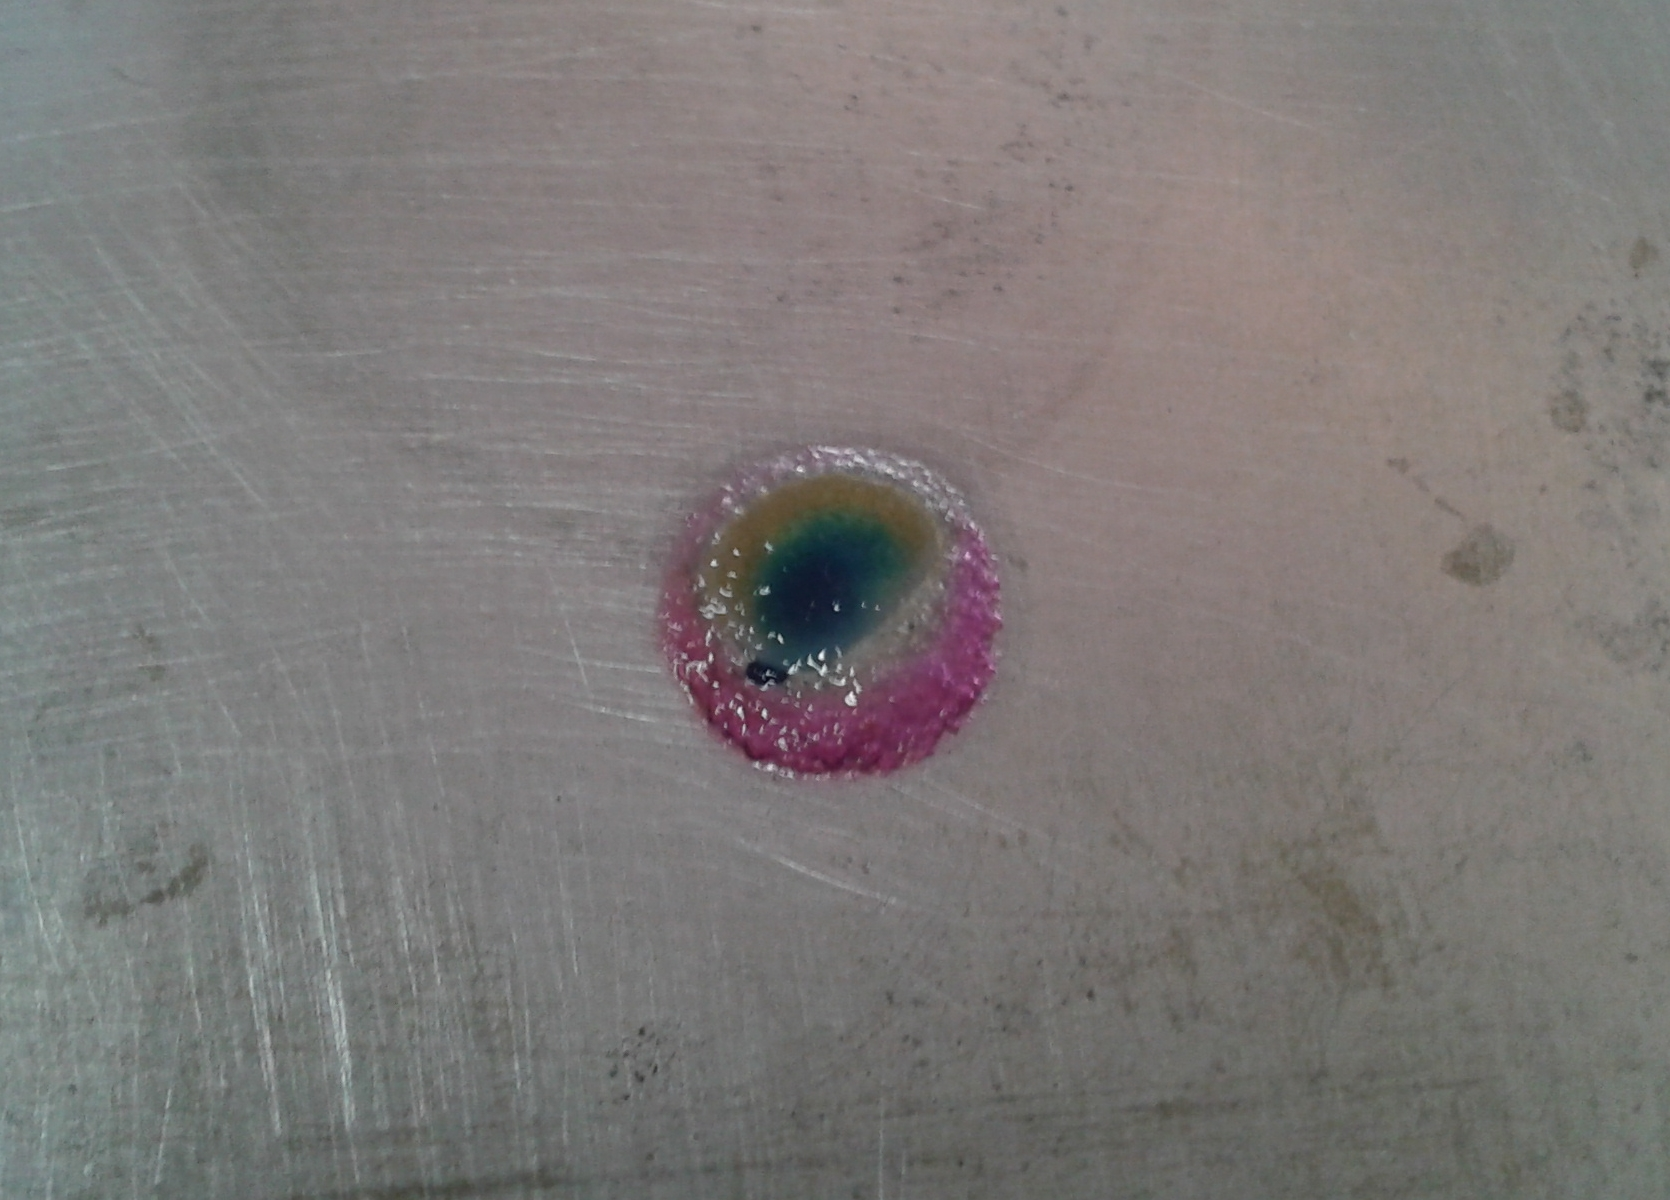
\includegraphics[scale=.13]{Chimie_Corrosion_Goutte.jpg}

\bsc{Fig. 1} : Goutte d'une solution de NaCl + $\epsilon$ $\varphi\varphi$ + $\epsilon$ K$^{+}$,\chemfig{Fe{(}CN{)}_6^{3-}} 	
\end{center}

\begin{itemize}		
\item Description : Une goutte de solution aqueuse de \chemfig{NaCl} contenant des traces de ph�nolphtal��ne et de complexes hexacianoferrique(III) est d�pos�e sur une plaque de Fer. 
\item Observations : A la p�riph�rie de la goutte, la solution devient rose : production d'ion \chemfig{HO^{-}} et au centre, la solution devient bleue : production de complexe \chemfig{Fe_3{(}Fe{(}CN{)}_{6}{)}_2} donc apparition d'ions \chemfig{Fe^{2+}} 
\item Interpr�tation : \begin{itemize}
\item A la p�riph�rie on a la r�action :  \schemestart \chemfig{O_2} \chemsign{+} 2\chemfig{H_2O} +4\chemfig{e^{-}} \arrow 4\chemfig{HO^{-}} \schemestop
\item Au centre, on a apparition de \chemfig{Fe^{2+}} : \schemestart \chemfig{Fe_{(s)}}  \arrow \chemfig{Fe^{2+}} \chemsign{+} 2\chemfig{e^{-}} \schemestop
\end{itemize}
\end{itemize}
\definecolor{zzqqww}{rgb}{0.6,0,0.4}
\definecolor{qqqqff}{rgb}{0,0,1}
\definecolor{ffqqqq}{rgb}{1,0,0}
\begin{center}
\begin{tikzpicture}[line cap=round,line join=round,>=triangle 45,x=1.0cm,y=1.0cm]
\clip(-7.95,-1.92) rectangle (7.89,2.78);
\draw [shift={(-1.27,-3.86)}] plot[domain=1.69:2.46,variable=\t]({1*6.1*cos(\t r)+0*6.1*sin(\t r)},{0*6.1*cos(\t r)+1*6.1*sin(\t r)});
\draw [shift={(0,-9.95)}] plot[domain=1.41:1.73,variable=\t]({1*12.32*cos(\t r)+0*12.32*sin(\t r)},{0*12.32*cos(\t r)+1*12.32*sin(\t r)});
\draw [shift={(1.27,-3.86)}] plot[domain=0.68:1.45,variable=\t]({1*6.1*cos(\t r)+0*6.1*sin(\t r)},{0*6.1*cos(\t r)+1*6.1*sin(\t r)});
\draw (-8,0)-- (8,0);
\draw (-7.5,1.54) node[anchor=north west] {$Air$};
\draw (-7.51,-0.44) node[anchor=north west] {$Fer$};
\draw(-3,0) circle (1cm);
\draw(3,0) circle (1cm);
\draw (-0.82,-0.29) node[anchor=north west] {$ Fe $};
\draw (0.22,-0.32) node[anchor=north west] {$Fe $};
\draw (-3.27,0.03) node[anchor=north west] {$ e^- $};
\draw (2.76,0.06) node[anchor=north west] {$ e^- $};
\draw [color=ffqqqq](-1.79,-0.46) node[anchor=north west] {$ e^- $};
\draw [color=ffqqqq](1.29,-0.41) node[anchor=north west] {$ e^- $};
\draw [->,color=ffqqqq] (-1.02,-0.62) -- (-2.14,-0.52);
\draw [->,color=ffqqqq] (1,-0.57) -- (2.11,-0.47);
\draw [color=qqqqff](0.27,1) node[anchor=north west] {$Fe^{2+} $};
\draw [color=qqqqff](-1.03,1) node[anchor=north west] {$Fe^{2+} $};
\draw [->] (-0.53,-0.26) -- (-0.52,0.28);
\draw [->] (0.52,-0.26) -- (0.54,0.28);
\draw (-3.8,0.62) node[anchor=north west] {$ O_2 $};
\draw (2.19,0.64) node[anchor=north west] {$ O_2 $};
\draw (-3.17,0.75) node[anchor=north west] {$ H_2O $};
\draw (2.83,0.79) node[anchor=north west] {$ H_2O $};
\draw [color=zzqqww](-5.34,0.72) node[anchor=north west] {$ HO^-$};
\draw [color=zzqqww](4.49,0.7) node[anchor=north west] {$ HO^-$};
\draw (-2.52,2.16) node[anchor=north west] {$Na^+,Cl^-$};
\draw (0.92,2.18) node[anchor=north west] {$Cl^-, Na^+$};
\draw [->] (-0.7,1.72) -- (-0.23,1.23);
\draw [->] (0.54,1.73) -- (0.19,1.23);
\draw [->] (-2.82,1.78) -- (-3.77,1.28);
\draw [->] (2.83,1.78) -- (3.79,1.2);
\draw [shift={(-3.99,0.14)},color=zzqqww]  plot[domain=0.69:2.18,variable=\t]({1*0.84*cos(\t r)+0*0.84*sin(\t r)},{0*0.84*cos(\t r)+1*0.84*sin(\t r)});
\draw [shift={(3.98,0.2)},color=zzqqww]  plot[domain=0.89:2.44,variable=\t]({1*0.87*cos(\t r)+0*0.87*sin(\t r)},{0*0.87*cos(\t r)+1*0.87*sin(\t r)});
\draw [->,color=zzqqww] (-4.47,0.82) -- (-4.72,0.66);
\draw [->,color=zzqqww] (4.52,0.88) -- (4.76,0.67);
\end{tikzpicture}
\end{center}
\noindent La force motrice de cette r�action est le gradient de concentration de dioxyg�ne dans l'eau : elle est plus importante � la p�riph�rie qu'au centre donc la concentration � la p�riph�rie doit diminuer par consommation d'\chemfig{O_2}.

\vspace{1cm}
\noindent \underline{G�n�ralisation :} toute cause d'h�t�rog�n�it� est source de corrosion diff�rentielle = soudures, d�fauts, un gradient de temp�rature...


\begin{center}
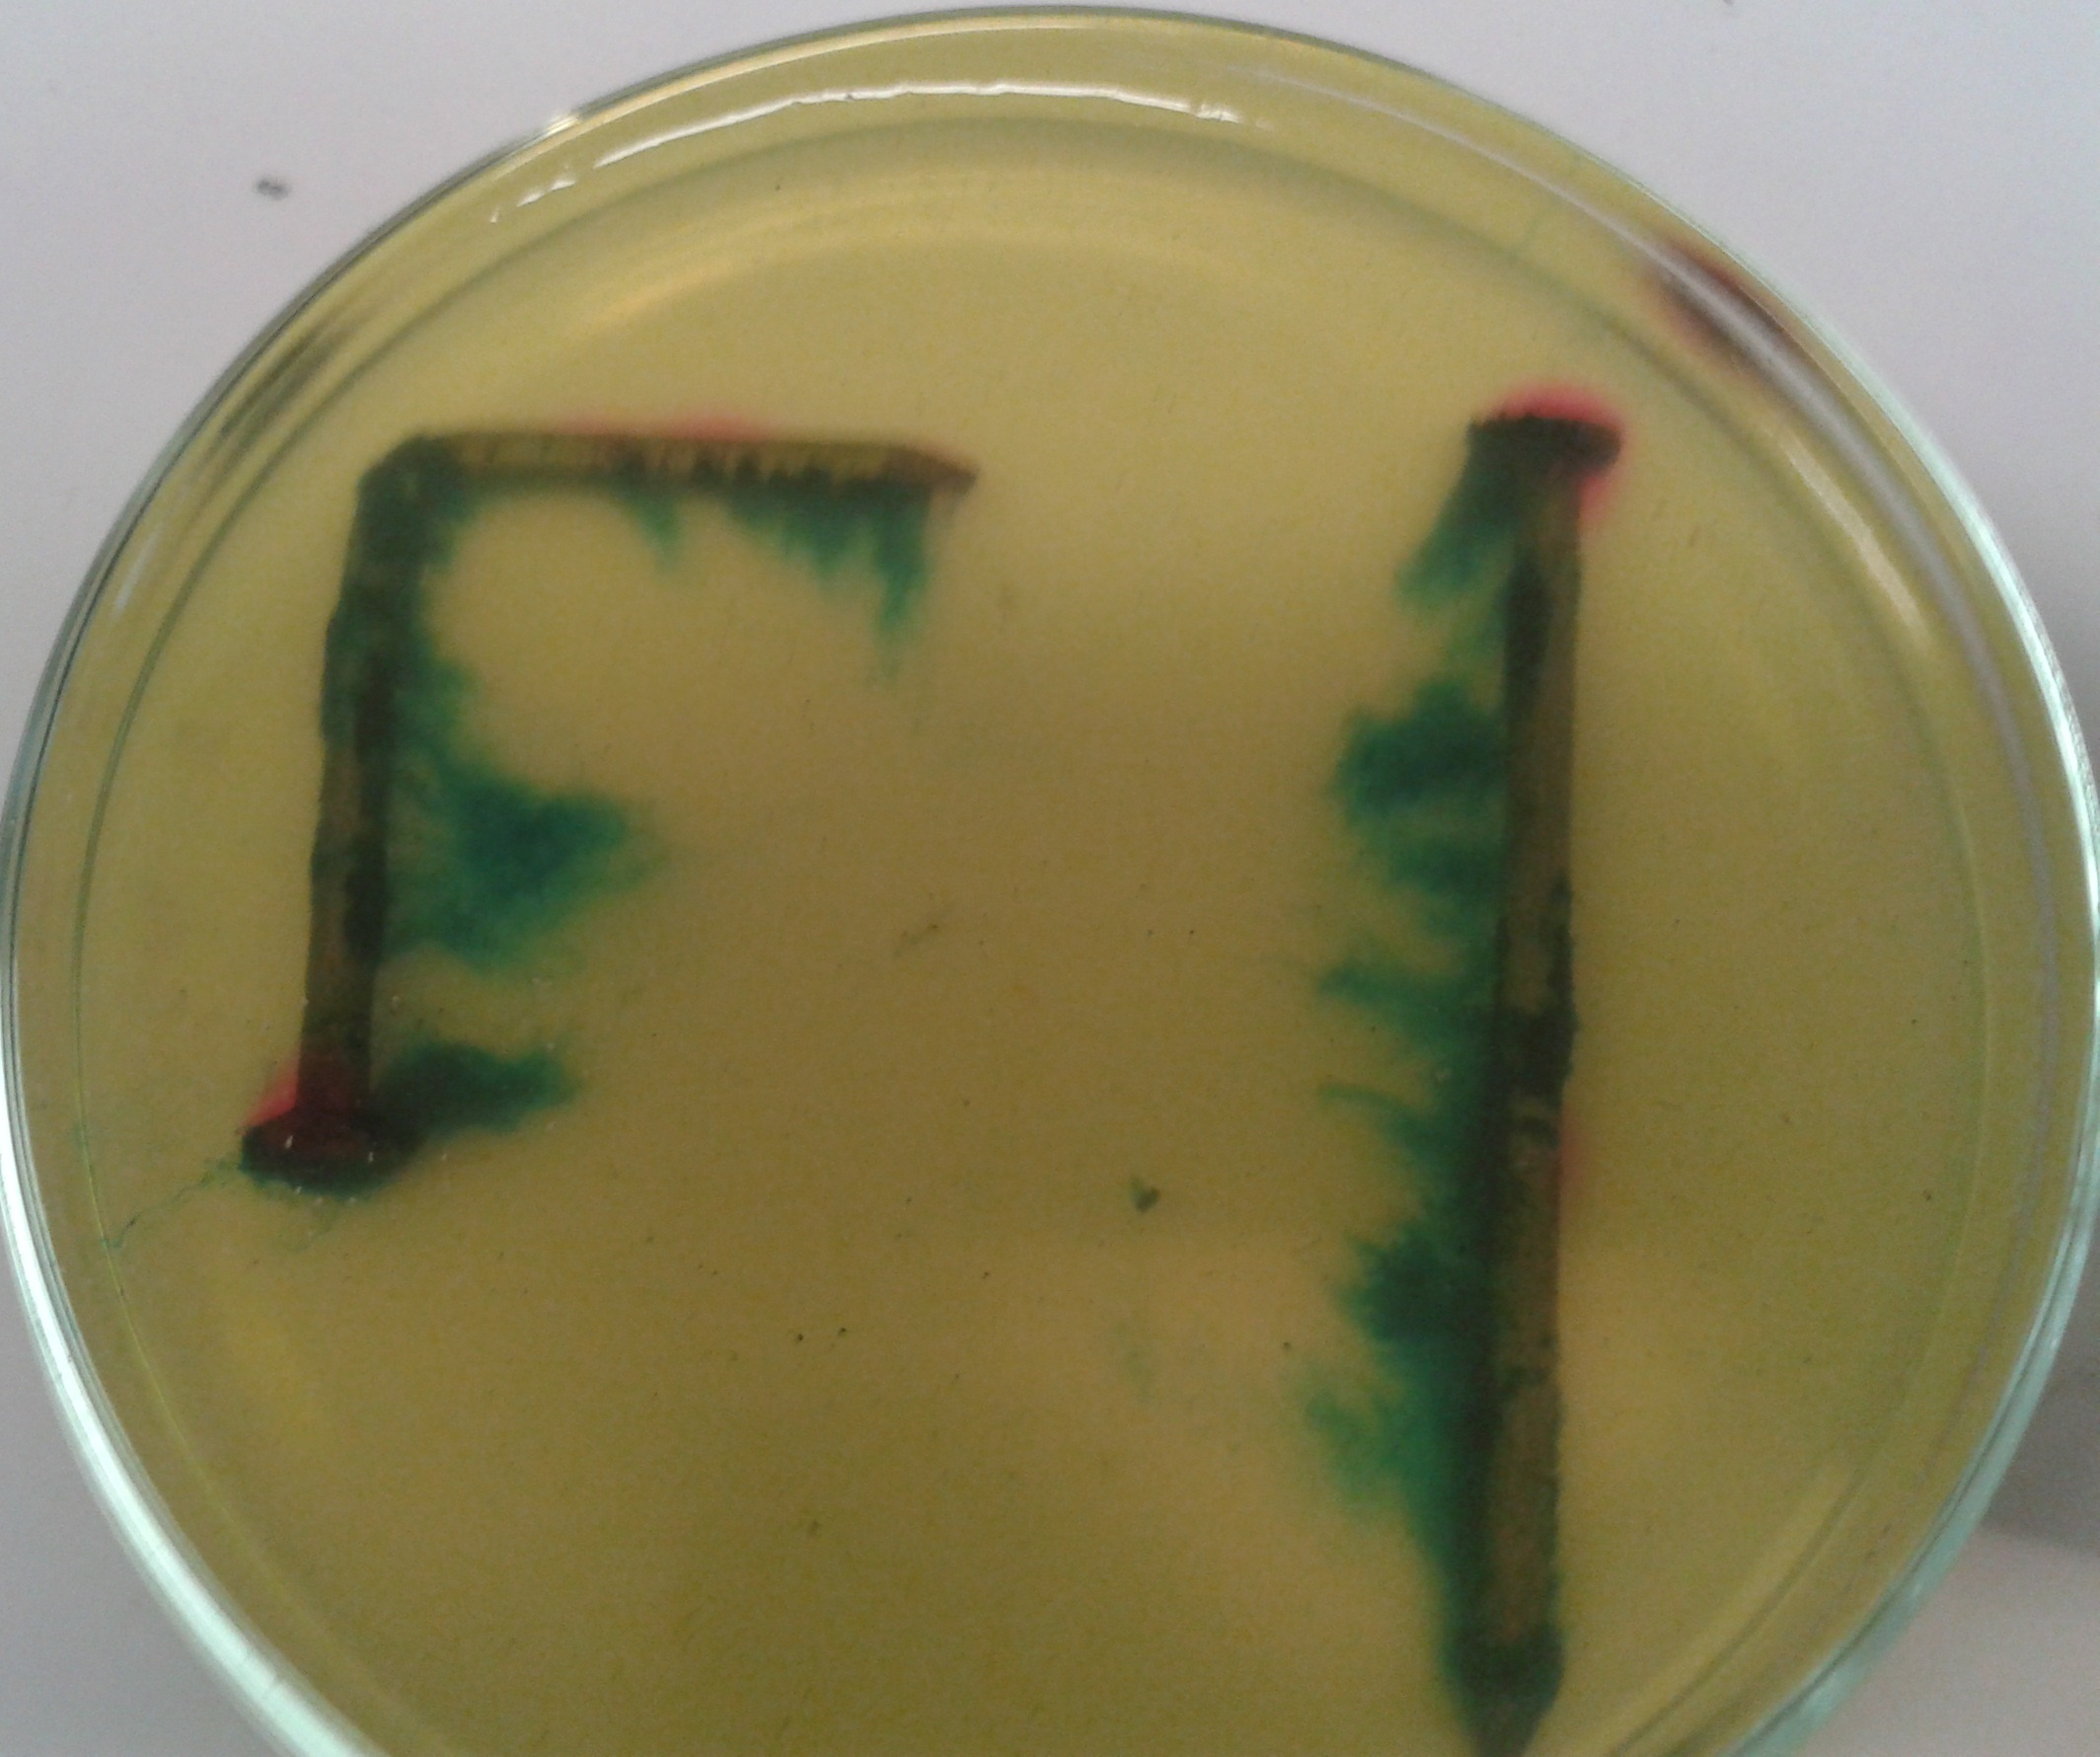
\includegraphics[scale=.1]{Chimie_Corrosion_Clou.jpg}

\bsc{Fig. 2} : Le fer s'oxyde (\chemfig{Fe_3{(}Fe{(}CN{)}_{6}{)}_2} bleu). 
\end{center}

	\section{Etude cin�tique}
		\subsection{couple $M^{2+}$/$M_{s}$}
		Une lame de cuivre plong�e dans une solution aqueuse de sulfate de cuivre subit une corrosion uniforme : on a un �quilibre dynamique entre les ions cuivres et le cuivre solide. Une �tude du diagramme i-E nous donne le potentiel d'�quilibre et le courant d'�change $i_0$. 
		\subsection{Couple $M^{2+}$/$M_{s}$ en pr�sence d'eau}
			Une lame de fer est plong�e dans une solution acide de sulfate de fer. Elle subit une corrosion diff�rentielle : en effet l'�tude du diagramme i-E montre que le courant de corrosion (repr�sentatif de la cin�tique de la r�action de Fe avec \chemfig{H^{+}}) est plus grand en valeur absolue que le courant d'�change $\Rightarrow$ sous contr�le cin�tique, c'est bien la corrosion diff�rentielle qui se produit.
	\section{M�thode de protection contre la corrosion}
			\subsection{Courbe de polarisation d'un m�tal}
				Certains m�taux donnent effectivement lieu au ph�nom�ne de passivation Ti, Cr... Pour l'acier (alliage Fe/C avec le \%C $\simeq$ 0,15-0,85), le carbone ne sert qu'� am�liorer les propri�t�s m�caniques du fer et n'a aucun effet sur la corrosion. 
				\\ Les m�taux passivables pr�sentent sur leurs courbes i-E des zones o� i=0 pour un large domaine de potentiel (appel� Potentiel de Flade) situ� entre l'oxydation du m�tal proprement dite et la transpassivation (disparition de la couche passivante). On voit alors que l'oxydation est auto-inhib�e. Pour le Fer, dans l'air humide, cette passivation ne s'observe pas. On cherche donc � rendre le Fer \og inoxydable \fg. Pour cela, on r�alise un alliage dont le le domaine de passivation est important dans l'air humide ou dans des conditions sp�cifiques. La plupart des aciers inoxydables contiennent du Chrome � plus de 12\% en masse. 
				\\ Pour certains m�taux (par exemple le titane) la couche naturellement form�e assure une passivation efficace. Pour d'autres (par exemple l'aluminium) la couche naturelle est peu efficace (\chemfig{Al_2O_3} est peu adh�rent). Dans de tels cas, on oxyde de fa�on contr�l�e ces m�taux de fa�on � avoir une formation lente d'une couche efficace (on parle par exemple d'aluminium anodis�)
			\subsection{Protection cathodique}
			\begin{itemize}
\item Principe : on am�ne la structure � prot�ger dans son domaine d'immunit� et l'y maintient. Dans ces conditions, le Fer est la cathode et son oxydation devient n�gligeable. 
\item Protection par courant impos� : la pi�ce � prot�ger est reli�e au p�le - d'un g�n�rateur de courant. Cette m�thode est surtout utilis�e pour les pi�ces enterr�es ou immerg�es. L'anode est constitu�e d'un bloc de graphite qu'il faut changer r�guli�rement.
\item Protection par anode sacrificielle : on court-circuite le fer avec un m�tal plus corrodable (par exemple le zinc, l'aluminium ou le mangan�se). Plus corrodable signifie que son courant de corrosion pour le potentiel d'�quilibre du Fer est plus grand que le courant d'�change du fer : la r�action d'oxydation du zinc solide est beaucoup plus rapide que celle du Fer, c'est donc lui qui disparait (c'est pourquoi on parle d'anode sacrificielle puisqu'on perd le m�tal)
\item Protection par un rev�tement m�tallique : \begin{itemize}
\item Par un m�tal plus corrodable que le fer : on recouvre la pi�ce de Fer � prot�ger par une couche de Zinc. Si on a rupture de la couche de zinc, le Fer est � nu mais on a une protection cathodique : le Zinc s'oxyde en \chemfig{Zn{(}OH{)}_2} qui est passivant donc autoinhibe la corrosion. 

\vspace{.5cm}
\begin{center}
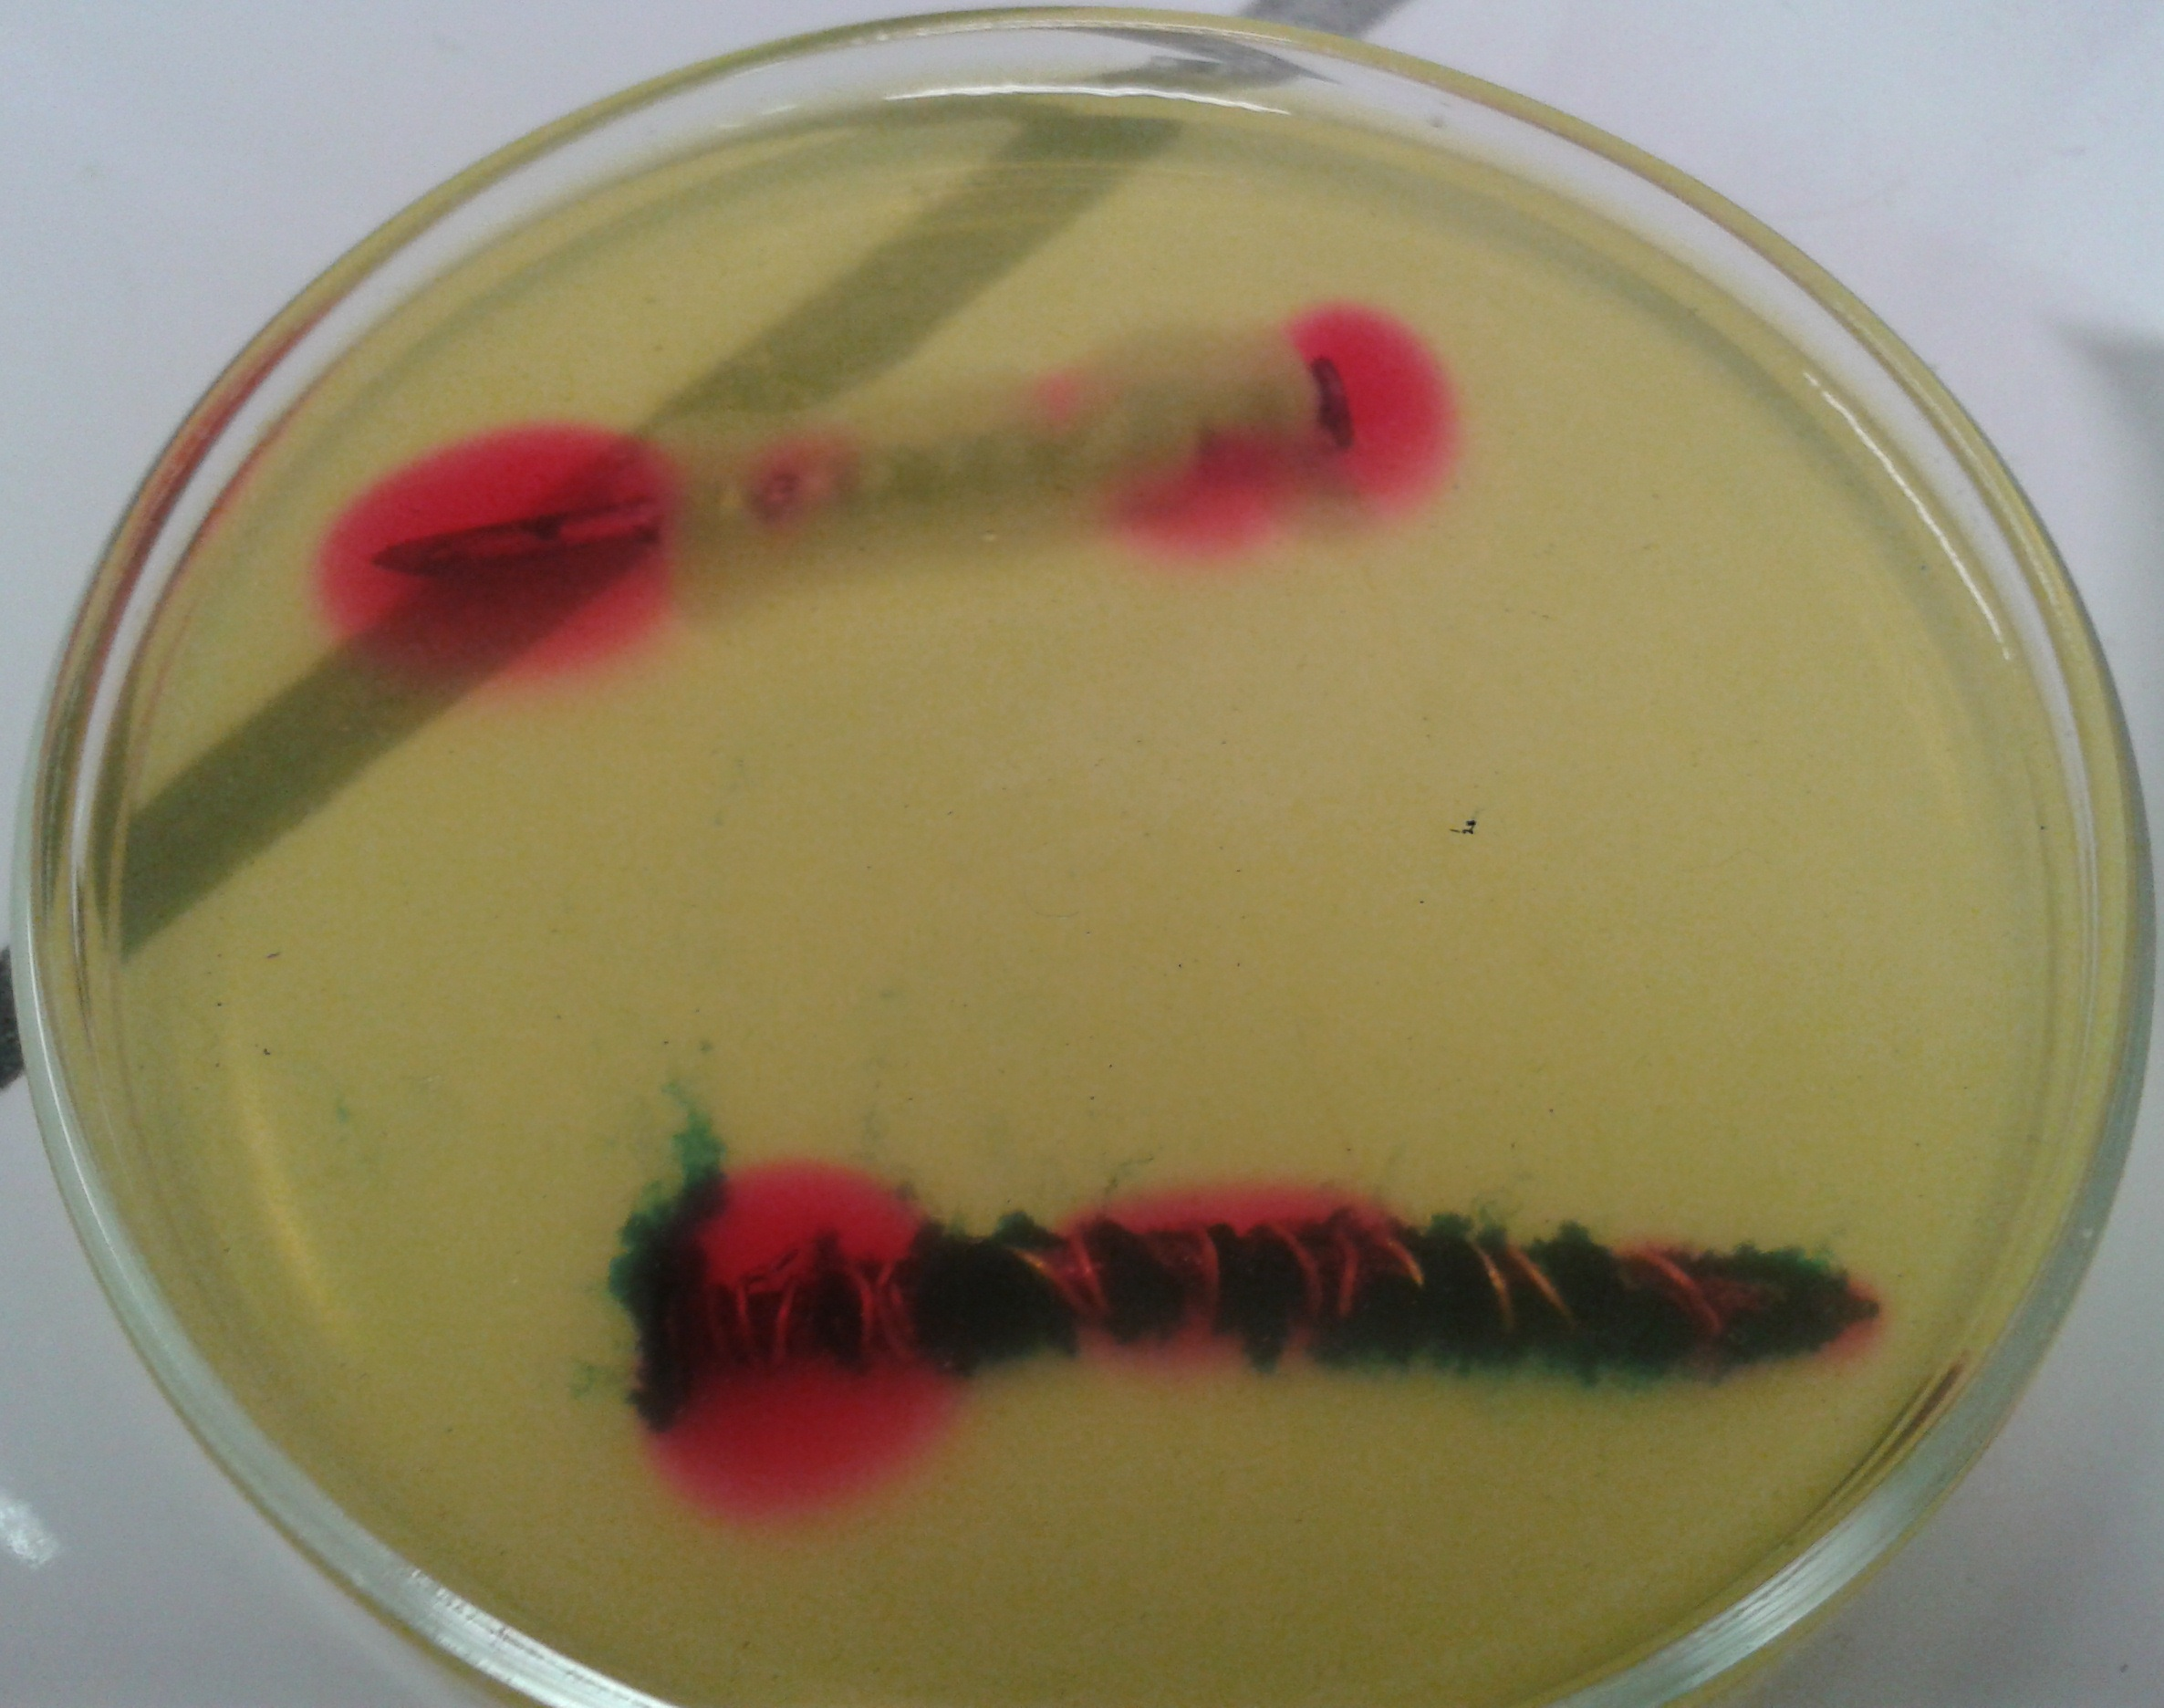
\includegraphics[scale=.1]{Chimie_Corrosion_Sacrificielle.jpg} 

\bsc{Fig. 3} \\ (Clou du haut) Un morceau de zinc est enroul� autour du clou, le zinc s'oxyde (\chemfig{Zn{(}OH{)}_2} blanc). \\ (Clou du bas) Un fil de cuivre est enroul� autour du clou, le fer s'oxyde (\chemfig{Fe_3{(}Fe{(}CN{)}_{6}{)}_2} bleu).
\end{center}

\vspace{.5cm}
\item Pour d�poser la couche de zinc protectrice, on plonge la pi�ce en fer, pr�alablement d�cap�e, d�graiss�e et pr�chauff�e dans un bain de Zinc$_{l}$ ou alors on utilise la m�thode d'�lectrozingage : la cathode est la pi�ce � zinguer, l'anode du Zn tr�s pur et l'�lectrolyte du \chemfig{Zn{(}OH{)}_{4}^{2-}} ou \chemfig{Zn{(}Cl{)}_{4}^{2-}}. On d�pose alors une couche d'environ 10 $\mu m$ de Zinc. 
\item Par un m�tal moins corrodable que le fer : par exemple une couche de Nickel. Si on a rupture de la couche protectrice de Ni, le Fer est � nu. Comme le Fer est plus corrodable que le Nickel, c'est lui qui est corrod� principalement. Cette protection est donc un facteur aggravant la corrosion.
\end{itemize}
\end{itemize}
\section{Conclusion}
	Il existe d'autre m�thodes : \begin{itemize}
\item la peinture
\item le rev�tement plastique
\item la transformation chimique superficielle
\end{itemize}
La corrosion a une importance �conomique colossale : chaque seconde, 2000 kg de Fer sont corrod�s et 20\% de l'acier produit dans le monde sert � remplacer les pi�ces corrod�es.

\end{document}

